% Audited English report. Build from this directory with latexmk -lualatex main-en.tex.
\documentclass[11pt,a4paper]{article}
\usepackage[english]{babel}
\usepackage{fontspec}
\setmainfont{Libertinus Serif}
\setsansfont{Libertinus Sans}
\setmonofont{Noto Sans Mono}[Scale=0.78]
\usepackage[margin=25mm]{geometry}
\usepackage{microtype,amsmath,amssymb,graphicx,booktabs,tabularx,longtable,array}
\usepackage{xcolor,tikz,fvextra,enumitem}
\usetikzlibrary{arrows.meta,positioning,calc}
\usepackage[section]{placeins}
\usepackage{needspace}
\usepackage[hidelinks]{hyperref}
\usepackage{xurl,fancyhdr}
\usepackage[font=small,labelfont=bf]{caption}
\definecolor{accent}{HTML}{126B65}
\tikzset{auditbox/.style={draw=accent,rounded corners=2pt,fill=accent!5,align=center,font=\small,text width=3cm,minimum height=10mm},auditarr/.style={-{Stealth},thick,draw=accent},auditlabel/.style={font=\scriptsize,fill=white,inner sep=2pt,align=center}}
\pagestyle{fancy}\fancyhf{}
\fancyhead[L]{\small VN-Edu LOD}\fancyhead[R]{\small English project report}
\fancyfoot[C]{\thepage}
\setlength{\headheight}{14pt}
\setlength{\parskip}{5pt}
\setlength{\emergencystretch}{3em}
\widowpenalty=10000
\clubpenalty=10000
\setlist{itemsep=3pt,topsep=4pt}
\newcommand{\term}[1]{\texttt{#1}}
\newcolumntype{P}[1]{>{\raggedright\arraybackslash}p{#1}}
\DefineVerbatimEnvironment{code}{Verbatim}{fontsize=\small,breaklines=true,breakanywhere=true,frame=single,rulecolor=\color{black!20}}
\BeforeBeginEnvironment{code}{\Needspace{12\baselineskip}}
% Generated by audit/release_metrics.py
\newcommand{\metricInstitutions}{297}
\newcommand{\metricHEIs}{268}
\newcommand{\metricPeople}{1{,}703}
\newcommand{\metricLeaders}{221}
\newcommand{\metricAlumni}{0}
\newcommand{\metricEducationParticipants}{1{,}482}
\newcommand{\metricObservations}{4{,}165}
\newcommand{\metricPrograms}{78}
\newcommand{\metricMajors}{37}
\newcommand{\metricCurrentProvinces}{34}
\newcommand{\metricFormerProvinces}{29}
\newcommand{\metricAssertedTriples}{59{,}392}
\newcommand{\metricInferredTriples}{23{,}014}
\newcommand{\metricLinkTriples}{3{,}557}
\newcommand{\metricOsmCoordinateTriples}{126}
\newcommand{\metricOntologyTriples}{948}
\newcommand{\metricUnionTriples}{87{,}162}
\newcommand{\metricMetadataTriples}{129}
\newcommand{\metricLocalResources}{6{,}413}
\newcommand{\metricClasses}{44}
\newcommand{\metricObjectProperties}{40}
\newcommand{\metricDataProperties}{29}
\newcommand{\metricFoundingConflicts}{5}
\newcommand{\metricWarnings}{33}
\newcommand{\metricViolations}{0}
\newcommand{\metricInformationResults}{1}

\hypersetup{pdftitle={VN-Edu LOD: Design, Implementation, and Critical Evaluation},pdfauthor={VN-Edu LOD project}}
\begin{document}
\hypersetup{pageanchor=false}
\begin{titlepage}
\centering
\vspace*{18mm}
{\sffamily\large SEMANTIC WEB PROJECT\par}
\vspace{18mm}
{\sffamily\bfseries\Huge VN-Edu LOD\par}
\vspace{8mm}
{\LARGE A Knowledge Graph of Vietnamese\par Higher-Education Institutions\par}
\vspace{10mm}
{\Large Design, Implementation, and Evidence-based Evaluation\par}
\vspace{10mm}
{\color{accent}\rule{0.65\textwidth}{1pt}\par}
\vspace{10mm}
{\large Revised English project report\par}
{\large Ontology 2.2 and integration edition: 8 October 2026\par}
\vfill
\begin{minipage}{0.9\textwidth}\small
This report presents the design and implementation of a Linked Open Data knowledge graph
for Vietnamese higher-education institutions. It combines a domain ontology, a reproducible
multi-source transformation pipeline, RDF publication, reasoning, validation, and SPARQL
access. The report is based on the corrected repository release and reports measured results
with their scope, rather than treating a successful query or a visualization as proof of
real-world truth.

Project repository:\\
\url{https://github.com/pham-ng/Vietnam-University-Knowledge-Graph-ver2}
\end{minipage}
\end{titlepage}
\hypersetup{pageanchor=true}

\begin{abstract}
VN-Edu LOD is an RDF knowledge graph for Vietnamese educational institutions. The project
integrates structured Wikidata records, Vietnamese Wikipedia material, and curated reference
tables into a common model of organizations, people, academic programs, and administrative
geography. The corrected snapshot contains \metricInstitutions{} educational organizations,
\metricPeople{} people, \metricCurrentProvinces{} current and \metricFormerProvinces{}
former province-level units, and \metricPrograms{} illustrative programs. Its central
technical contribution is a staged Bronze--Silver--Gold pipeline: source snapshots are
normalized into records, records are mapped to persistent HTTP IRIs, RDF is linked and
materialized, and the resulting union is released only after structural and semantic checks.

The ontology contains \metricClasses{} local classes, \metricObjectProperties{} object
properties, and \metricDataProperties{} datatype properties. OWL 2 RL profile checking,
rule-based materialization, SHACL validation, Apache Jena Fuseki/TDB2 acceptance tests,
and regression tests provide complementary evidence. The validated serving union contains
\metricUnionTriples{} distinct triples. The report separates ontology conformance,
reference-link agreement, data completeness, factual accuracy, and production readiness:
they are related engineering goals, but none is a substitute for the others. The result is
a reproducible educational Linked Data artifact with an explicit list of remaining evidence
requirements for authoritative, high-load deployment.
\end{abstract}
\noindent\textbf{Keywords:} knowledge graph; RDF; ontology; SHACL; SPARQL; entity resolution;
data provenance; Vietnamese higher education.
\clearpage\tableofcontents\clearpage
\listoffigures\clearpage
\listoftables\clearpage

\section{Project overview}
\subsection{Motivation and problem statement}
Information about a university is distributed across knowledge bases, encyclopedic articles,
institutional pages, and administrative reference data. The same institution may have several
names, identifiers, locations, or organizational relationships. These differences matter in
practice: a member school is not necessarily a branch campus, direct governance is not the
same as state oversight, and a former province is not interchangeable with its successor.
An RDF knowledge graph is useful here because it represents those distinctions as typed,
linkable statements that can be queried across sources.

VN-Edu LOD is an engineering case study of this integration problem. It is designed to
demonstrate a complete Semantic Web workflow, from source collection and URI assignment to
ontology-based transformation, reasoning, validation, publication, and query execution.
It is not presented as a complete official register of Vietnamese higher education. Names,
classifications, dates, and relationships describe the collected snapshot and the project's
documented extraction policies.

\subsection{Objectives and contributions}
The project has four practical objectives:
\begin{enumerate}
\item build a domain ontology that distinguishes organization, governance, people, education,
geography, identity, and temporal evidence;
\item transform heterogeneous records into persistent RDF resources and publish machine-readable
representations using Linked Data principles;
\item evaluate the release with OWL 2 RL profile checking, materialization, SHACL, SPARQL,
and automated regression tests; and
\item demonstrate reproducible execution with Apache Jena Fuseki and a controlled Silk
candidate-linking experiment.
\end{enumerate}

The resulting contributions are summarized in Table~\ref{tab:contributions}. This framing
follows a project-report structure: each contribution is paired with an artifact and an
evidence source, so that the report can distinguish implementation from evaluation.
\begin{table}[htbp]\centering\small
\caption{Project contributions and evidence.}\label{tab:contributions}
\begin{tabularx}{\textwidth}{p{3.0cm}XX}\toprule
Contribution & Implemented artifact & Evidence reported in this document \\\midrule
Domain model & OWL/Turtle ontology 2.2 with classes, properties, signatures, alignments, and selected chains & Protégé inspection, OWL 2 RL profile gate, ontology figures, and reasoning examples \\
Data integration & Bronze--Silver--Gold transformation pipeline, URI registry, provenance and conflict logs & Reproducible pipeline, mapping example, release fingerprints, and coverage counts \\
Linked publication & HTML, Turtle, JSON-LD, stable resource IRIs, link graph, and metadata & Publication checks, five-star assessment, and explicit licensing/identity scope \\
Operational checks & Flask read-only query path, Fuseki/TDB2 loader, CI workflows, SHACL and regression suite & End-to-end acceptance tables, security probes, and test results \\
\bottomrule
\end{tabularx}
\end{table}

\subsection{Research and evaluation questions}
The evaluation is organized around four questions:
\begin{enumerate}
\item Does the model distinguish the relationships needed for institutional, educational,
geographic, and governance queries without producing detected local contradictions?
\item Can the transformation reproduce a validated release while preserving resource identity
when labels or input order change?
\item What do the measurements establish about structure, coverage, link agreement, and
factual correctness, and which claims remain unsupported?
\item Can publication and query handling fail safely on stale releases, invalid input,
unapproved federation, and bounded overload?
\end{enumerate}

The review covers the source code, ontology, SHACL shapes, cached inputs, generated RDF,
tests, CI workflows, and earlier project documentation. Security counterexamples are
executed locally; external production endpoints are not used as attack targets.

\section{Semantic Web foundations and requirements}
\subsection{Standards used by the project}
RDF describes resources through triples. Subjects may be IRIs or blank nodes; predicates
are IRIs, and objects may additionally be literals. A graph is a set, so duplicate triples
do not increase its size. This matters when combining asserted data, ontology statements,
links, and inferred statements: their file counts cannot simply be added to obtain the
size of the union~\cite{rdf}.

OWL axioms express implications about the modeled world. A property's domain is not an
input-validation rule: using the property can entail that its subject belongs to that
domain. Similarly, a functional object property can imply equality between two values;
it does not necessarily reject the second value. The project therefore supplements
reasoning with explicit validation of asserted records. The OWL 2 profile specification
defines restrictions under which particular reasoning guarantees apply~\cite{owl}.

SHACL validates a supplied data graph against declared constraints~\cite{shacl}.
Conformance is relative to those constraints, not a claim that every statement is true.
Here, missing values for some descriptive fields generate warnings, while invalid
datatypes, selected cardinality violations, and hard constraints prevent publication.

SPARQL supplies query syntax and algebra for RDF, including optional patterns, aggregates,
and remote \term{SERVICE} clauses~\cite{sparql}. Exposing it over HTTP introduces an
execution boundary: query syntax, remote destinations, elapsed work, and publication state
must all be controlled independently of the user interface.

The project reuses identifiers and vocabulary from Wikidata, DBpedia, schema.org, FOAF,
SKOS, and PROV-O. PROV-O supports descriptions of derivation~\cite{prov}; whether the
provenance is attached to an entity, a graph, or an individual assertion determines what
can actually be traced. HTTP identifiers and useful representations support Linked Data
publication, while persistence requires more than generating readable slugs~\cite{uris}.

The standards are assigned different responsibilities. RDF and HTTP IRIs provide the data
model and Web identity; OWL provides class and property semantics; SHACL provides explicit
validation constraints; SPARQL provides query access; and Fuseki provides a storage/query
runtime. Silk is used only for an experimental candidate-linking task. This separation is
important because a tool boundary is not a semantic guarantee: loading RDF into Fuseki does
not mint IRIs, SHACL does not prove facts, and OWL profile membership does not certify data
accuracy.

\begin{table}[htbp]\centering\small
\caption{Design requirements and the mechanism used to address them.}\label{tab:requirements}
\begin{tabularx}{\textwidth}{p{3.2cm}XX}\toprule
Requirement & Design response & Verification boundary \\\midrule
Interoperability & RDF 1.1, OWL, SKOS, PROV-O, JSON-LD, HTTP IRIs & Syntax and profile checks; external vocabulary semantics are not fully imported \\
Identity stability & Canonical resource namespace and committed URI registry & URI-regression tests; migration is still required when source keys change \\
Semantic precision & Separate properties for governance, oversight, membership, branch, ownership, and geography & Domain/range inspection and competency queries \\
Data quality & JSON Schema, raw asserted checks, OWL 2 RL materialization, and SHACL & Release gate; warnings remain visible and are not silently converted to facts \\
Reproducibility & Cached inputs, fingerprints, pinned runtime versions, CI workflows, and machine-readable reports & Local reconstruction plus Linux and Windows Fuseki/Silk evidence \\
\bottomrule
\end{tabularx}
\end{table}

\section{Data sources and collection}
\subsection{Source roles}
Wikidata contributes identifiers, labels, institutional attributes, organizational links,
and person-related records. Vietnamese Wikipedia contributes infobox fields, descriptions,
historical text, and links between articles. DBpedia supplies candidate identity links and
some fallback values. Selected reference tables describe province mergers, regional
groupings, fields of study, majors, and example programs. Geocoding is used as a fallback
for location resolution and is not equivalent to an authoritative campus register.

\begin{table}[htbp]\centering\small
\caption{Source roles and integration treatment.}\label{tab:sources}
\begin{tabularx}{\textwidth}{p{3.0cm}p{4.0cm}X}\toprule
Source or input & Information used & Treatment in the release \\\midrule
Wikidata & Identifiers, labels, types, links, and person/organization attributes & Primary identity evidence when a stable identifier is available; provenance is retained \\
Vietnamese Wikipedia & Infobox values, article descriptions, revisions, and page links & Structured extraction and revision-specific provenance; not treated as an official register \\
DBpedia and other linked datasets & Candidate external resources and identity links & Interlinking evidence; uncertain matches remain outside accepted identity assertions \\
Reference tables & Provinces, mergers, regions, fields, majors, and sample programs & Curated integration inputs; programs are illustrative rather than a complete catalogue \\
Geocoding fallback & Location resolution when structured identifiers are missing & Convenience support only; not evidence of legal campus status \\
\bottomrule
\end{tabularx}
\end{table}

Wikipedia and Wikidata are interconnected community resources. Agreement between them is
useful corroborating evidence, but they must not be described as statistically independent
sources. Imported statements can share an origin, and one resource may repeat an error
from another. A disagreement log exposes selected conflicts; it does not establish which
source is correct.

The collection strategy combines article-category traversal, infobox parsing, and
Wikidata queries. Results are retained in JSON snapshots. The repository also ships a
compressed HTTP cache. In the revised default pipeline, a cache miss raises an error
instead of silently contacting a changing remote source. A fresh collection is an explicit
operation. Dependency installation may still require Internet access; the offline claim
applies to cached data collection and reconstruction after dependencies are installed.

\subsection{Scope and selection effects}
The snapshot is a discovered set of educational organizations, not a census. Filtering
removes unrelated articles and some records lacking sufficient cross-source evidence.
That policy can exclude legitimate but poorly documented institutions. Institutions with
more detailed encyclopedia coverage are more likely to have richer records. The same bias
is particularly strong for people linked through education records.

The retained higher-education classification includes name-based heuristics. A title
beginning with a familiar institution type is evidence used by the implementation; it is
not a substitute for a current legal decision. Counts of higher-education institutions
must therefore be read as counts under the project's classification policy.

Academic programs are illustrative hand-entered data. They demonstrate program-to-major
queries but do not support claims about a university's complete or current admissions
offerings. Similarly, a Wikidata education relation establishes recorded attendance or
education, not necessarily completion of a degree. The existing \term{Alumnus} class must
be interpreted with that limitation.

\section{Architecture and data management}
The implementation follows a layered architecture. Raw source material is kept separate
from normalized records; RDF generation is separate from reasoning; and validated output is
separate from publication. This organization is similar to the Bronze--Silver--Gold pattern
used in other Linked Data projects, but the names describe project artifacts rather than a
universal standard. The flow in Figure~\ref{fig:release-flow} is the release-level view;
the detailed transformation diagram appears in Section~\ref{sec:transform}.
\begin{figure}[htbp]\centering
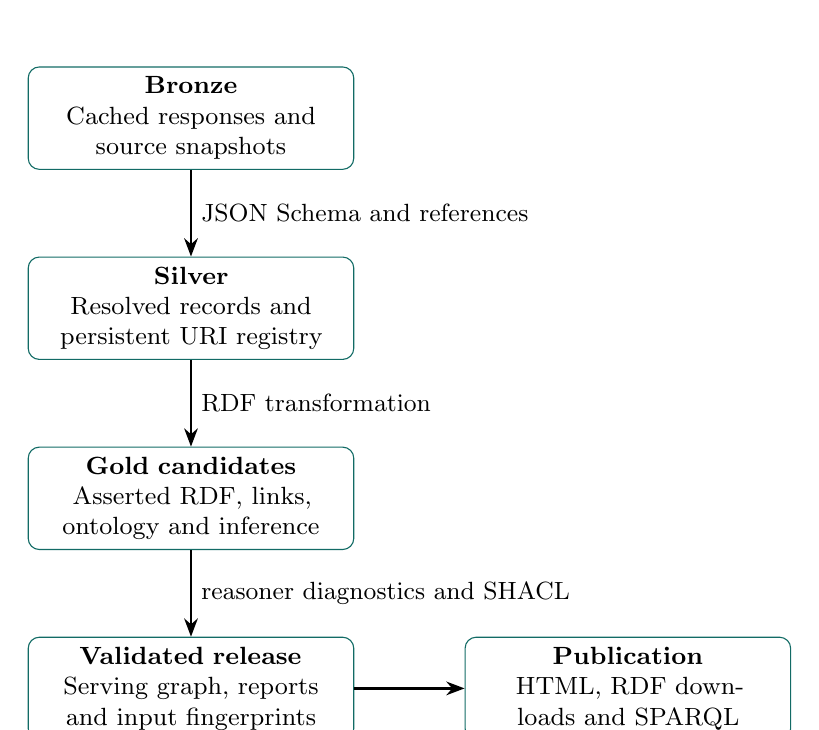
\begin{tikzpicture}[box/.style={draw=accent,rounded corners,align=center,text width=3.9cm,minimum height=1.3cm,font=\small},arr/.style={-{Stealth},thick},node distance=11mm]
\node[box] (bronze) {\textbf{Bronze}\\Cached responses and source snapshots};
\node[box,below=of bronze] (silver) {\textbf{Silver}\\Resolved records and persistent URI registry};
\node[box,below=of silver] (gold) {\textbf{Gold candidates}\\Asserted RDF, links, ontology and inference};
\node[box,below=of gold] (release) {\textbf{Validated release}\\Serving graph, reports and input fingerprints};
\node[box,right=14mm of release] (web) {\textbf{Publication}\\HTML, RDF downloads and SPARQL};
\draw[arr] (bronze)--node[right,font=\small]{JSON Schema and references}(silver);
\draw[arr] (silver)--node[right,font=\small]{RDF transformation}(gold);
\draw[arr] (gold)--node[right,font=\small]{reasoner diagnostics and SHACL}(release);
\draw[arr] (release)--(web);
\end{tikzpicture}
\caption[Validated release flow]{Release flow. A failed validation prevents replacement of validated inference and the serving graph; changed inputs invalidate the publication fingerprint.}
\label{fig:release-flow}
\end{figure}

\subsection{Layers and contracts}
Bronze stores responses and extraction snapshots. Silver contains institutions, people,
governing bodies, and provinces in a normalized JSON representation. Gold contains
asserted RDF, external links, selected instance-level entailments, and dataset metadata.
The layers improve inspectability, but the implementation rewrites snapshot files during
reconstruction. Bronze is therefore not an immutable append-only archive; Git revisions
provide versioned snapshots.

Silver validation checks schema constraints and selected cross-field rules. The audit
adds checks for future years, impossible calendar dates, missing cross-collection
references, and invalid leadership references. These checks complement, rather than
replace, semantic review of the extraction policy.

After RDF generation, literal ranges and functional-field cardinalities are validated
on the raw asserted graph, independently of equality in the closure. The rule engine's own error
messages are retained in the consistency diagnostics. SHACL then checks the asserted and
retained inferred graph. A failure stops the release step. On success, a validation record
binds the checked release to its ontology, shapes, Silver files, component RDF files, and
serving graph. The publisher rejects missing or stale validation records.

Fingerprints normalize text line endings to LF so that Git checkout on Windows and Linux
does not create false stale-release failures. This is a content-integrity check, not a
cryptographic signature or a guarantee against someone deliberately editing both the
inputs and validation record. Reproduction of RDF is evaluated semantically; timestamps,
blank-node labels, and serialization order can change without changing graph meaning.

\subsection{Identity and URI persistence}
A readable slug is used when a resource is first assigned a local URI. The revised minter
consults the committed \term{uri\_map.json} before allocating anything new. Renaming an
entity or inserting another entity with the same label does not change a registered URI.
Retired identifiers remain reserved. Source-key changes, such as a new QID replacing an
article-based key, still require an explicit identity migration policy.

The previous person integration merged unidentified leaders by normalized personal name
across all institutions. The audit found six names used across multiple institutions;
splitting these records adds seven person records. This does not prove that seven new
real people exist. It represents uncertainty conservatively: records without a shared
identifier are separated by institution until identity can be established. The former
ambiguous URI is reserved but is not asserted as identical to either replacement.

\subsection{Provenance and disputed values}
Institution records use \term{prov:wasDerivedFrom} to reference Wikidata items and
specific Wikipedia revisions. Conflict and fallback logs provide additional evidence for
some chosen fields. This is entity-level provenance plus partial field-level logging;
the project does not yet attach complete provenance to every triple. A Wikidata entity
URI is also not a pinned statement revision.

The earliest reported foundation year is the current integration policy and may refer to
a predecessor. Five records contain a different year in the infobox foundation date.
The revised exporter retains such a date under \term{vnedu:reportedFoundingDate}, rather
than asserting it as an unqualified \term{schema:foundingDate}. This preserves evidence
without pretending that the historical ambiguity has been adjudicated. Distinguishing
predecessor origin, legal establishment, and opening would require dated event records
and authoritative supporting sources.

\section{System and software architecture}
\label{sec:software-architecture}
The project is implemented as a batch-oriented Python application with separate data,
semantic, publication, and verification responsibilities. Figure~\ref{fig:system-architecture}
shows the complete system from external sources to user-facing artifacts. Figure~\ref{fig:software-architecture}
maps that flow to the repository's executable components. The diagrams are complementary:
the first explains the data life cycle, while the second explains the software boundaries.

\begin{figure}[htbp]\centering
\resizebox{\textwidth}{!}{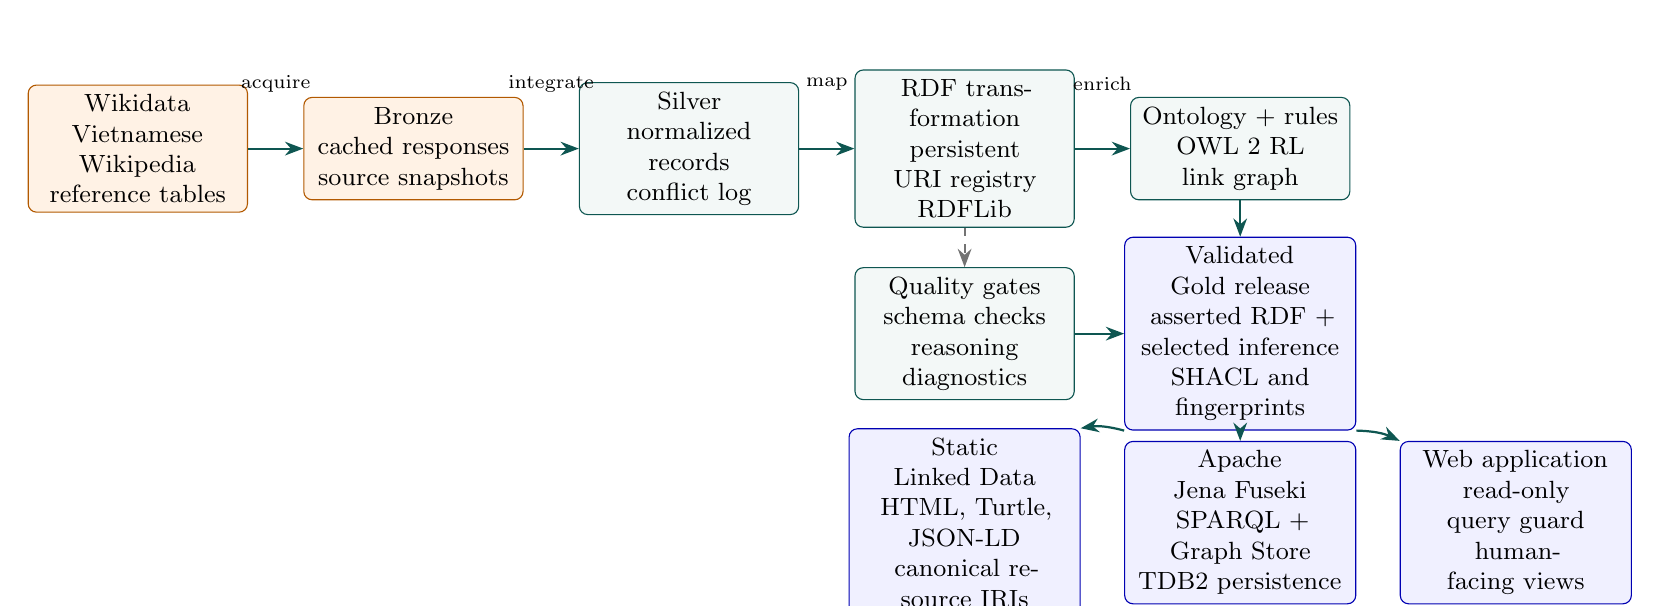
\begin{tikzpicture}[
  node distance=7mm and 8mm,
  layer/.style={draw=accent!80!black, rounded corners=3pt, fill=accent!5, align=center, font=\small, text width=2.55cm, minimum height=13mm},
  source/.style={draw=orange!70!black, rounded corners=3pt, fill=orange!10, align=center, font=\small, text width=2.55cm, minimum height=13mm},
  artifact/.style={draw=blue!70!black, rounded corners=3pt, fill=blue!6, align=center, font=\small, text width=2.7cm, minimum height=13mm},
  arrow/.style={-{Stealth}, thick, draw=accent!80!black},
  sidearrow/.style={-{Stealth}, dashed, thick, draw=black!55}
]
\node[source] (sources) at (0,0) {Wikidata\\Vietnamese Wikipedia\\reference tables};
\node[source] (bronze) at (3.5,0) {Bronze\\cached responses\\source snapshots};
\node[layer] (silver) at (7,0) {Silver\\normalized records\\conflict log};
\node[layer] (transform) at (10.5,0) {RDF transformation\\persistent URI registry\\RDFLib};
\node[layer] (semantic) at (14,0) {Ontology + rules\\OWL 2 RL\\link graph};

\node[layer] (quality) at (10.5,-2.35) {Quality gates\\schema checks\\reasoning diagnostics};
\node[artifact] (release) at (14,-2.35) {Validated Gold release\\asserted RDF + selected inference\\SHACL and fingerprints};
\node[artifact] (static) at (10.5,-4.75) {Static Linked Data\\HTML, Turtle, JSON-LD\\canonical resource IRIs};
\node[artifact] (fuseki) at (14,-4.75) {Apache Jena Fuseki\\SPARQL + Graph Store\\TDB2 persistence};
\node[artifact] (app) at (17.5,-4.75) {Web application\\read-only query guard\\human-facing views};

\draw[arrow] (sources)--(bronze);
\draw[arrow] (bronze)--(silver);
\draw[arrow] (silver)--(transform);
\draw[arrow] (transform)--(semantic);
\draw[arrow] (semantic)--(release);
\draw[arrow] (quality)--(release);
\draw[sidearrow] (transform)--(quality);
\draw[arrow] (release.south west) to[bend right=12] (static.north east);
\draw[arrow] (release)--(fuseki);
\draw[arrow] (release.south east) to[bend left=12] (app.north west);

\node[font=\scriptsize, align=center] at (1.75,0.82) {acquire};
\node[font=\scriptsize, align=center] at (5.25,0.82) {integrate};
\node[font=\scriptsize, align=center] at (8.75,0.82) {map};
\node[font=\scriptsize, align=center] at (12.25,0.82) {enrich};
\end{tikzpicture}
}
\caption[Overall VN-Edu LOD architecture]{Overall architecture of VN-Edu LOD. Source material is
collected and normalized before RDF generation; ontology enrichment and quality gates produce a
validated release that can be published statically, queried through the application, or loaded
into Apache Jena Fuseki.}
\label{fig:system-architecture}
\end{figure}

\begin{figure}[htbp]\centering
\resizebox{\textwidth}{!}{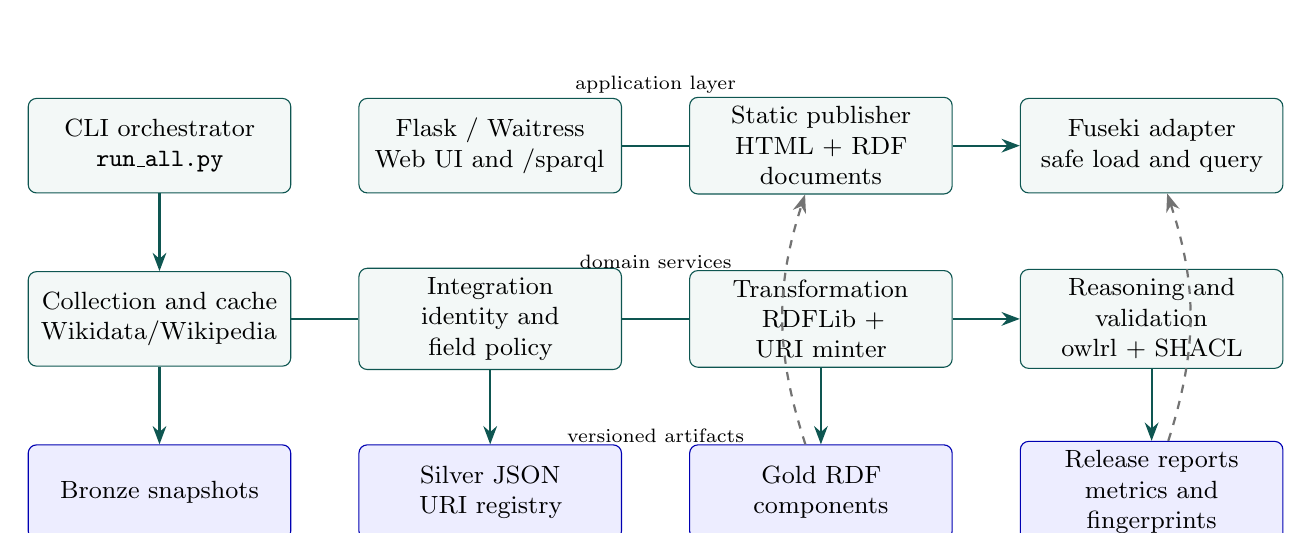
\begin{tikzpicture}[
  node distance=7mm and 8mm,
  box/.style={draw=accent!80!black, rounded corners=3pt, fill=accent!5, align=center, font=\small, text width=3.1cm, minimum height=12mm},
  data/.style={draw=blue!70!black, rounded corners=3pt, fill=blue!7, align=center, font=\small, text width=3.1cm, minimum height=12mm},
  edge/.style={-{Stealth}, thick, draw=accent!80!black},
  aux/.style={-{Stealth}, dashed, thick, draw=black!55}
]
\node[box] (cli) at (0,0) {CLI orchestrator\\\texttt{run\_all.py}};
\node[box] (web) at (4.2,0) {Flask / Waitress\\Web UI and /sparql};
\node[box] (rdfdocs) at (8.4,0) {Static publisher\\HTML + RDF documents};
\node[box] (fuseki) at (12.6,0) {Fuseki adapter\\safe load and query};

\node[box] (collect) at (0,-2.2) {Collection and cache\\Wikidata/Wikipedia};
\node[box] (integrate) at (4.2,-2.2) {Integration\\identity and field policy};
\node[box] (transform) at (8.4,-2.2) {Transformation\\RDFLib + URI minter};
\node[box] (reason) at (12.6,-2.2) {Reasoning and validation\\owlrl + SHACL};

\node[data] (raw) at (0,-4.4) {Bronze snapshots};
\node[data] (silver) at (4.2,-4.4) {Silver JSON\\URI registry};
\node[data] (rdf) at (8.4,-4.4) {Gold RDF components};
\node[data] (reports) at (12.6,-4.4) {Release reports\\metrics and fingerprints};

\draw[edge] (cli)--(collect);
\draw[edge] (collect)--(integrate)--(transform)--(reason);
\draw[edge] (web)--(rdfdocs)--(fuseki);
\draw[edge] (collect)--(raw);
\draw[edge] (integrate)--(silver);
\draw[edge] (transform)--(rdf);
\draw[edge] (reason)--(reports);
\draw[aux] (rdf) to[bend left=18] (rdfdocs);
\draw[aux] (reports) to[bend right=18] (fuseki);

\node[font=\scriptsize, align=center] at (6.3,0.78) {application layer};
\node[font=\scriptsize, align=center] at (6.3,-1.48) {domain services};
\node[font=\scriptsize, align=center] at (6.3,-3.68) {versioned artifacts};
\end{tikzpicture}
}
\caption[Software architecture and repository components]{Software architecture. The CLI orchestrator
coordinates domain services, while versioned artifacts connect the services to the static publisher,
web application, and Fuseki adapter. Dashed arrows indicate artifact hand-off rather than direct
runtime calls.}
\label{fig:software-architecture}
\end{figure}

\subsection{Component responsibilities}
The collection layer obtains structured records and cached source responses. The integration
layer applies identity, field-precedence, normalization, and conflict policies. The RDF
transformer assigns or reuses resource IRIs, emits typed literals and object links, and keeps
the asserted graph separate from inferred output. The semantic layer applies the local ontology,
selected OWL/RDF rules, external links, and qualified observations. The release layer runs
raw-data checks, OWL diagnostics, SHACL, metric generation, graph-isomorphism checks, and
fingerprint validation before a serving artifact is accepted.

The web application is a consumer of the release rather than the source of truth. Its local
RDFLib backend is useful for an isolated read-only view; the optional Fuseki adapter provides
the tested HTTP/TDB2 path. The static publisher produces resource pages and RDF downloads for
Linked Data clients. This separation makes it possible to test the transformation and semantic
artifacts without requiring a running web server.

\subsection{Technology choices}
Python and RDFLib were retained for transparent transformation and easy regression testing.
OWL API and Protégé are used to inspect the ontology and check its OWL 2 RL profile. GraphDB
is useful for interactive repository exploration and visualization, but its layout is not the
formal specification. Apache Jena Fuseki 6.2.0 is used as the RDF HTTP server and TDB2
persistence target in the end-to-end acceptance workflow. Silk Framework 3.6.0 is isolated
as a candidate-linking experiment so that uncertain matches cannot silently enter the release.

\begin{table}[htbp]\centering\small
\caption{Main software components and their boundaries.}\label{tab:software-components}
\begin{tabularx}{\textwidth}{p{3.2cm}p{4.2cm}X}\toprule
Component & Responsibility & Boundary \\\midrule
\texttt{run\_all.py} and pipeline scripts & Orchestrate collection, integration, transformation, reasoning and publication & Batch execution; not a long-running RDF server \\
RDFLib and Python validators & Create RDF, apply local policies, inspect graphs, and run regression checks & Does not replace formal OWL profile checking or production load testing \\
Protégé/OWL API & Inspect ontology axioms and profile membership & Does not decide whether source facts are true \\
Flask/Waitress application & Read-only UI and guarded SPARQL access & Uses bounded local execution; external TLS/proxy policy remains operational \\
Apache Jena Fuseki/TDB2 & Persistent RDF store and SPARQL/Graph Store protocol & Requires deployment hardening, authentication, backups, and measured capacity \\
\bottomrule
\end{tabularx}
\end{table}

\section{Data transformation and knowledge-graph population}
\label{sec:transform}
The transformation is implemented in Python. Apache Jena Fuseki is not the transformer: it
is the RDF store and query server used after the graph has been created. Figure~\ref{fig:transform-flow}
shows the implemented path from source records to the validated serving union.

\begin{figure}[htbp]\centering
\resizebox{\textwidth}{!}{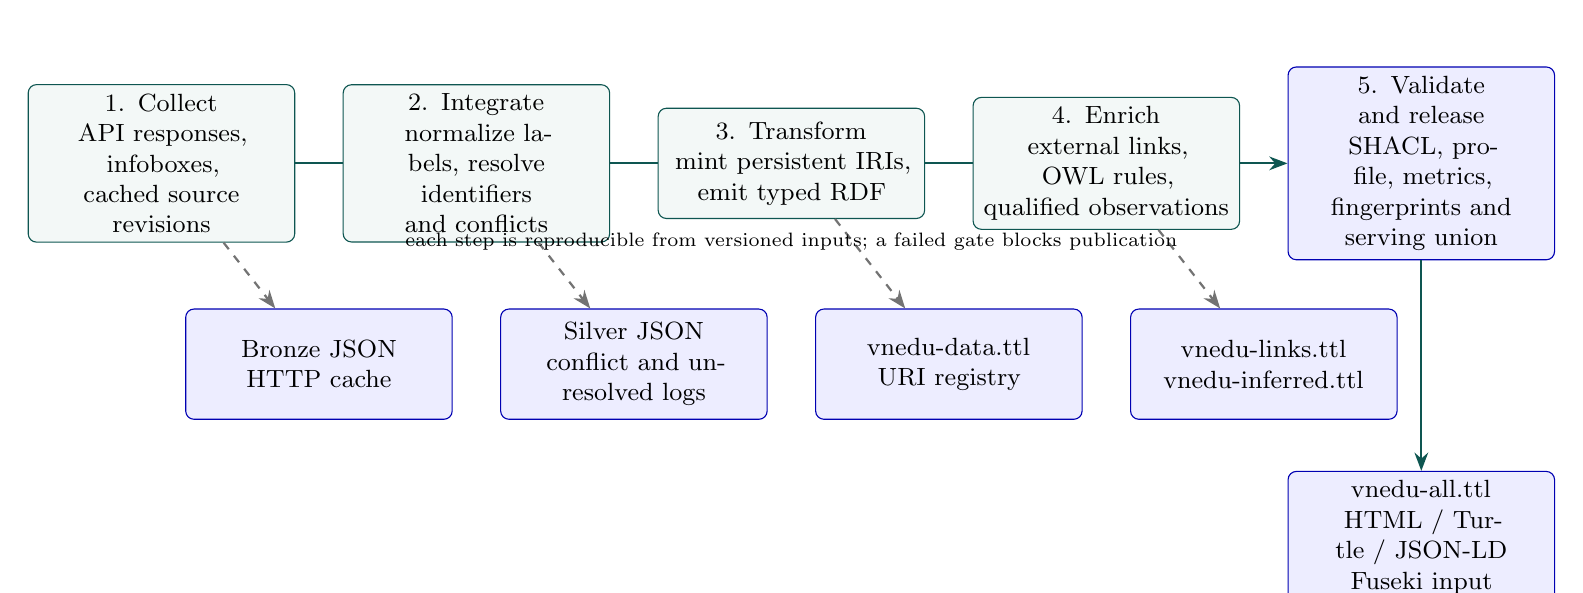
\begin{tikzpicture}[
  node distance=8mm and 7mm,
  tstep/.style={draw=accent!80!black, rounded corners=3pt, fill=accent!5, align=center, font=\small, text width=3.15cm, minimum height=14mm},
  toutput/.style={draw=blue!70!black, rounded corners=3pt, fill=blue!7, align=center, font=\small, text width=3.15cm, minimum height=14mm},
  arr/.style={-{Stealth}, thick, draw=accent!80!black},
  aux/.style={-{Stealth}, dashed, thick, draw=black!55}
]
\node[tstep] (s1) at (0,0) {1. Collect\\API responses, infoboxes,\\cached source revisions};
\node[tstep] (s2) at (4.0,0) {2. Integrate\\normalize labels, resolve\\identifiers and conflicts};
\node[tstep] (s3) at (8.0,0) {3. Transform\\mint persistent IRIs,\\emit typed RDF};
\node[tstep] (s4) at (12.0,0) {4. Enrich\\external links, OWL rules,\\qualified observations};
\node[toutput] (s5) at (16.0,0) {5. Validate and release\\SHACL, profile, metrics,\\fingerprints and serving union};

\node[toutput] (a1) at (2.0,-2.55) {Bronze JSON\\HTTP cache};
\node[toutput] (a2) at (6.0,-2.55) {Silver JSON\\conflict and unresolved logs};
\node[toutput] (a3) at (10.0,-2.55) {vnedu-data.ttl\\URI registry};
\node[toutput] (a4) at (14.0,-2.55) {vnedu-links.ttl\\vnedu-inferred.ttl};
\node[toutput] (a5) at (16.0,-4.75) {vnedu-all.ttl\\HTML / Turtle / JSON-LD\\Fuseki input};

\draw[arr] (s1)--(s2)--(s3)--(s4)--(s5);
\draw[aux] (s1)--(a1);
\draw[aux] (s2)--(a2);
\draw[aux] (s3)--(a3);
\draw[aux] (s4)--(a4);
\draw[arr] (s5)--(a5);
\node[font=\scriptsize, align=center] at (8,-1.0) {each step is reproducible from versioned inputs; a failed gate blocks publication};
\end{tikzpicture}
}
\caption[Data transformation workflow]{Data transformation workflow. Each stage produces a
reviewable artifact. The final serving union is emitted only after RDF, ontology, reasoning,
SHACL, metric, and fingerprint checks succeed.}
\label{fig:transform-flow}
\end{figure}

\subsection{Bronze layer: collection and source preservation}
The Bronze layer stores cached responses, structured snapshots, and source context. Wikidata
queries contribute identifiers and structured attributes; Vietnamese Wikipedia contributes
infobox fields, article text, links, and revision identifiers; reference tables contribute
administrative crosswalks, fields, majors, and illustrative programs. A cache miss fails by
default during reconstruction, so a normal build does not silently change its input by
contacting a live endpoint. Fresh collection is an explicit operation.

\subsection{Silver layer: integration and normalization}
The integration stage joins records through stable identifiers when available, normalizes
labels and values, resolves organization references, and records conflicts or unresolved
targets. It produces normalized JSON for institutions, people, governing bodies, provinces,
and programs. The Silver layer is where source policies are applied; it is not yet an OWL
graph. For example, a ministry associated with a private institution is represented as
reported state oversight rather than automatically asserted as direct ownership or governance.

\subsection{Gold layer: RDF transformation, linking and reasoning}
The RDF transformer maps each normalized record to a class and a set of properties in
\texttt{ontology/vnedu.ttl}. Persistent IRIs are reused from \texttt{uri\_map.json}; a readable
slug is only the initial allocation key. Literal values receive explicit language tags and
datatypes, while resource-valued fields become object IRIs. External links are written to a
separate link graph. The reasoner applies the local ontology and selected OWL/RDF rules, and
the release retains selected instance-level entailments rather than treating every internal
closure statement as an authoritative source fact.

\subsection{Concrete Silver-to-RDF mapping}
Table~\ref{tab:mapping} follows the shipped Silver record \texttt{Q3075696}, Hanoi University
of Science and Technology. It demonstrates the mapping rules; it is not an independent
verification of the institution's current legal status or leadership.

\begin{table}[htbp]\centering\small
\caption{Selected Silver-to-RDF mappings for one institution record.}\label{tab:mapping}
\begin{tabularx}{\textwidth}{p{3.3cm}Xp{4.4cm}}\toprule
Silver input & RDF output & Rule or qualification \\\midrule
\texttt{key = Q3075696} & Subject \texttt{u:dai-hoc-bach-khoa-ha-noi} & Reuse the persistent registry; a label change does not mint a new IRI. \\
\texttt{kind = University} & \texttt{rdf:type vnedu:University} & Classification follows the integration policy, not Fuseki. \\
\texttt{name\_vi} & \texttt{rdfs:label} and \texttt{skos:prefLabel} with \texttt{@vi} & Preserve language information. \\
\texttt{founding\_year = 1956} & \texttt{vnedu:foundingYear ``1956'' \textasciicircum\textasciicircum xsd:integer} & May refer to predecessor origin; the event meaning remains qualified. \\
\texttt{province = Q1858} & \texttt{vnedu:locatedIn} the registered Hanoi IRI & Use an object resource, not a province-name literal. \\
\texttt{ownership = public} & \texttt{vnedu:ownership vnedu:PublicOwnership} & Supports the public-institution classification rule. \\
\texttt{viwiki\_revid} & \texttt{prov:wasDerivedFrom} a Wikipedia oldid IRI & Entity-level source context, not complete assertion-level provenance. \\
\bottomrule
\end{tabularx}
\end{table}

Missing optional values normally produce no triple; they are not converted into empty strings,
zeros, or claims of non-existence. Reference programs are identified using the institution slug
and major code. This gives a stable demonstration resource, but it does not distinguish every
curriculum, degree level, delivery mode, or academic year without additional identifiers.

\subsection{Release boundary}
The serving graph is the set union of ontology, asserted data, selected inference, external
links, and metadata. Component files remain available for inspection, but loading the union
into a default graph does not recreate named-graph provenance. The workflow is therefore a
reproducible staged batch process, not a transaction covering every intermediate file. The
validated release record binds the accepted output to its inputs and rejects stale publication
or Fuseki loading attempts.


\section{Ontology design and relationship semantics}
\subsection{Design method}
The ontology was designed from competency questions rather than from the visual shape of
the source tables. Candidate concepts were grouped into modules, each relation was assigned
a domain and range only when the data semantics justified it, and stronger axioms were kept
separate from data-quality rules. The resulting model is therefore a TBox: it describes
classes, properties, signatures, hierarchies, alignments, and selected entailment patterns.
The institutional records, people, programs, and locations are the ABox. SHACL shapes and
raw-record checks validate the ABox without pretending that every optional field is complete.

This distinction also explains why the ontology diagram should not be read as a relational
database schema. A relational diagram emphasizes tables and cardinalities; an OWL diagram
emphasizes concepts, property semantics, and possible entailments under the open-world
assumption. The project uses an ER/UML-like projection for readability, while the Turtle
axioms, Protégé inspection, profile check, and reasoner output remain authoritative.

\subsection{Modules}
The ontology has \metricClasses{} named local classes, \metricObjectProperties{} local
object properties, and \metricDataProperties{} local datatype properties in the audited
release. Table~\ref{tab:modules} summarizes the main relationship choices.
Figures~\ref{fig:ontology-er-relation-map} and~\ref{fig:tbox-architecture} visualize the
implemented axioms, while Figure~\ref{fig:abox-instance-neighborhood} shows a populated
individual-level neighborhood. Classes, property signatures, and instances are distinguished
explicitly.
\begin{table}[htbp]\centering\small
\caption{Main modules and intended distinctions.}\label{tab:modules}
\begin{tabularx}{\textwidth}{p{2.6cm}XX}\toprule
Module & Main entities or properties & Interpretation \\\midrule
Organizations & Institution, governing body, company; memberOf, branchOf, governedBy, ownedBy & Membership, branch status, governance, and ownership are separate relations. \\
Oversight & stateManagedBy & General state oversight is distinct from direct governance. \\
People & Person, InstitutionLeader, Alumnus; rector, director, councilChair & Leadership roles differ; education records do not certify graduation. \\
Geography & Province, FormerProvince, Region; locatedIn, partOf, mergedInto & Geographic crosswalks support aggregation under successor boundaries. \\
Education & AcademicProgram, Major, FieldOfStudy; offersProgram, ofMajor, inField & Example programs connect institutions to subjects; these are not an official offering inventory. \\
Identity & owl:sameAs, skos:closeMatch, foaf:isPrimaryTopicOf & Identity, approximate concept mapping, and document-topic links are not interchangeable. \\
\bottomrule\end{tabularx}
\end{table}

Disjointness axioms separate selected organizational and geographic categories. Their
usefulness depends on defensible category definitions. A statement that violates a
disjointness axiom could indicate erroneous data or an overly rigid ontology, so a
detected conflict should trigger inspection rather than automatic deletion of evidence.

Vocabulary alignments use subclass and subproperty relationships. Such alignments still
carry logical implications; choosing a weaker alignment than equivalence does not make
it semantically harmless. The current inference run does not import and validate the
complete external ontologies. Its absence of detected conflicts therefore applies to the
local reasoning scope, not every possible external combination.

\subsection{Visual specification of ontology 2.2}
\begin{figure}[htbp]\centering
\IfFileExists{docs/report/figures/ontology-er-relation-map.png}{%
  \includegraphics[width=\textwidth,height=0.78\textheight,keepaspectratio]{docs/report/figures/ontology-er-relation-map.png}%
}{%
  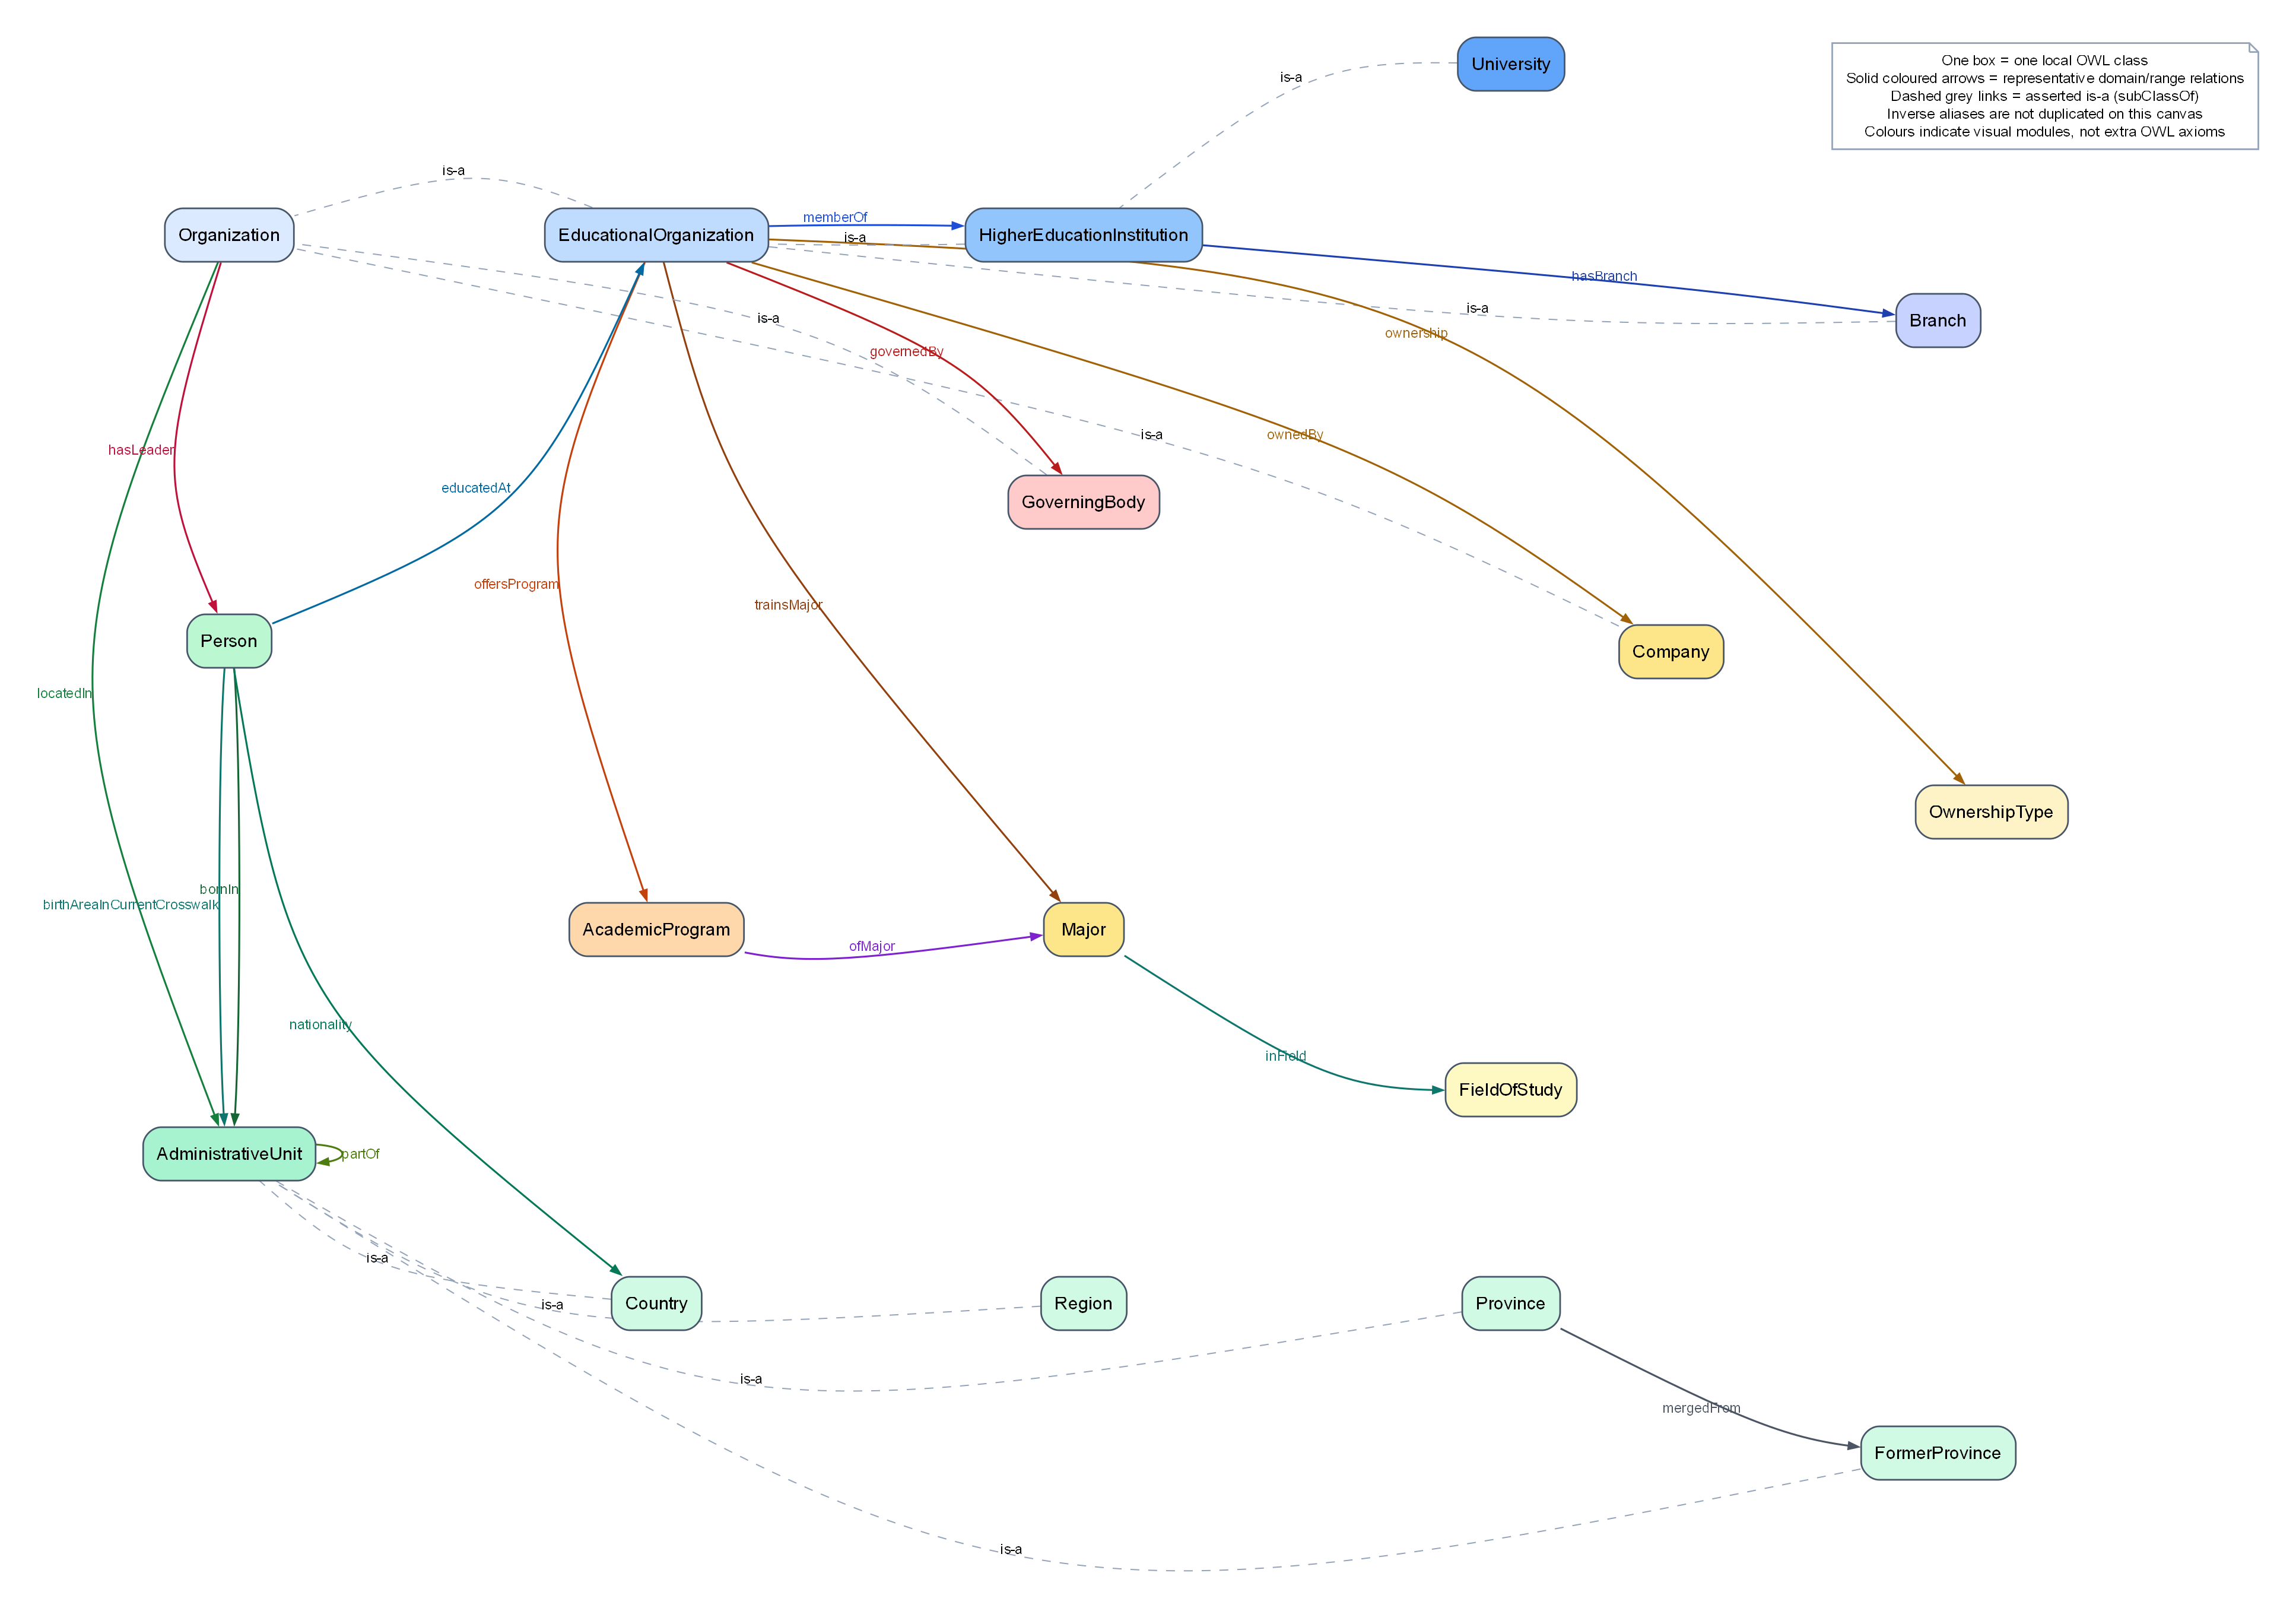
\includegraphics[width=\textwidth,height=0.78\textheight,keepaspectratio]{figures/ontology-er-relation-map.png}%
}
\caption[Main unique-node ontology map]{Main unique-node ontology map generated from the validated local OWL model. Each local class is rendered exactly once. Solid coloured arrows are asserted domain--range relations; dashed grey links are asserted \texttt{rdfs:subClassOf} axioms. The map uses one representative direction for inverse pairs so that it remains readable; the exact property inventory is documented separately. Coloured regions are presentation modules only and do not add OWL axioms.}\label{fig:ontology-er-relation-map}
\end{figure}

The map is the primary human-readable description of the ontology. It is intentionally closer to an ER/UML or GraphRAG schema than to a raw triple dump: organizations, people, education, governance, ownership and geography are shown as distinct conceptual modules, while every class remains a single node. Its layout is generated deterministically from the Turtle source, not drawn by hand or inferred from a screenshot. The source model is checked independently with the OWL API bundled with Protégé, OWL~2~RL materialization, SHACL validation and SPARQL regression queries. Therefore the figure is a readable projection of checked axioms, not a substitute for the formal validation artifacts.

\begin{figure}[htbp]\centering
\IfFileExists{docs/report/figures/ontology-protege-screenshot.png}{%
  \includegraphics[width=\textwidth]{docs/report/figures/ontology-protege-screenshot.png}%
}{%
  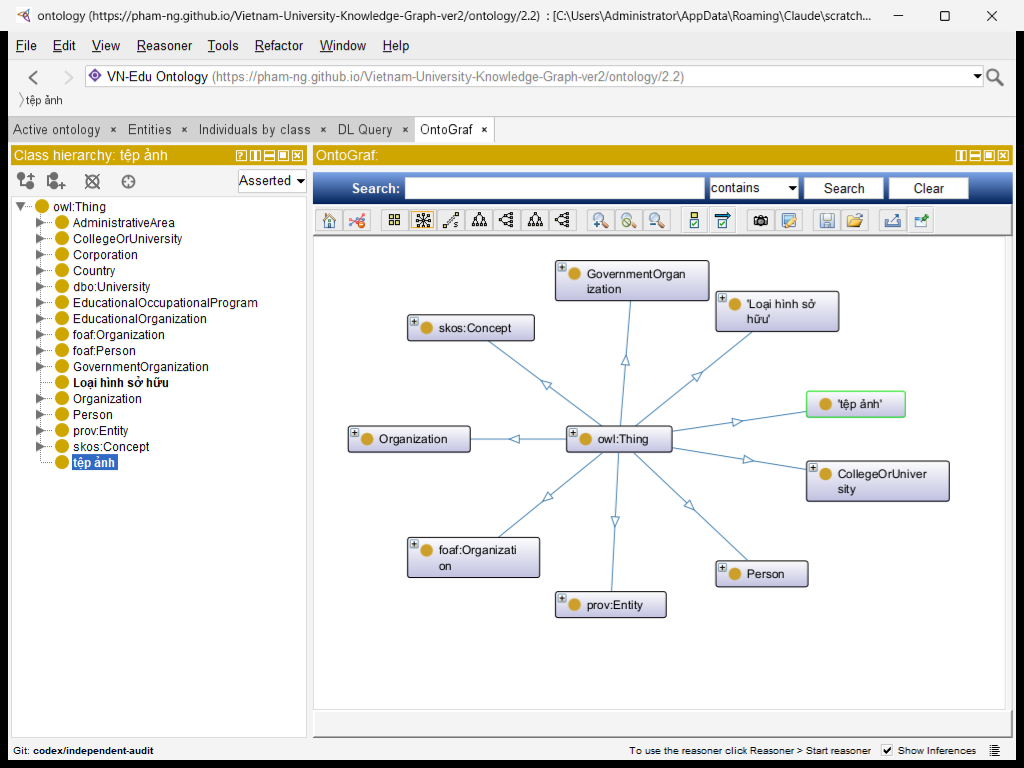
\includegraphics[width=\textwidth]{figures/ontology-protege-screenshot.png}%
}
\caption[Protégé OntoGraf view of ontology 2.2]{Direct screenshot of Protégé 5.6.7 with the OntoGraf plug-in,
after loading the committed \texttt{ontology/vnedu.ttl}. The class hierarchy is shown at left and the
selected ontology graph at right; the graph was laid out by OntoGraf and includes the selected
OWL classes and their asserted subclass relations.}
\label{fig:ontology-overview}
\end{figure}

\begin{figure}[htbp]\centering
\IfFileExists{docs/report/figures/ontology-protege-relations.png}{%
  \includegraphics[width=\textwidth]{docs/report/figures/ontology-protege-relations.png}%
}{%
  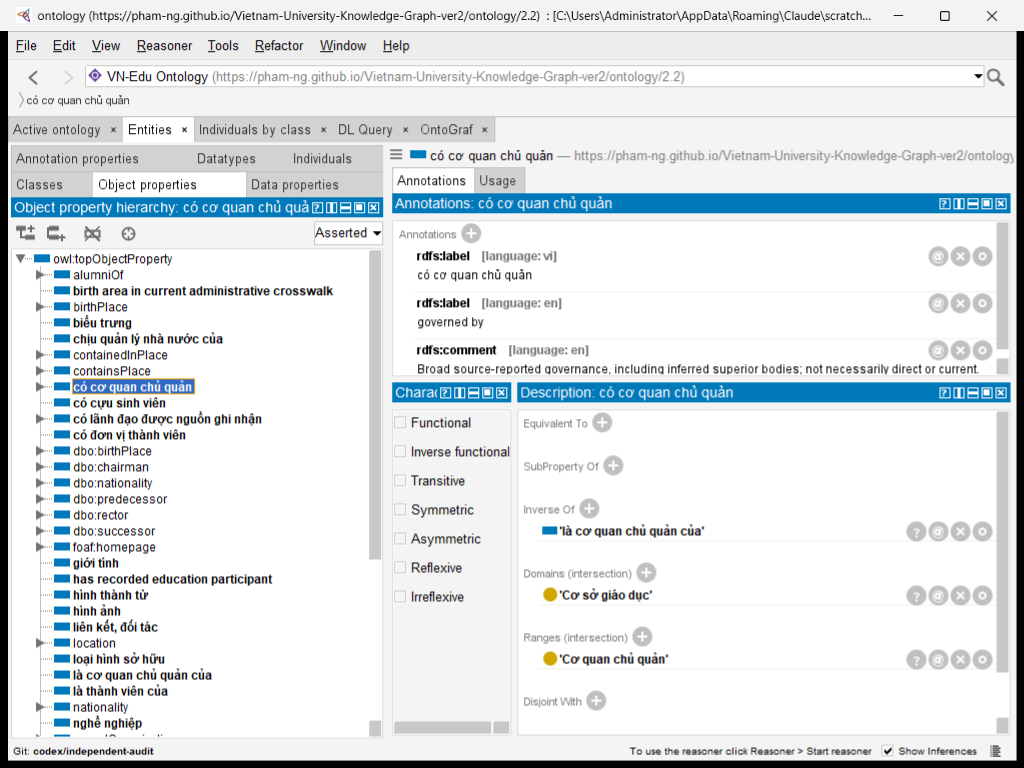
\includegraphics[width=\textwidth]{figures/ontology-protege-relations.png}%
}
\caption[Protégé object-property signature]{Direct screenshot of Protégé's Object properties view for
the committed ontology. The selected \term{governedBy} relation is displayed with bilingual labels,
its comment, domain \term{EducationalOrganization}, range \term{GoverningBody}, and its inverse
relation. This is the property-signature view used to verify that the graph has database-like
domain--relationship--range discipline; it is not a hand-drawn diagram.}\label{fig:ontology-protege-relations}
\end{figure}

Protégé is retained as the direct ontology-inspection tool for class and property axioms. GraphDB and Apache Jena Fuseki are retained as execution checks for repository loading, reasoning and SPARQL end-to-end behaviour; their screenshots are intentionally omitted from this section so that the main ontology explanation is not dominated by tool-specific layouts. This separation is important: a workbench layout is a user-interface projection, whereas the OWL axioms, reasoner output and query tests are the evidence for correctness.

\clearpage
\begin{figure}[htbp]\centering
\IfFileExists{docs/report/figures/ontology-tbox-hierarchy-clean.png}{%
  \includegraphics[width=\textwidth,height=0.84\textheight,keepaspectratio]{docs/report/figures/ontology-tbox-hierarchy-clean.png}%
}{%
  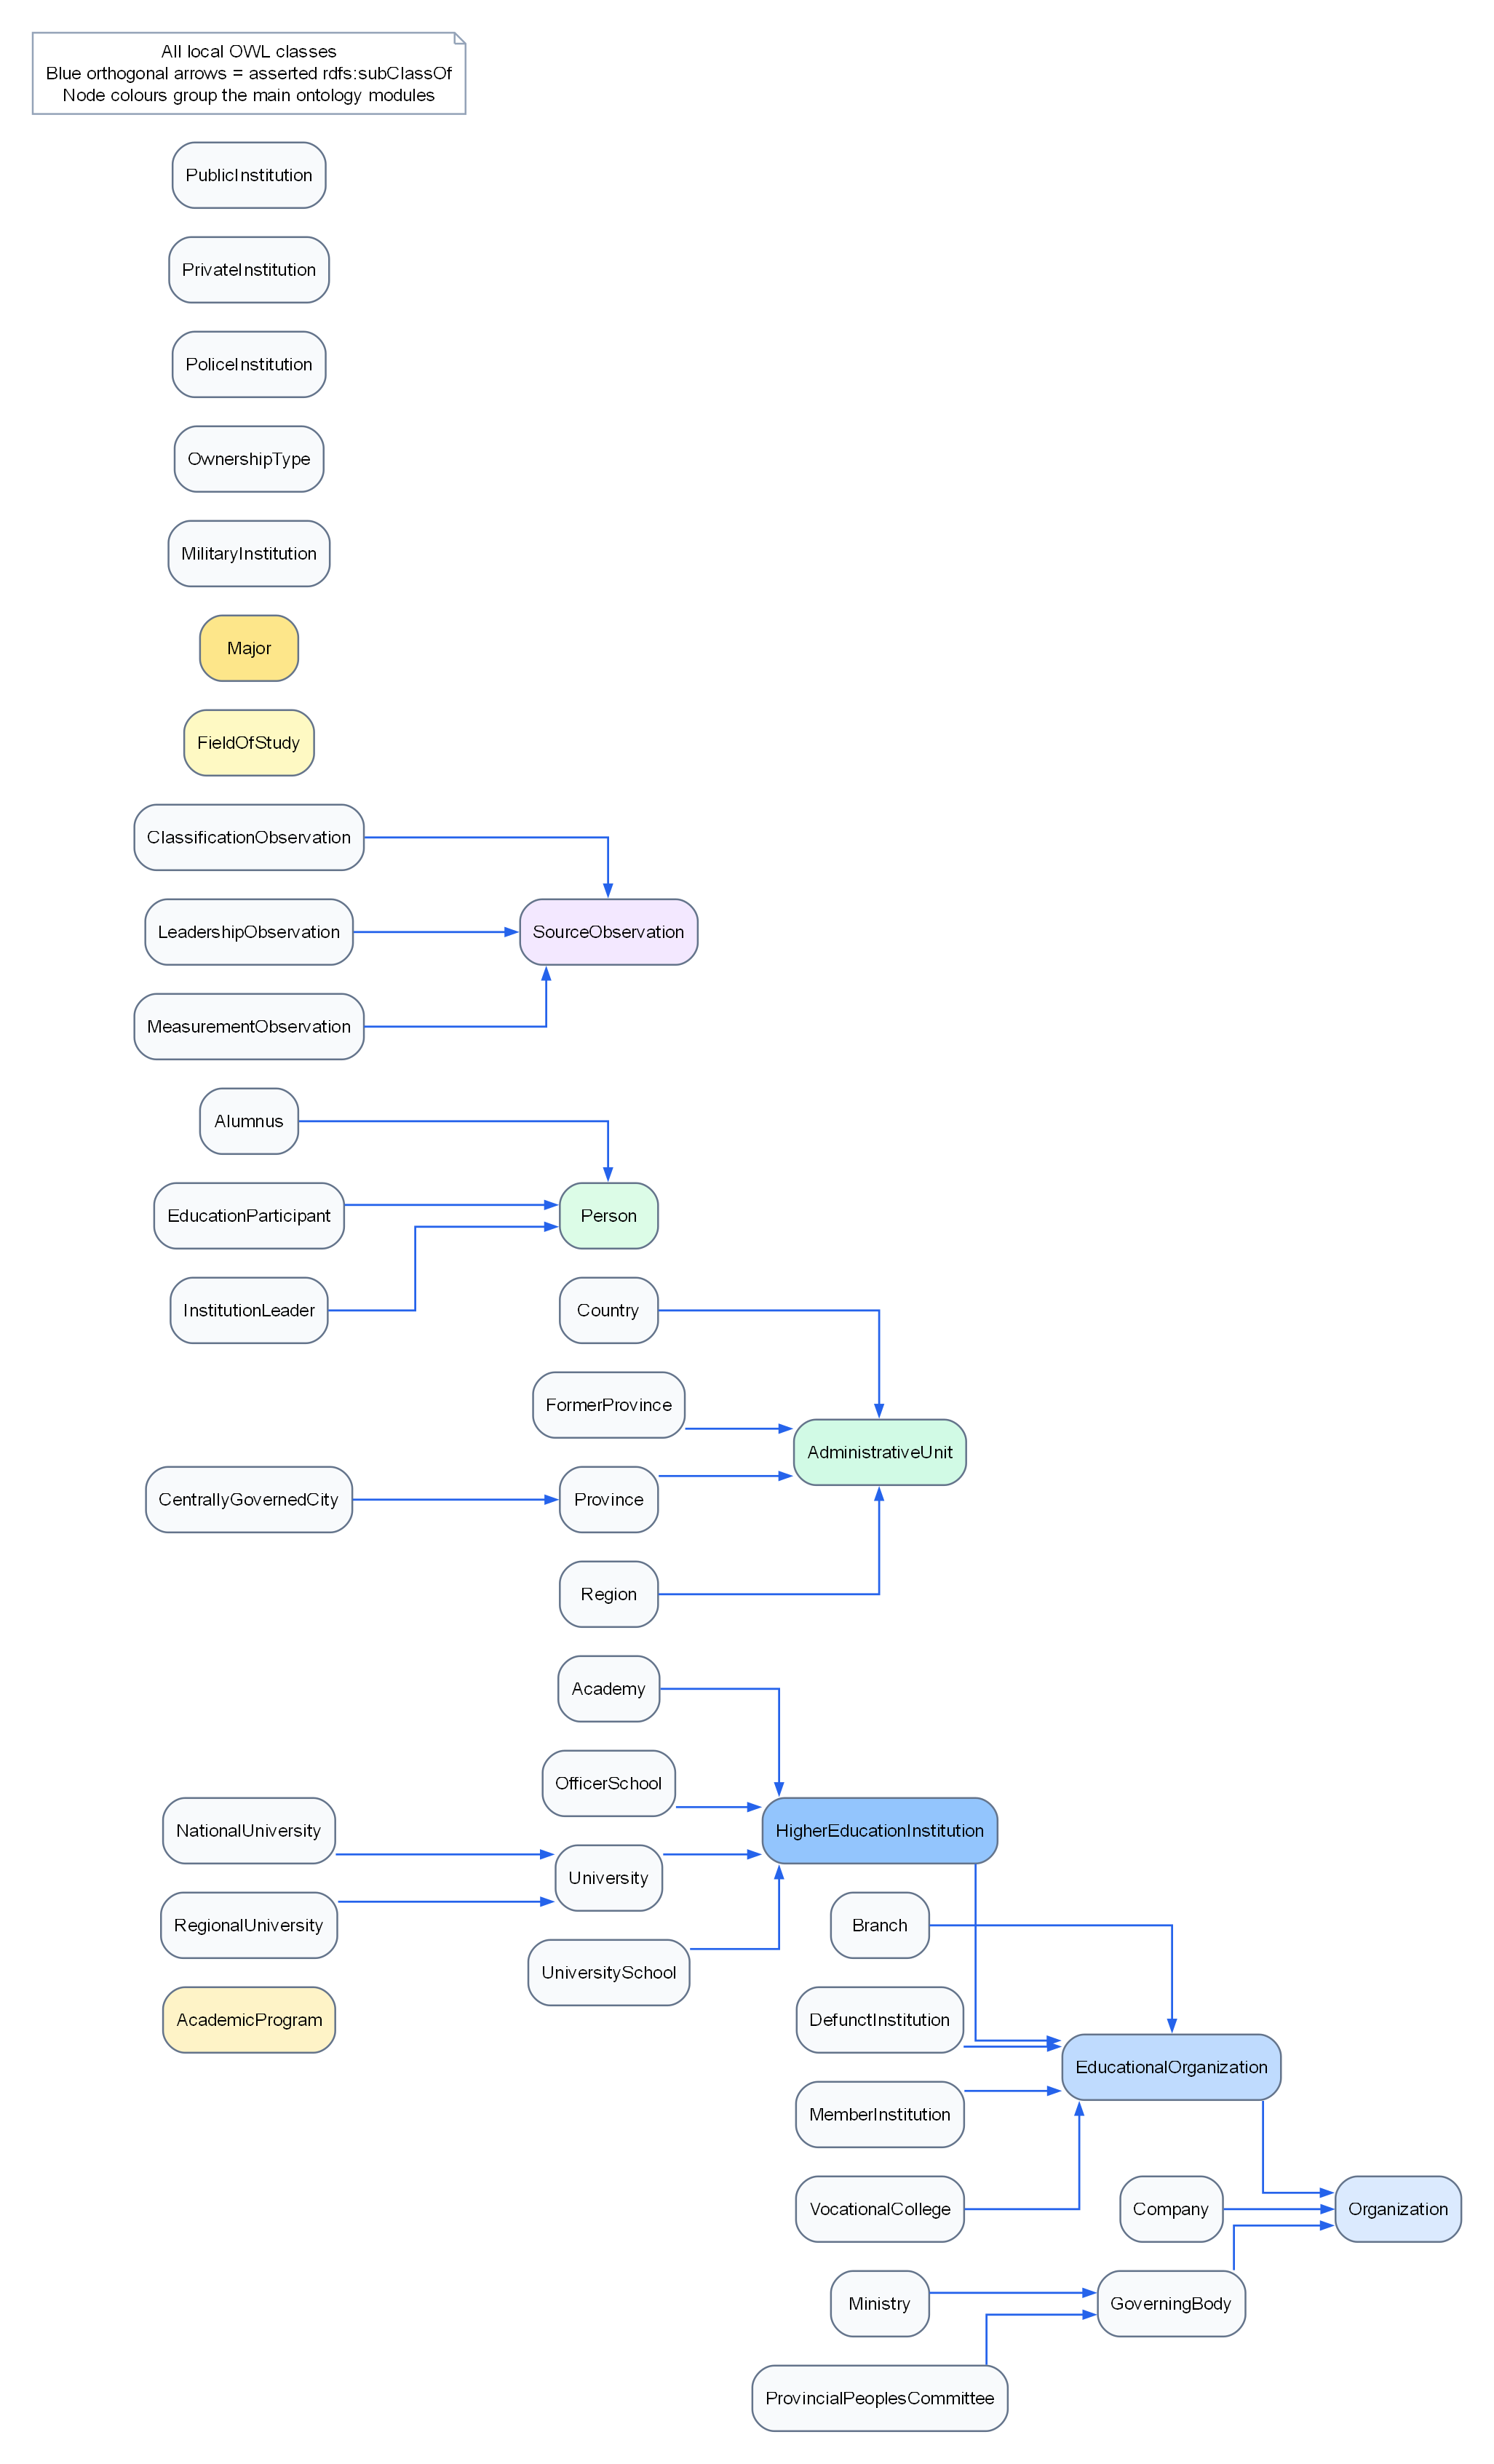
\includegraphics[width=\textwidth,height=0.84\textheight,keepaspectratio]{figures/ontology-tbox-hierarchy-clean.png}%
}
\caption[Complete local TBox class hierarchy]{Complete local OWL class hierarchy generated directly from \texttt{ontology/vnedu.ttl}. Every displayed blue arrow is an asserted \texttt{rdfs:subClassOf} triple; disconnected nodes are intentionally retained because the ontology does not assert a superclass for them. Orthogonal routing is used to avoid crossing edges.}\label{fig:tbox-hierarchy-clean}
\end{figure}

The hierarchy and the relation map answer different questions. A root class is not an OWL error under the open-world assumption: it is a class for which this ontology has not asserted a local superclass. In particular, \texttt{Person}, \texttt{AdministrativeUnit}, \texttt{AcademicProgram}, \texttt{FieldOfStudy}, \texttt{OwnershipType} and \texttt{SourceObservation} are independent modelling concepts. The defined classes \texttt{PublicInstitution}, \texttt{PrivateInstitution}, \texttt{MilitaryInstitution} and \texttt{PoliceInstitution} are classified by \texttt{owl:equivalentClass} restrictions rather than by an asserted \texttt{rdfs:subClassOf} edge; adding a superclass only to make a picture connected would change the semantics. If a future competency-questions review confirms that those categories are intended as direct kinds of educational organization, that axiom can be added with a test case; it is not inferred from the visualization requirement.

\clearpage
\begin{figure}[htbp]\centering
\IfFileExists{docs/report/figures/ontology-tbox-signatures-organization.png}{%
  \includegraphics[width=\textwidth,height=0.88\textheight,keepaspectratio]{docs/report/figures/ontology-tbox-signatures-organization.png}%
}{%
  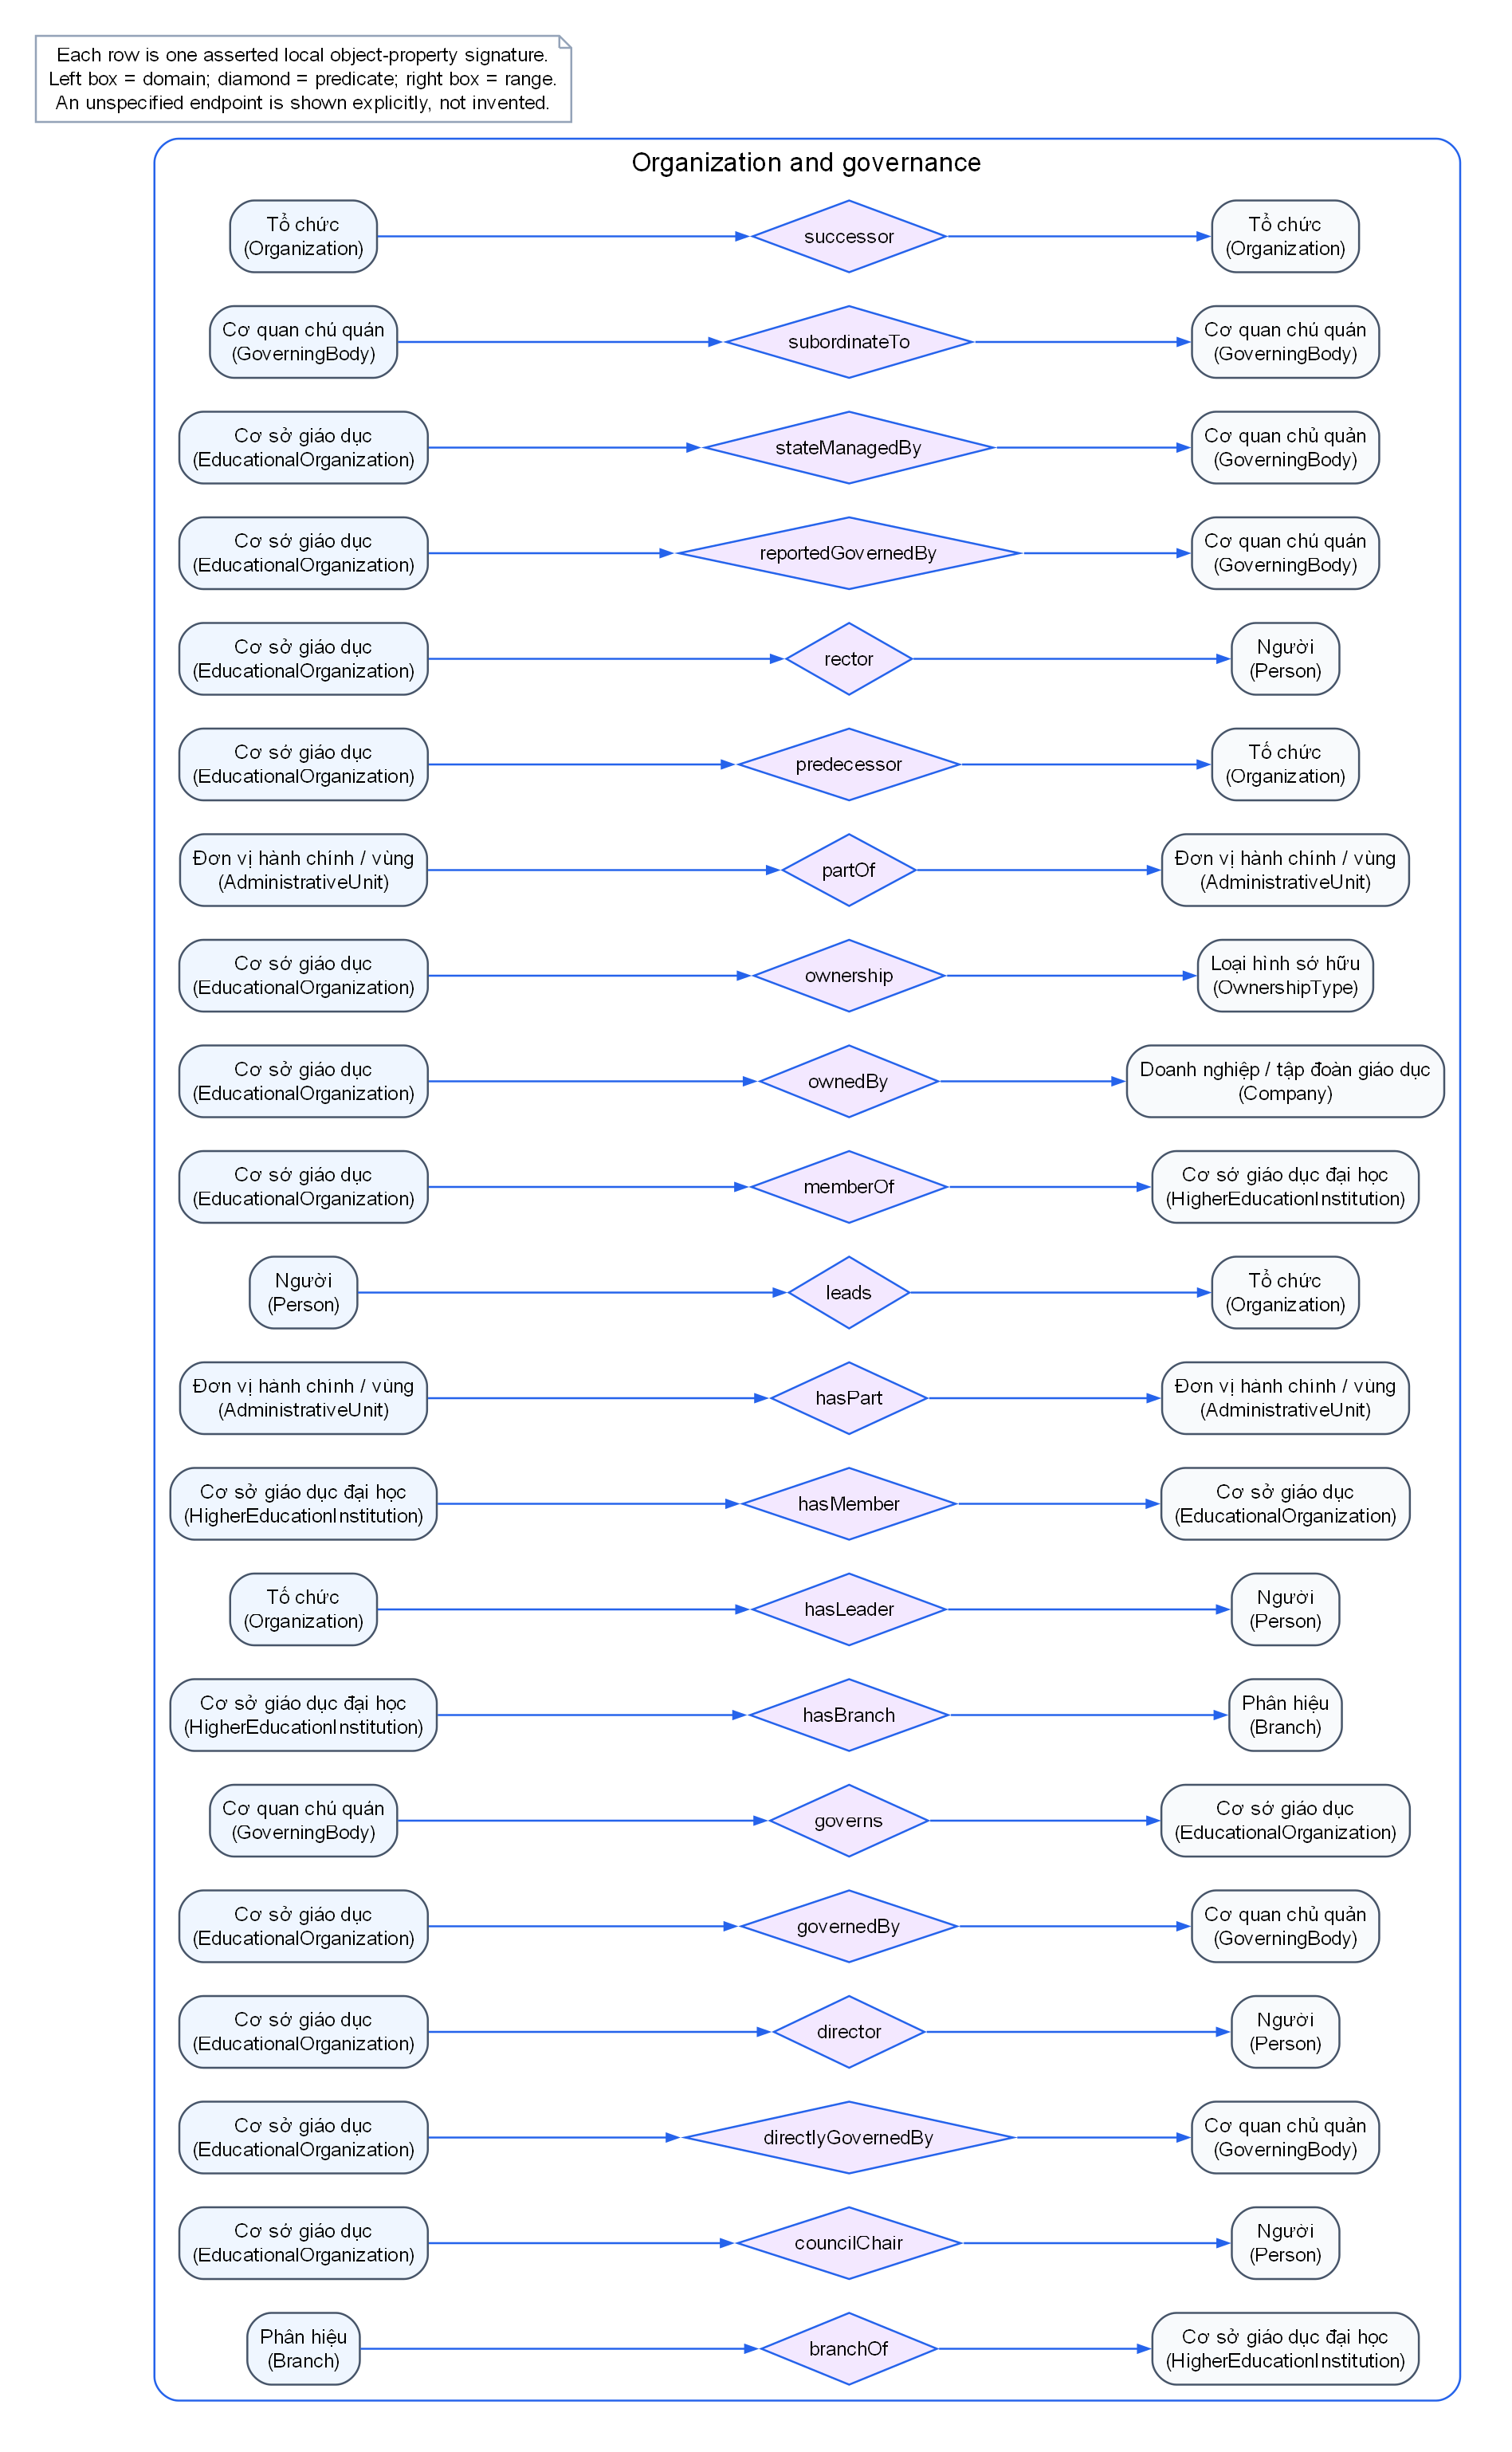
\includegraphics[width=\textwidth,height=0.88\textheight,keepaspectratio]{figures/ontology-tbox-signatures-organization.png}%
}
\caption[Organization and governance signatures]{Exact local object-property signatures for organization, governance, membership, ownership and structural relations. Each row is independent: left box is the declared domain, the diamond is the predicate, and right box is the declared range. No edge is routed through another row.}\label{fig:tbox-signatures-organization}
\end{figure}

\clearpage
\begin{figure}[htbp]\centering
\IfFileExists{docs/report/figures/ontology-tbox-signatures-education.png}{%
  \includegraphics[width=\textwidth,height=0.88\textheight,keepaspectratio]{docs/report/figures/ontology-tbox-signatures-education.png}%
}{%
  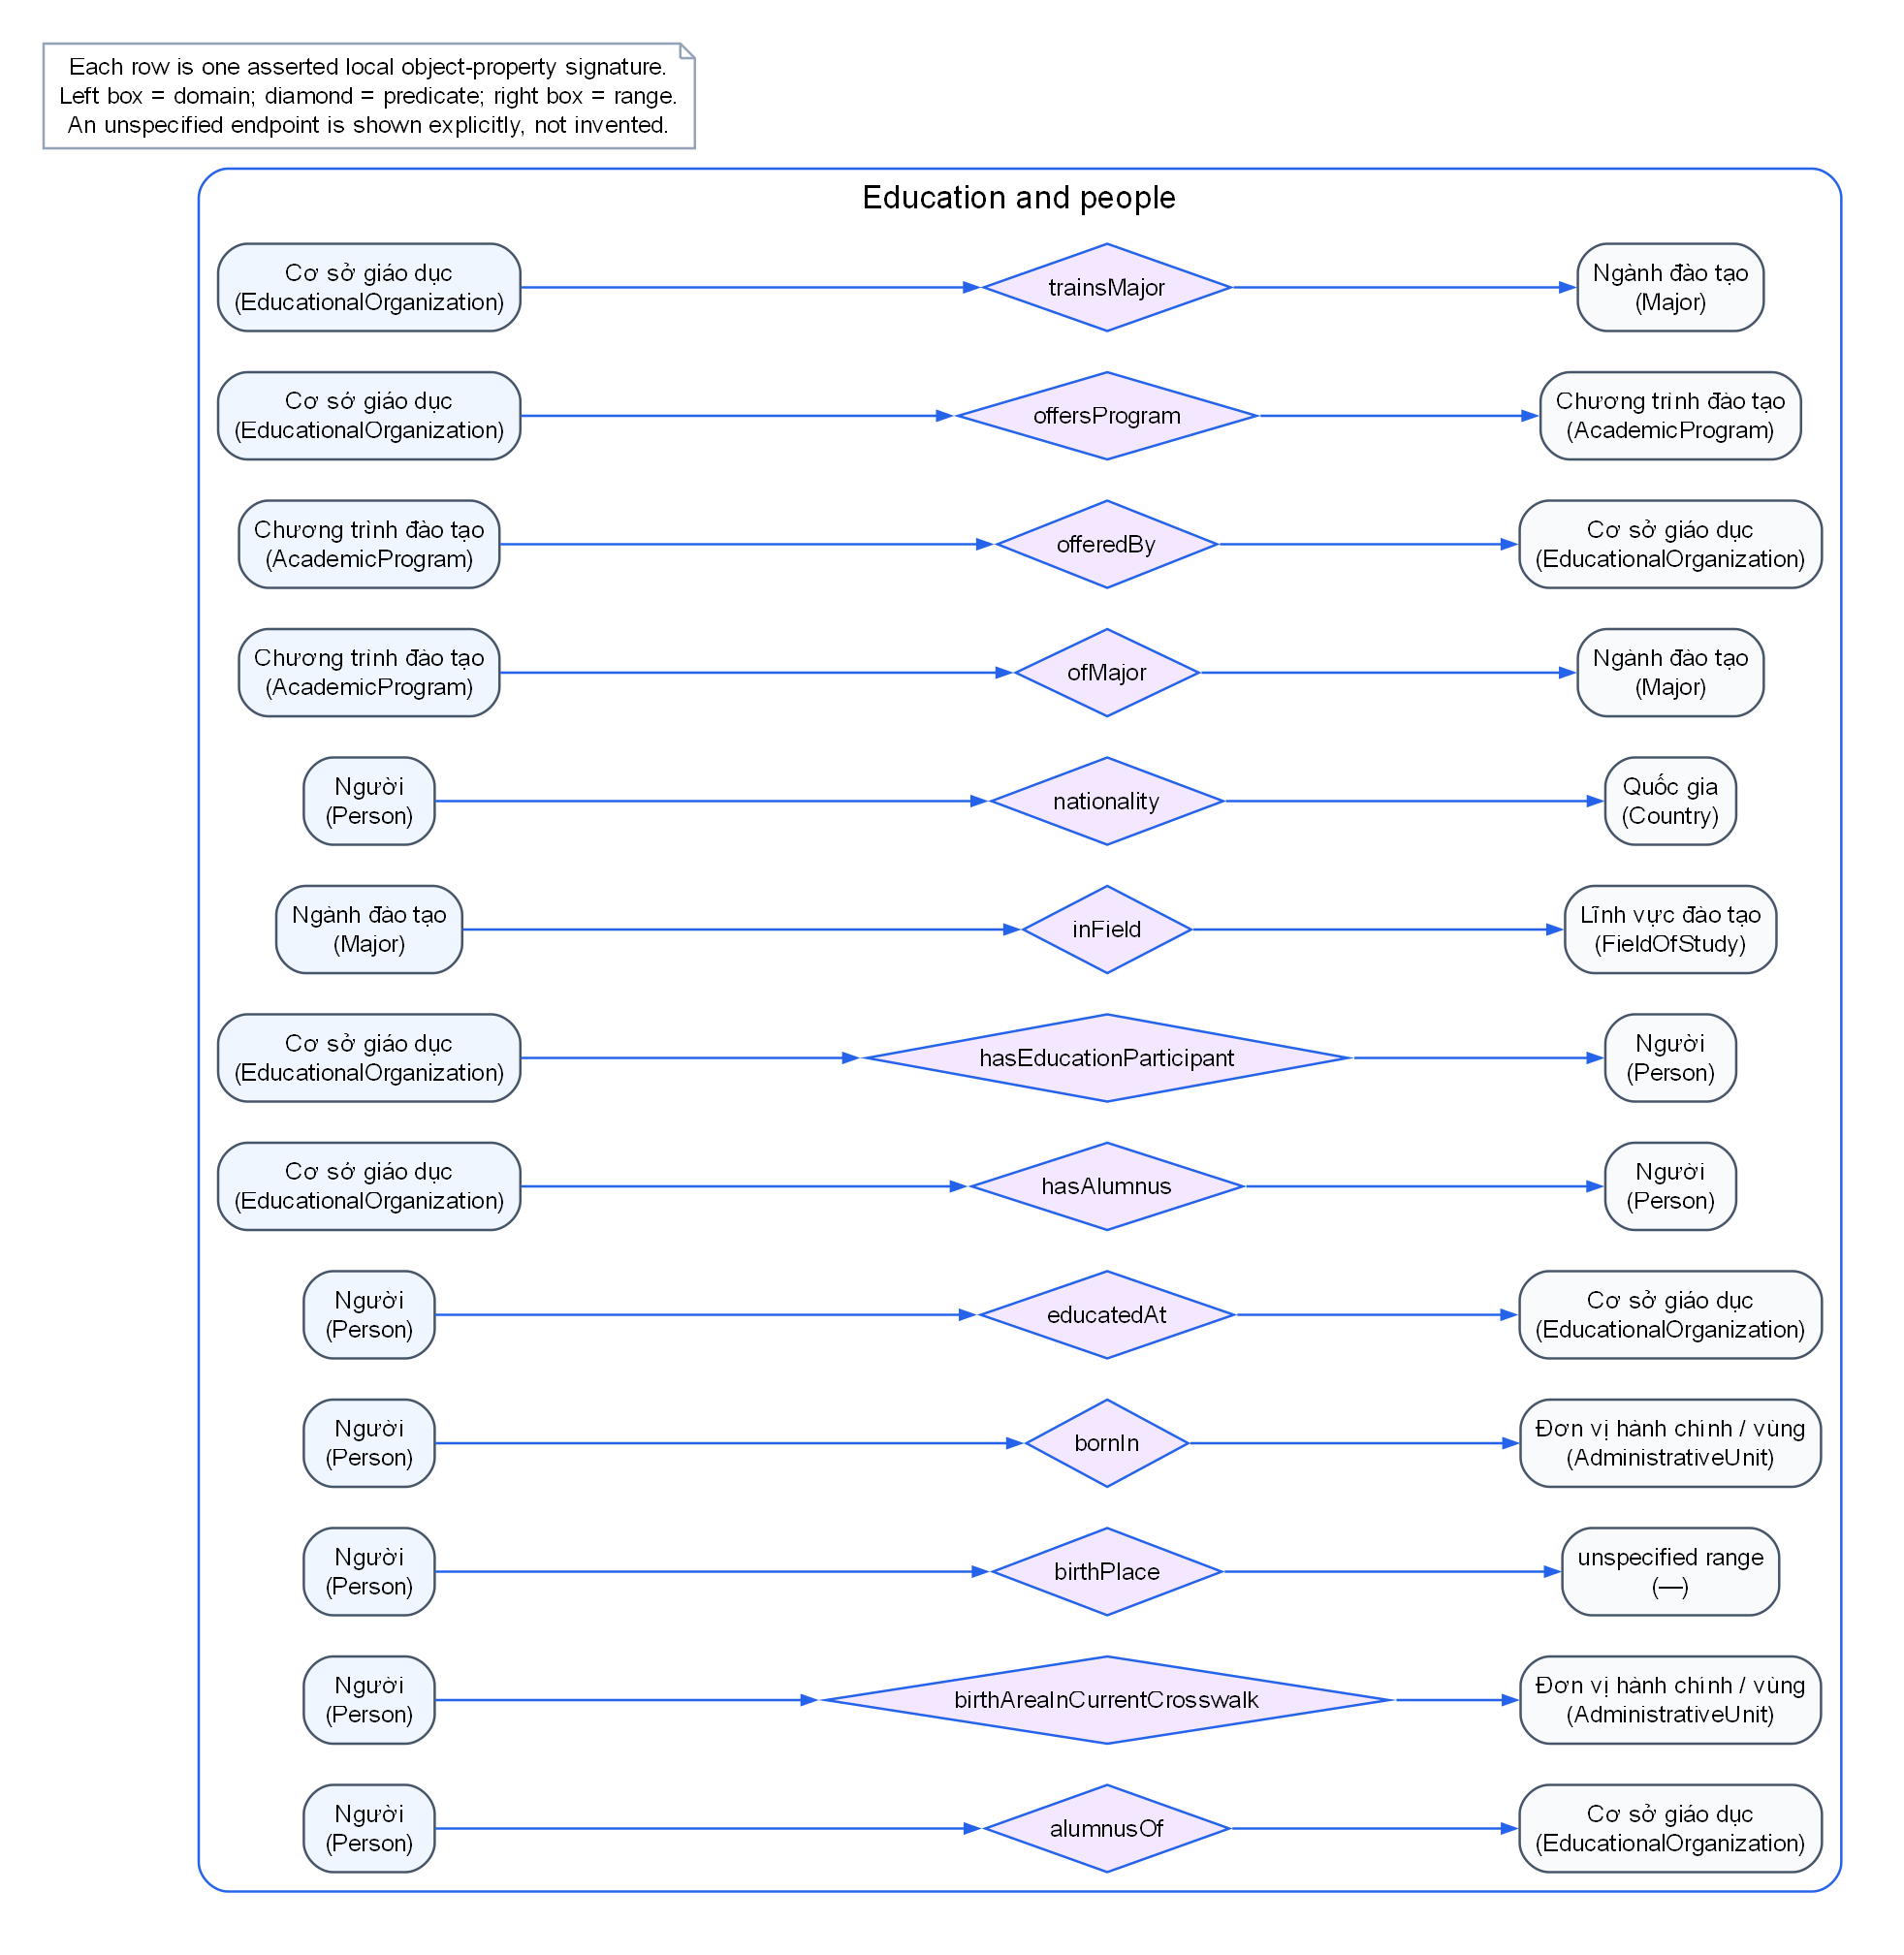
\includegraphics[width=\textwidth,height=0.88\textheight,keepaspectratio]{figures/ontology-tbox-signatures-education.png}%
}
\caption[Education and people signatures]{Exact local object-property signatures for programmes, majors, fields, people and educational participation. The missing range of \term{birthPlace} is shown explicitly as unspecified rather than guessed.}\label{fig:tbox-signatures-education}
\end{figure}

\clearpage
\begin{figure}[htbp]\centering
\IfFileExists{docs/report/figures/ontology-tbox-signatures-geography.png}{%
  \includegraphics[width=\textwidth,height=0.70\textheight,keepaspectratio]{docs/report/figures/ontology-tbox-signatures-geography.png}%
}{%
  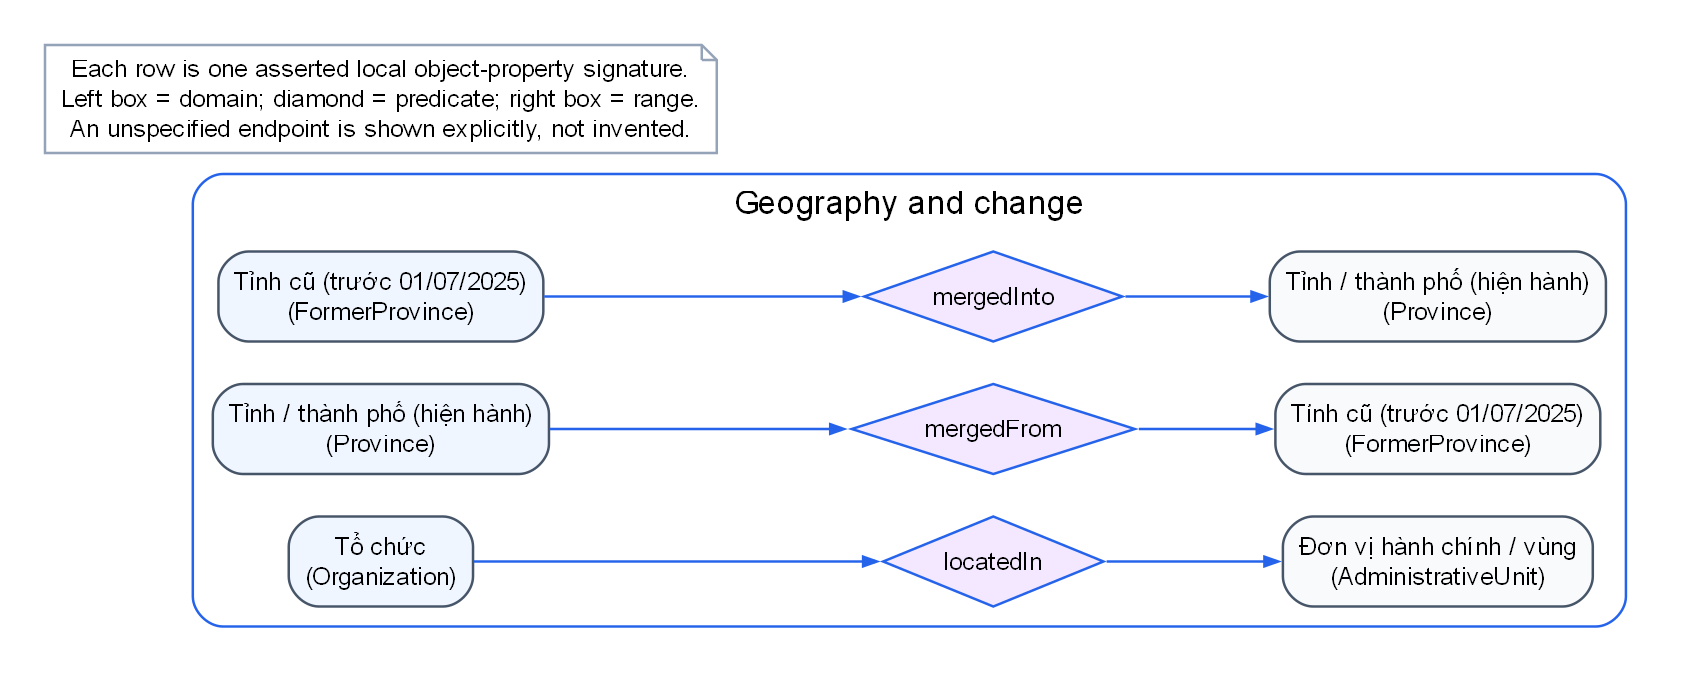
\includegraphics[width=\textwidth,height=0.70\textheight,keepaspectratio]{figures/ontology-tbox-signatures-geography.png}%
}
\caption[Geography and change signatures]{Exact local signatures for location and province-change relations. The former/current province distinction is represented as a directed relation, not as a timeless equivalence.}\label{fig:tbox-signatures-geography}
\end{figure}

\clearpage
\begin{figure}[htbp]\centering
\IfFileExists{docs/report/figures/ontology-tbox-signatures-other.png}{%
  \includegraphics[width=\textwidth,height=0.38\textheight,keepaspectratio]{docs/report/figures/ontology-tbox-signatures-other.png}%
}{%
  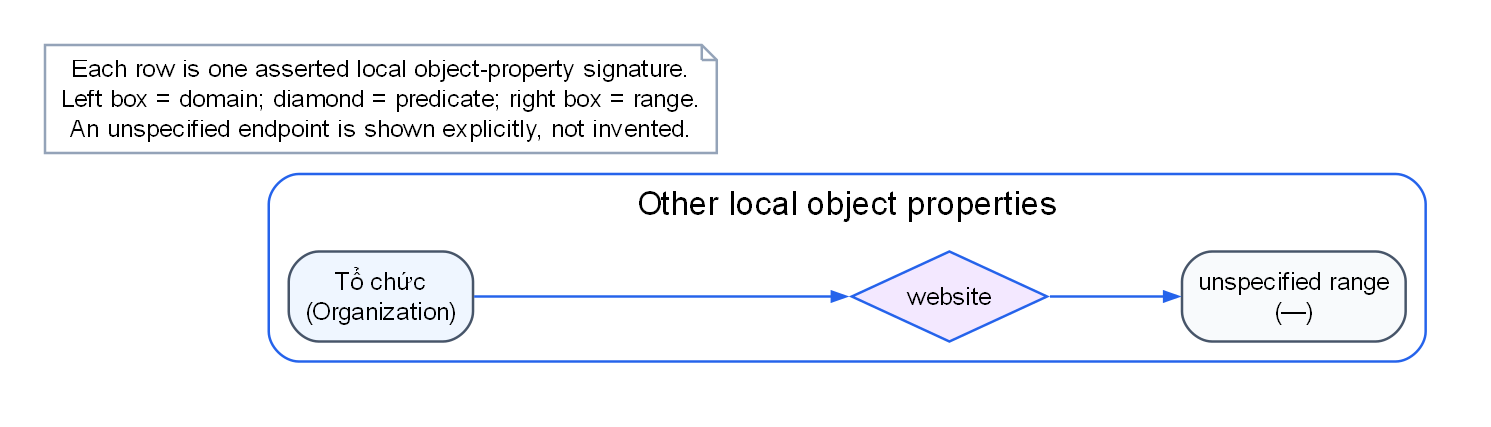
\includegraphics[width=\textwidth,height=0.38\textheight,keepaspectratio]{figures/ontology-tbox-signatures-other.png}%
}
\caption[Other local object-property signature]{The remaining local object property, \term{website}, has an asserted domain but no asserted range in the ontology. This is shown as an open endpoint, not silently assigned \texttt{xsd:anyURI}.}\label{fig:tbox-signatures-other}
\end{figure}

\clearpage
\begin{figure}[htbp]\centering
\IfFileExists{docs/report/figures/abox-instance-neighborhood.png}{%
  \includegraphics[width=\textwidth,height=0.72\textheight,keepaspectratio]{docs/report/figures/abox-instance-neighborhood.png}%
}{%
  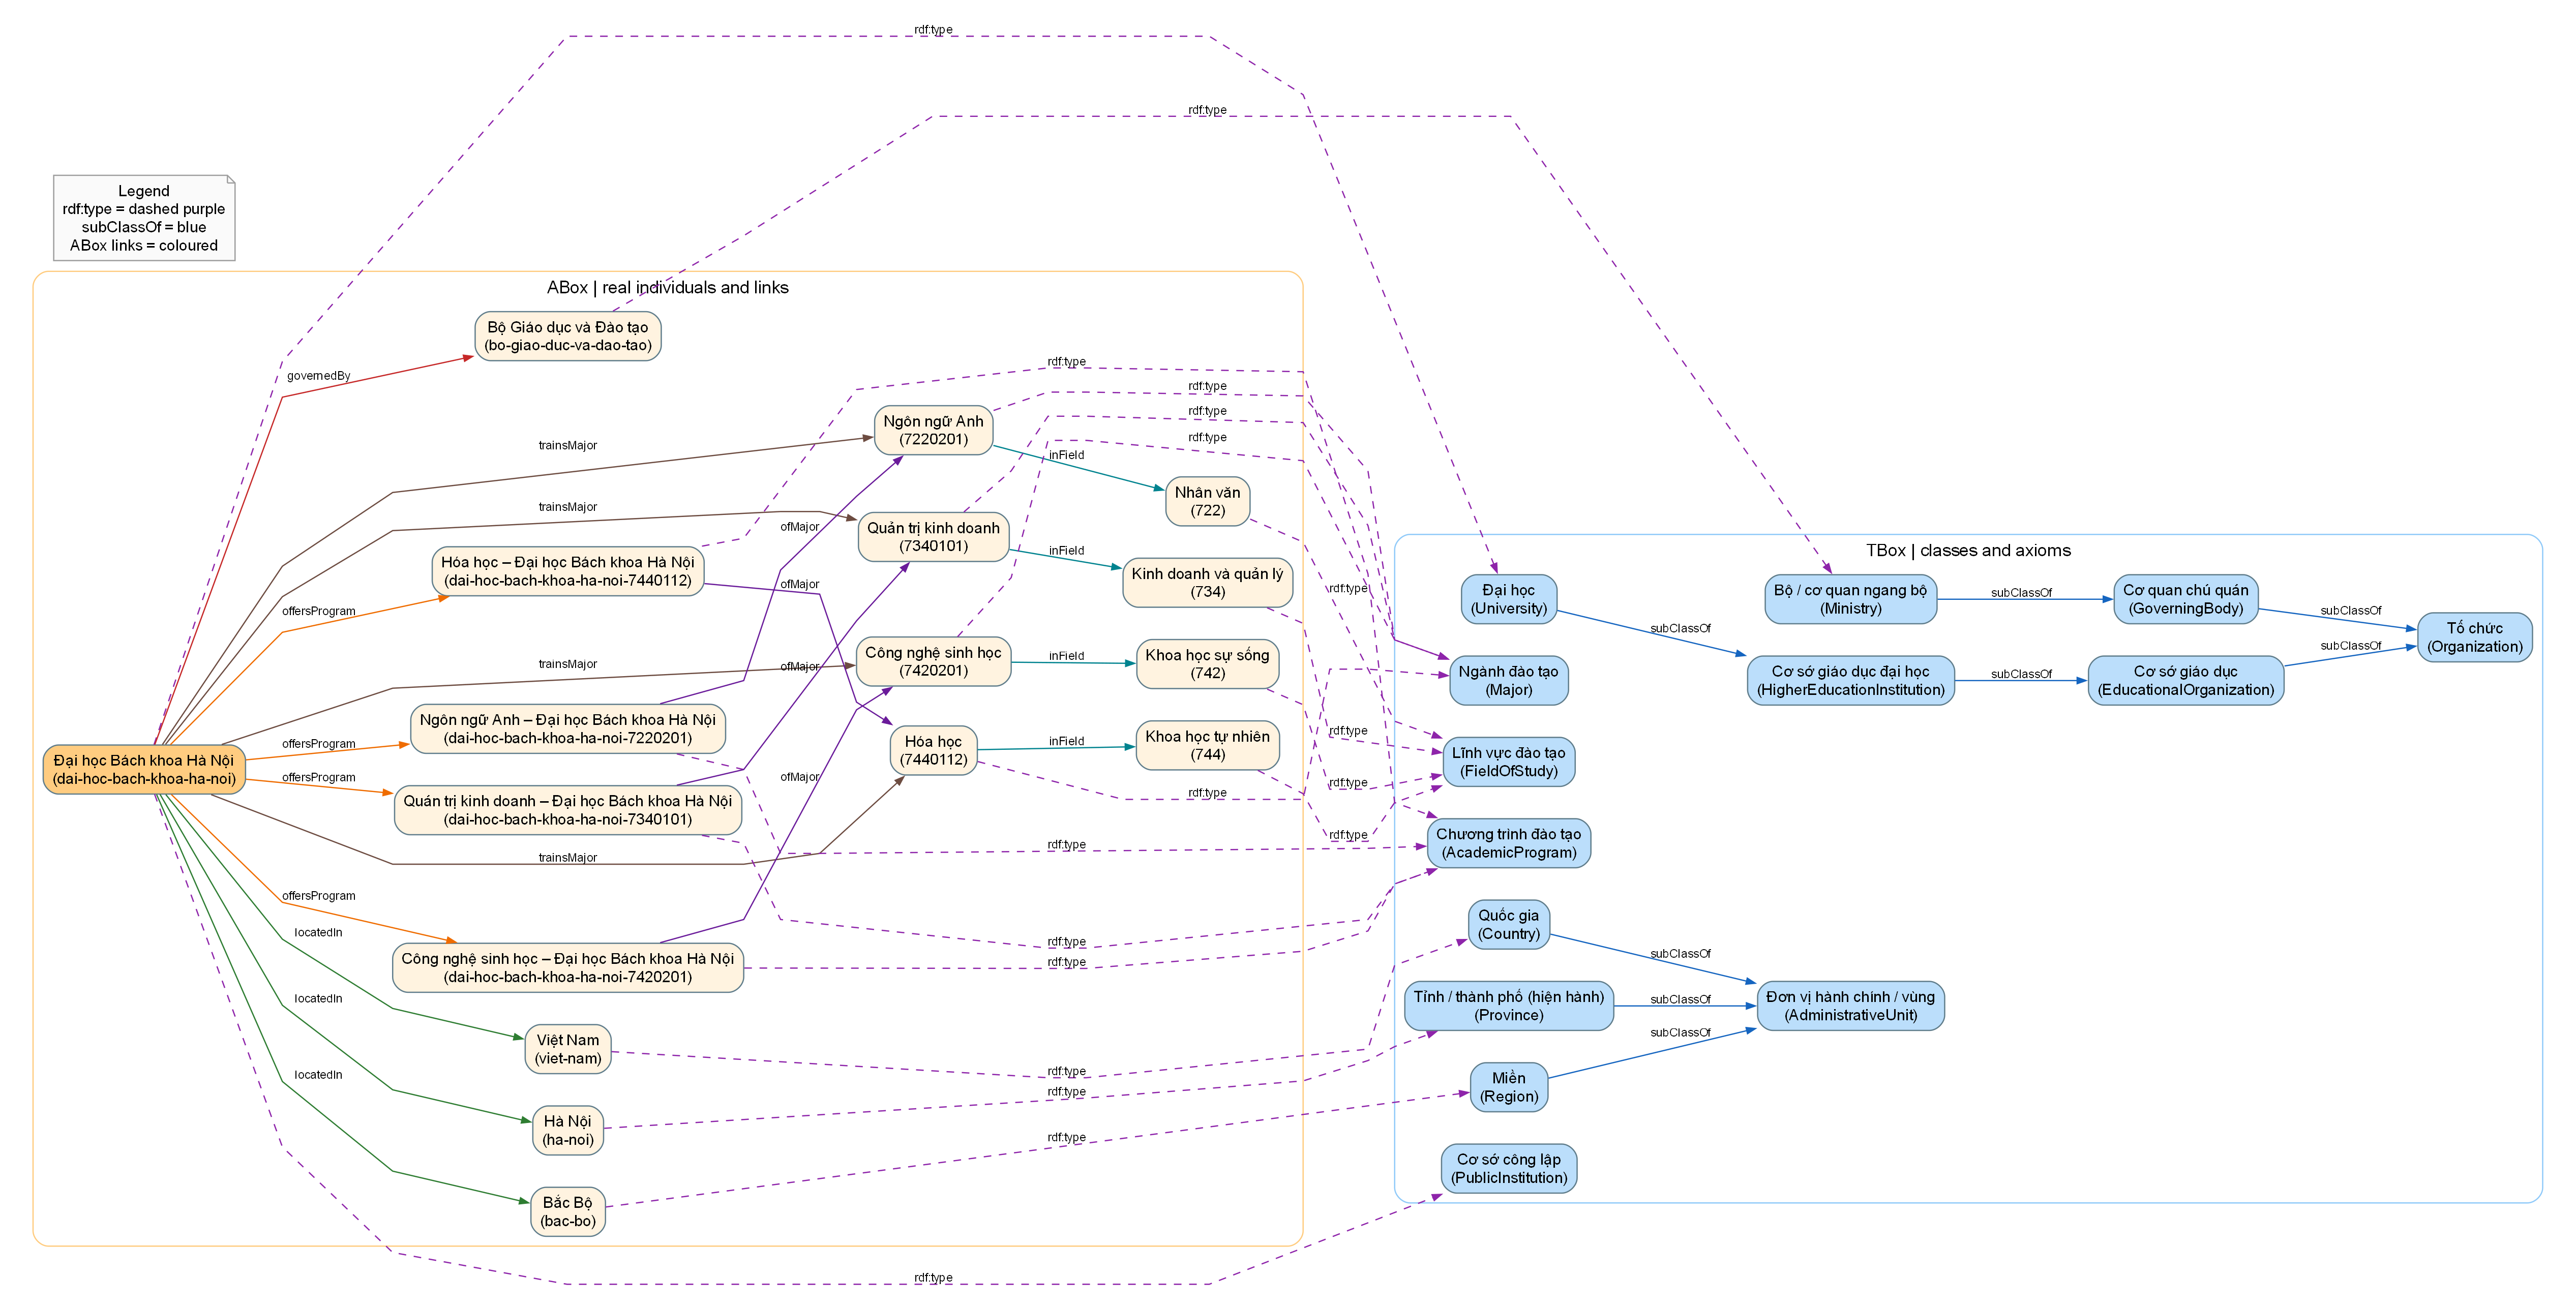
\includegraphics[width=\textwidth,height=0.72\textheight,keepaspectratio]{figures/abox-instance-neighborhood.png}%
}
\caption[ABox instance neighborhood for a real university]{Data-driven ABox view generated from the gold serving union. The orange nodes are named individuals: one university, four programmes, four majors, four fields, location units and the reported governing body. Coloured edges are asserted or materialized object-property links; dashed \texttt{rdf:type} edges connect only the most specific visible types to the TBox. This reproducible instance view complements the main unique-node TBox map and the direct Protégé inspection.}\label{fig:abox-instance-neighborhood}
\end{figure}
\clearpage

\subsection{TBox, ABox and constraint semantics}
The ontology is intentionally split into a schema layer and a data layer. The TBox is
\texttt{ontology/vnedu.ttl}: classes, subclass axioms, property signatures, inverse properties,
property chains, defined classes and selected disjointness. The ABox is the generated RDF in
\texttt{data/gold/vnedu-data.ttl}, with \texttt{data/gold/vnedu-all.ttl} as the serving union of
asserted data and materialized entailments. A URI such as
\texttt{university:dai-hoc-bach-khoa-ha-noi} is an individual; \texttt{vnedu:University} and
\texttt{vnedu:HigherEducationInstitution} are classes. Mixing these levels without explicit
\texttt{rdf:type} and \texttt{rdfs:subClassOf} labels is what made the earlier graph misleading.

\begin{longtable}{P{3.4cm}P{6.2cm}P{5.0cm}}
\caption{Separation of ontology axioms, data assertions and validation constraints.}\label{tab:tbox-abox-constraints}\\
\toprule Layer & What is asserted & Correct interpretation \\\midrule\endfirsthead
\toprule Layer & What is asserted & Correct interpretation \\\midrule\endhead
TBox & \texttt{rdfs:subClassOf}, \texttt{rdfs:domain}, \texttt{rdfs:range}, inverses, chains, restrictions and disjointness. & Schema-level meaning and inference rules; it does not require every possible individual to have every field. \\
ABox & Individuals, \texttt{rdf:type}, object-property links, literals, external identifiers and provenance observations. & Source-backed claims; an omitted triple is unknown under the open-world assumption. \\
OWL reasoning & Domain/range and property axioms materialize types and consequences, including inferred superclasses and inverse links. & A wrong domain/range can infer a wrong type; OWL entailment is not a database foreign-key rejection. \\
SHACL & \texttt{shapes/vnedu-shapes.ttl} checks cardinality, datatypes, patterns, temporal intervals and observation structure. & Closed-world data-quality validation, separate from OWL entailments. \\
\bottomrule
\end{longtable}

The design therefore uses domain and range as semantic typing constraints, and SHACL for operational
requirements such as ``at least one provider'' or a valid year range. This is the standards-correct
combination for an RDF/OWL knowledge graph: imposing every relational-database NOT NULL or foreign-key
rule directly in OWL would be unsound under the open-world assumption. Time-dependent legal categories
remain qualified observations rather than permanent global disjointness axioms.

\begin{figure}[htbp]\centering
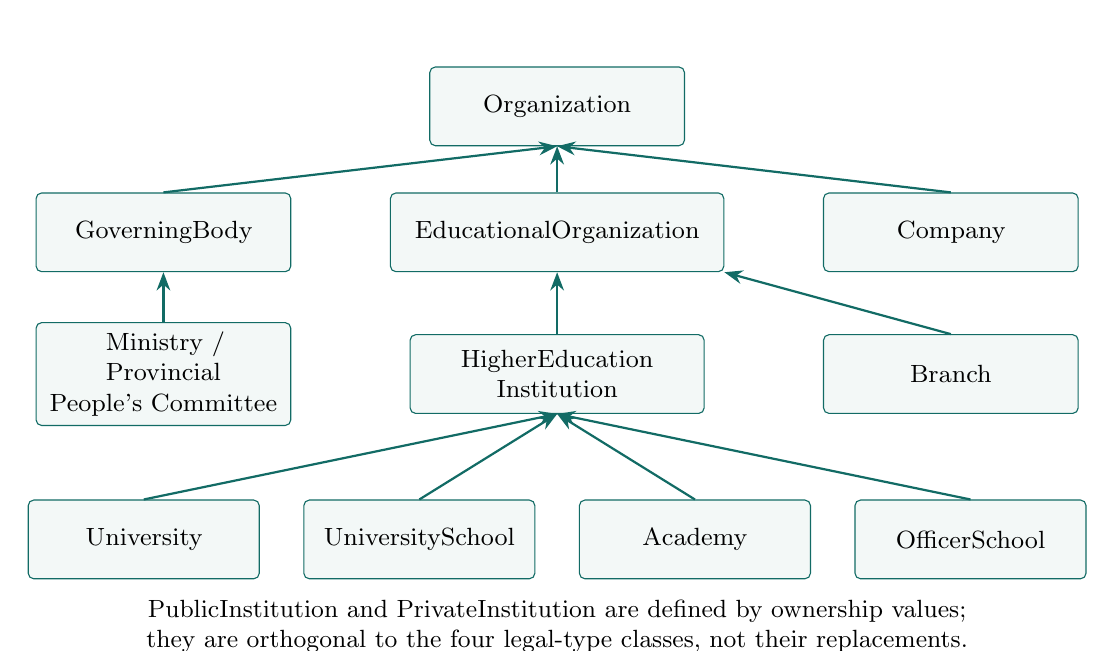
\begin{tikzpicture}
\node[auditbox] (org) at (0,0) {Organization};
\node[auditbox] (body) at (-5,-1.6) {GoverningBody};
\node[auditbox,text width=4cm] (edu) at (0,-1.6) {EducationalOrganization};
\node[auditbox] (company) at (5,-1.6) {Company};
\node[auditbox,text width=3.5cm] (hei) at (0,-3.4) {HigherEducation\\Institution};
\node[auditbox] (branch) at (5,-3.4) {Branch};
\node[auditbox] (min) at (-5,-3.4) {Ministry / Provincial\\People's Committee};
\node[auditbox,text width=2.7cm] (u) at (-5.25,-5.5) {University};
\node[auditbox,text width=2.7cm] (s) at (-1.75,-5.5) {UniversitySchool};
\node[auditbox,text width=2.7cm] (a) at (1.75,-5.5) {Academy};
\node[auditbox,text width=2.7cm] (o) at (5.25,-5.5) {OfficerSchool};
\foreach \n in {body,edu,company} \draw[auditarr] (\n.north)--(org.south);
\draw[auditarr] (hei)--(edu);
\draw[auditarr] (branch.north)--(edu.south east);
\draw[auditarr] (min)--(body);
\foreach \n in {u,s,a,o} \draw[auditarr] (\n.north)--(hei.south);
\node[font=\small,align=center] at (0,-6.6) {PublicInstitution and PrivateInstitution are defined by ownership values;\\they are orthogonal to the four legal-type classes, not their replacements.};
\end{tikzpicture}

\caption[Organizational class hierarchy]{Selected organizational hierarchy. Arrows point from subclass to superclass.
The four legal-type classes are no longer globally disjoint: an enduring institution can change type.
This is a selected view of \metricClasses{} classes.}\label{fig:taxonomy}
\end{figure}
\begin{figure}[htbp]\centering
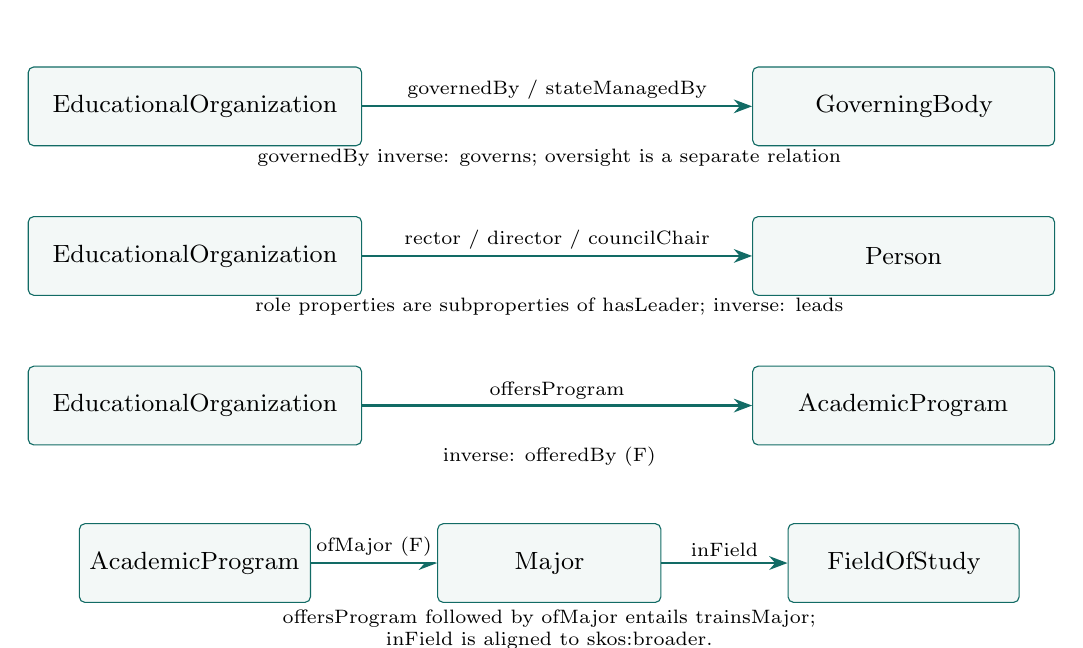
\begin{tikzpicture}
\node[auditbox,text width=4cm] (e1) at (0,0) {EducationalOrganization};
\node[auditbox,text width=3.6cm] (g) at (9,0) {GoverningBody};
\draw[auditarr] (e1)--node[auditlabel,above]{governedBy / stateManagedBy}(g);
\node[font=\scriptsize] at (4.5,-0.65) {governedBy inverse: governs; oversight is a separate relation};
\node[auditbox,text width=4cm] (e2) at (0,-1.9) {EducationalOrganization};
\node[auditbox,text width=3.6cm] (p) at (9,-1.9) {Person};
\draw[auditarr] (e2)--node[auditlabel,above]{rector / director / councilChair}(p);
\node[font=\scriptsize] at (4.5,-2.55) {role properties are subproperties of hasLeader; inverse: leads};
\node[auditbox,text width=4cm] (e3) at (0,-3.8) {EducationalOrganization};
\node[auditbox,text width=3.6cm] (prog) at (9,-3.8) {AcademicProgram};
\draw[auditarr] (e3)--node[auditlabel,above]{offersProgram}(prog);
\node[font=\scriptsize] at (4.5,-4.45) {inverse: offeredBy (F)};
\node[auditbox,text width=2.7cm] (pr2) at (0,-5.8) {AcademicProgram};
\node[auditbox,text width=2.6cm] (major) at (4.5,-5.8) {Major};
\node[auditbox,text width=2.7cm] (field) at (9,-5.8) {FieldOfStudy};
\draw[auditarr] (pr2)--node[auditlabel,above]{ofMajor (F)}(major);
\draw[auditarr] (major)--node[auditlabel,above]{inField}(field);
\node[font=\scriptsize,align=center] at (4.5,-6.65) {offersProgram followed by ofMajor entails trainsMajor;\\inField is aligned to skos:broader.};
\end{tikzpicture}

\caption[Property signatures across ontology modules]{Selected domain--property--range signatures.
These arrows are not mandatory foreign keys. Program providers and majors are no longer functional:
multiple values must not force different institutions or subjects to become identical.}\label{fig:relations}
\end{figure}
\begin{figure}[htbp]\centering
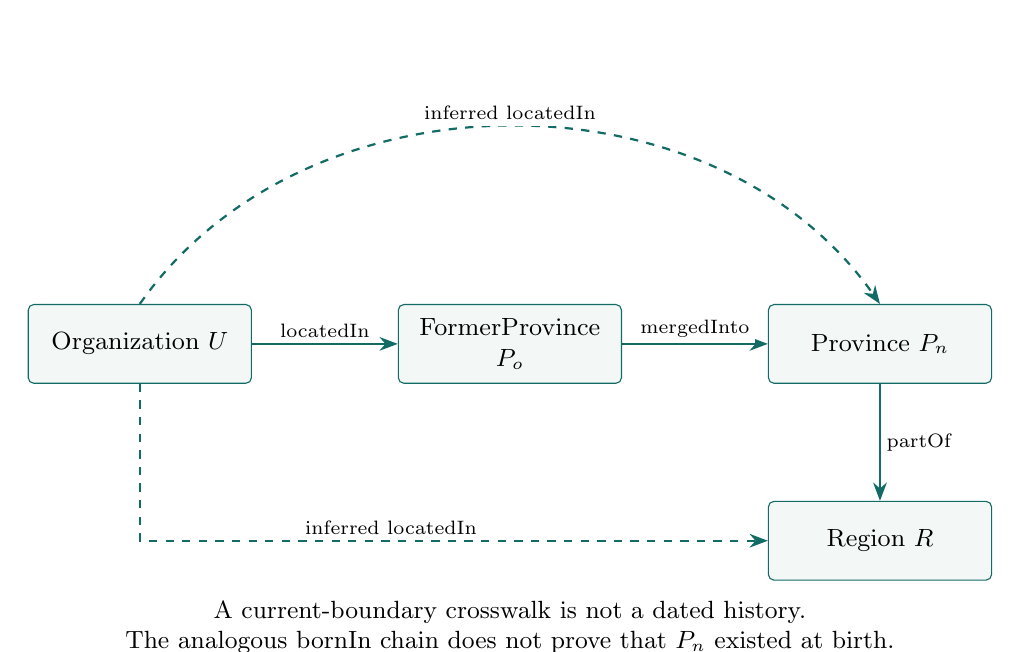
\begin{tikzpicture}
\node[auditbox,text width=2.6cm] (u) at (0,0) {Organization $U$};
\node[auditbox,text width=2.6cm] (old) at (4.7,0) {FormerProvince\\$P_o$};
\node[auditbox,text width=2.6cm] (new) at (9.4,0) {Province $P_n$};
\node[auditbox,text width=2.6cm] (region) at (9.4,-2.5) {Region $R$};
\draw[auditarr] (u)--node[auditlabel,above]{locatedIn}(old);
\draw[auditarr] (old)--node[auditlabel,above]{mergedInto}(new);
\draw[auditarr] (new)--node[auditlabel,right]{partOf}(region);
\draw[auditarr,dashed] (u.north) to[out=55,in=125] node[auditlabel,above]{inferred locatedIn} (new.north);
\draw[auditarr,dashed] (u.south)|-node[auditlabel,pos=0.7,above]{inferred locatedIn}(region.west);
\node[font=\small,align=center] at (4.7,-3.6) {A current-boundary crosswalk is not a dated history.\\The analogous bornIn chain does not prove that $P_n$ existed at birth.};
\end{tikzpicture}

\caption[Geographic property-chain inference]{Institution-location inference under the selected administrative
crosswalk. It does not establish historical validity. Birth-area mapping now uses a separate
\term{birthAreaInCurrentCrosswalk} predicate instead of adding historical \term{bornIn} statements.}\label{fig:geo-chain}
\end{figure}

\subsection{Implemented corrections and evidence limits}
The design is standards-based and suitable for an educational knowledge-graph prototype,
but consistency is not a certificate of factual accuracy. Version 2.2 makes the following
changes without reminting existing entity identifiers.
{\small
\begin{longtable}{P{3.7cm}P{6.1cm}P{4.8cm}}
\caption{Ontology 2.2 corrections and their limits.}\label{tab:design-review}\\
\toprule Concern & Implemented correction & Evidence boundary \\\midrule\endfirsthead
\toprule Concern & Implemented correction & Evidence boundary \\\midrule\endhead
Supervision versus inclusion &
Removed parent-organization alignments from governance, subordination, ownership and membership. The branch alignment remains because a branch is a structural subdivision. &
Supervision or investment does not automatically establish organizational parenthood. \\
Direct versus indirect governance &
Added \term{directlyGovernedBy} and \term{reportedGovernedBy} under the broad \term{governedBy}; only the broad relation propagates through superiors. &
Legacy source relations migrate to reported, not unsupported direct, governance. \\
Leadership versus employment &
Removed leader-to-employee and leader-to-\term{worksFor} alignments; added role observations. &
A council chair need not be an employee. \\
Institutional type changes &
Removed global disjointness between the four legal-type classes; added classification observations. &
The class projection is not a dated authoritative legal register. \\
Education versus alumni &
Recorded education becomes \term{educatedAt}, with the neutral inferred class \term{EducationParticipant}. &
Attendance does not entail graduation. Alumni terms remain for explicit evidence. \\
Joint programs &
Removed functionality from \term{offeredBy} and \term{ofMajor}; SHACL requires at least one provider and major. &
Curated program identifiers still do not distinguish all curriculum variants. \\
Birth geography &
Successor and containment chains produce \term{birthAreaInCurrentCrosswalk}, not additional \term{bornIn} facts. &
A current province is not asserted to have existed at birth. \\
Version publication &
Archived 2.1 and 2.2 Turtle; generated HTML, Turtle and JSON-LD version documents and dynamic routes. &
The source and Pages workflow provide the route; stable public uptime still depends on deployment. \\
\bottomrule
\end{longtable}}

\subsection{Standards and conformance assessment}
The audited ontology follows the RDF 1.1/Turtle and OWL 2 RDF serialisation conventions and
uses explicit OWL classes, object properties, datatype properties, inverse properties,
selected functional properties, disjointness, property chains and defined classes. The
current source contains \metricClasses{} local classes, \metricObjectProperties{} local object
properties, \metricDataProperties{} local datatype properties and \metricOntologyTriples{} ontology triples.
The visualisation above is generated from those current source counts, so it can be regenerated
after an ontology change rather than becoming a stale hand-drawn figure.

The design is suitable for a standards-based academic prototype, but it is not an automatic
``five-star'' certification. The following claims are deliberately separated:
\begin{longtable}{P{4.0cm}P{5.6cm}P{5.0cm}}
\caption{Standards assessment and remaining boundaries.}\label{tab:standards-assessment}\\
\toprule Area & Evidence in this release & Honest qualification \\\midrule\endfirsthead
\toprule Area & Evidence in this release & Honest qualification \\\midrule\endhead
RDF and URI design & Stable HTTPS namespace, version IRI, Turtle/JSON-LD/N-Triples publication, content negotiation checks and licence metadata. & Deployment and long-term availability at the canonical origin remain operational responsibilities. \\
OWL 2 modelling & The ontology parses as RDF and passes the OWL API \texttt{OWL2RLProfile} gate with zero violations; inverse relations, chains, restrictions, equivalent classes and selected disjointness remain explicit. & This certifies profile membership of the local ontology, not complete imported-vocabulary semantics or factual correctness. \\
Constraint validation & SHACL shapes validate required fields, datatypes, temporal intervals and observation structure; the current suite reports zero violations under its policy. & Warnings reflect incomplete source coverage; SHACL validation is not proof of factual truth. \\
Provenance and time & PROV-O-style source links and reified evidence observations preserve snapshot context and optional temporal qualifiers. & The current Silver snapshot still lacks claim-level dates for many facts; an undated observation is not a current fact. \\
Vocabulary reuse & Conservative links to Schema.org, FOAF, DBpedia, SKOS, PROV-O and external identifiers. & External ontologies are not fully imported and reasoned over; alignments must remain semantically narrow. \\
Linked Data stars & Machine-readable publication, stable links, external links, licence and open formats are implemented. & The five-star scheme is a publication maturity heuristic, not a formal conformance test, and does not certify accuracy, security or production performance. \\
\bottomrule
\end{longtable}

\subsection{Qualified observations and temporal interpretation}
The transformer creates \metricObservations{} \term{SourceObservation} records, including
leadership, measurement and classification specializations. Each reifies a triple through
\term{rdf:subject}, \term{rdf:predicate} and \term{rdf:object}. Its SHA-256-derived URI includes
the assertion, snapshot digest, source context and qualifiers. Identical evidence preserves
the observation URI; changed evidence creates a different record. Entity URIs remain stable.

\begin{figure}[htbp]\centering
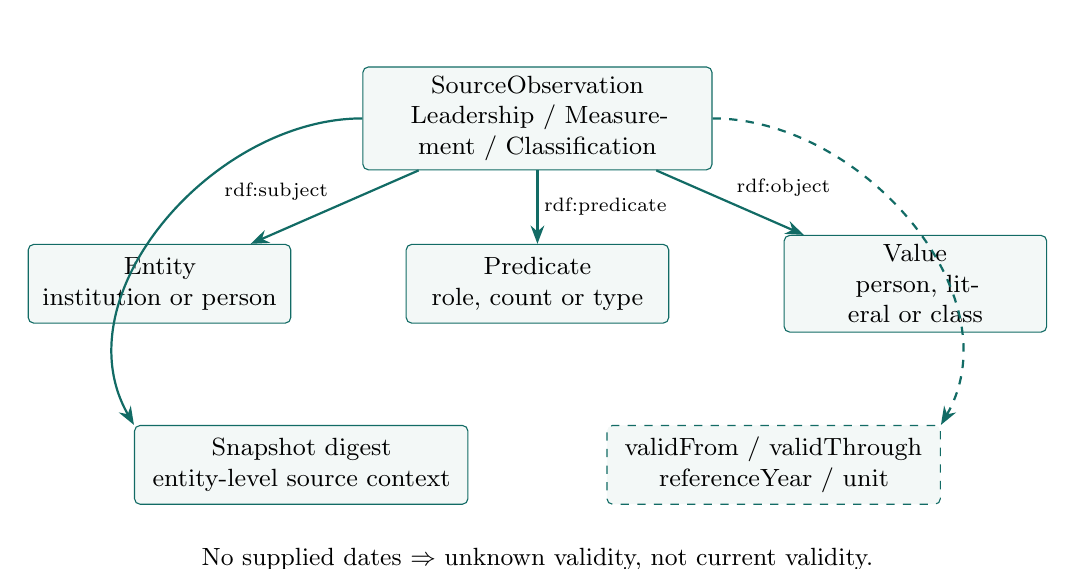
\begin{tikzpicture}
\node[auditbox,text width=4.2cm] (o) at (0,0) {SourceObservation\\Leadership / Measurement / Classification};
\node[auditbox,text width=3.1cm] (s) at (-4.8,-2.1) {Entity\\institution or person};
\node[auditbox,text width=3.1cm] (p) at (0,-2.1) {Predicate\\role, count or type};
\node[auditbox,text width=3.1cm] (v) at (4.8,-2.1) {Value\\person, literal or class};
\draw[auditarr] (o)--node[auditlabel,above left]{rdf:subject}(s);
\draw[auditarr] (o)--node[auditlabel,right]{rdf:predicate}(p);
\draw[auditarr] (o)--node[auditlabel,above right]{rdf:object}(v);
\node[auditbox,text width=4cm] (e) at (-3,-4.4) {Snapshot digest\\entity-level source context};
\node[auditbox,text width=4cm,dashed] (t) at (3,-4.4) {validFrom / validThrough\\referenceYear / unit};
\draw[auditarr] (o.west) to[out=180,in=120] (e.north west);
\draw[auditarr,dashed] (o.east) to[out=0,in=60] (t.north east);
\node[font=\small,align=center] at (0,-5.6) {No supplied dates $\Rightarrow$ unknown validity, not current validity.};
\end{tikzpicture}

\caption[Evidence-qualified temporal observations]{Observation model. Dashed fields are optional and must come
from evidence. Missing dates mean unknown temporal validity. The diagram is schematic;
no dates are fabricated for real officeholders.}\label{fig:observations}
\end{figure}

The implementation supports \term{validFrom}, \term{validThrough}, \term{referenceYear}
and measurement units, validates calendar dates and interval order, and retains normalized
SHA-256 digests of Silver inputs in \term{data/reports/observation-provenance.json}.
Copied source references provide \emph{entity-level context}, not proof that every assertion
occurs in every referenced source. The snapshot digest is not an upstream publication date.

The present Silver snapshot does not retain sufficient temporal qualifiers for these
measurements and appointments. Generated observations explicitly have unknown temporal
validity. The system does not infer today's leadership or a current enrollment total;
the institution infobox displays this limitation. Flat triples remain a source-snapshot
projection. Historical queries must require relevant date bounds on observations;
absence of an end date does not prove an appointment continues.

SHACL checks observation structure, allowed status, digest syntax, date datatypes and
interval ordering. Regression tests also verify that reification alone does not assert
the reified triple. This is a conservative migration, not a complete longitudinal
collection system. Acquiring actual dates, claim-level provenance, foundation events
and authoritative historical classifications remains future work.

\subsection{Competency questions and prohibited conclusions}
\begin{enumerate}
\item A direct body followed by its superior entails broad governance, not a second direct edge.
\item A council chair does not entail employment; an owner does not entail parenthood.
\item Joint providers or majors do not become identical through a program.
\item Recorded education does not entail the alumni class.
\item A current geographic crosswalk does not create a historical birthplace assertion.
\item An undated observation does not answer a date-valid question merely because it is in the latest export.
\end{enumerate}
Rule-engine execution, formal OWL profile membership, domain correctness and empirical
coverage remain distinct claims. The formal OWL 2 RL gate is now asserted only for the
committed release ontology, with its reproducible command and zero-violation evidence
recorded in \term{data/reports/owl2rl-profile.txt}.


\subsection{Materialization and temporal interpretation}
The system computes a rule closure over the local ontology and asserted data and retains
selected new instance-level statements. External identity links are joined into the
serving graph after this step. This avoids equality-driven copying to remote identifiers,
but means the published union is not a complete closure including all \term{owl:sameAs}
effects. The reported inferred-triple count describes the retained subset, not the full
internal closure.

Representative rules are:
\begin{align*}
\mathit{locatedIn}\circ\mathit{partOf}&\sqsubseteq\mathit{locatedIn},\\
\mathit{locatedIn}\circ\mathit{mergedInto}&\sqsubseteq\mathit{locatedIn},\\
\mathit{governedBy}\circ\mathit{subordinateTo}&\sqsubseteq\mathit{governedBy},\\
\mathit{offersProgram}\circ\mathit{ofMajor}&\sqsubseteq\mathit{trainsMajor}.
\end{align*}
For example, an institution assigned to a former province can also be related to the
successor province and its larger region. Inverse properties expose the same relationship
in the opposite direction without manually storing both directions in the asserted graph.

The model uses the \term{owlrl} implementation of OWL 2 RL/RDF rules. A separate OWL API
\term{OWL2RLProfile} gate checks the committed Turtle ontology; release 2.2 produced zero
violations. Calendar years are represented as \term{xsd:integer}, and calendar dates as
\term{xsd:dateTime} at midnight when the source supplies date precision only. This certifies
profile membership, not factual correctness, completeness over imported vocabularies, or
production performance.

The main temporal limitations are:
The \term{birthAreaInCurrentCrosswalk} chains are geographic containment crosswalks, separated from \term{bornIn} in version 2.2. Relating a birthplace to
a province created in 2025 does not mean that province existed when the person was born.
Similarly, historical institutions should not automatically be counted as currently
operating just because their location can be mapped to a current province. Queries for
current institutions should explicitly consider dissolution evidence and its incompleteness.

Version 2.2 adds qualified observations for roles, measurements and classifications, but
the available source snapshot still lacks sufficient temporal qualifiers and historical geographic versions. Absence of an end date is not proof of a current
appointment. Birth-date collection currently loses source precision, and suppressing
January 1 dates is only a heuristic: it can suppress real birthdays and cannot establish
the precision of all other dates. These source-quality limitations remain documented
work, not conclusions resolved by successful reasoning.

\section{Linking and publication}
This stage turns the validated graph into a Linked Data artifact. It has three distinct
responsibilities: interlink local resources with external datasets, expose useful Web
representations, and provide a query/storage runtime. The responsibilities are deliberately
not collapsed into one product: the Python transformer creates RDF, the publisher creates
resource documents, Protégé inspects ontology axioms, GraphDB is useful for interactive
exploration, and Fuseki provides the tested Apache Jena SPARQL/TDB2 path.

\begin{table}[htbp]\centering\small
\caption{Technology roles in the VN-Edu publication architecture.}\label{tab:technology-roles}
\begin{tabularx}{\textwidth}{p{3.0cm}XX}\toprule
Component & Main role & What it does not prove \\\midrule
Python/RDFLib pipeline & Integrates records, assigns URIs, emits RDF, materializes selected entailments & Does not provide a persistent public endpoint by itself \\
Protégé and OWL API & Inspects ontology axioms and checks OWL 2 RL profile membership & Does not validate all ABox facts or measure production capacity \\
GraphDB Workbench & Interactive repository loading, visualization, and SPARQL exploration & A layout is not a formal ontology specification \\
Apache Jena Fuseki/TDB2 & HTTP SPARQL/Graph Store access and persistent acceptance path & Does not mint canonical IRIs or establish factual accuracy \\
Silk Framework & Candidate entity-linking experiment on a frozen sample & Candidate links are not automatically accepted as \term{owl:sameAs} \\
\bottomrule
\end{tabularx}
\end{table}

\subsection{External relations}
The link graph contains \metricLinkTriples{} triples. Wikidata, ROR, GeoNames, and
selected DBpedia links use \term{owl:sameAs}; subject mappings use
\term{skos:closeMatch}; Wikipedia article links use \term{foaf:isPrimaryTopicOf}.
The last of these relates an entity to a document and must not be counted as an identity
assertion. Repeated attempts to add the same link no longer inflate linkset counters.

Shared identifiers are useful identity evidence, but errors and historical scope
mismatches can occur in the source mappings. Some organizational links are discovered
through label matching with contextual filters. These deserve separate manual review.
The audit does not certify every identity link or every administrative boundary match.

\subsection{Representations and deployment}
The static publisher generates HTML pages, embedded JSON-LD, and RDF files. The dynamic
server provides query handling and RDF content negotiation. The canonical namespace
currently belongs to GitHub Pages; the dynamic service has another origin. Content
negotiation at the dynamic service does not establish that the canonical static URI
performs the same negotiation.

The implementation supports practices associated with five-star Linked Open Data.
Section~\ref{sec:five-star} assesses each level and reports a small, dated HTTP sample;
it does not reuse the earlier report's live availability measurements. The repository
declares project licensing, retains source-specific rights metadata, and does not purport
to relicense upstream material. In particular, the Ministry admissions source does not
state a machine-readable open-data licence; its official facts are attributed and their
reuse remains subject to the source's terms. This audit is not legal advice or a legal
verification of every upstream asset.

The publisher now checks its output path before recursive replacement. It refuses the
project root, external paths, symbolic links, and existing directories without generated-site
markers. This prevents a misconfigured output environment variable from deleting source
data or the project itself.

\subsection{User-facing resource and query views}
The publication layer is also evaluated from the perspective of a reader and a
developer. Figure~\ref{fig:resource-page} shows a generated resource page for a
university. It exposes the canonical IRI, labels, source context, external links,
and machine-readable affordances without requiring a user to inspect the raw Turtle
file. Figure~\ref{fig:sparql-ui} shows the separate SPARQL interface used to submit
read-only competency queries and inspect tabular results. These screenshots document
the user interface only; endpoint availability, persistence, graph parity, and the
read-only policy are established by the automated acceptance tests described in
Section~\ref{sec:fuseki}.

\begin{figure}[htbp]
\centering
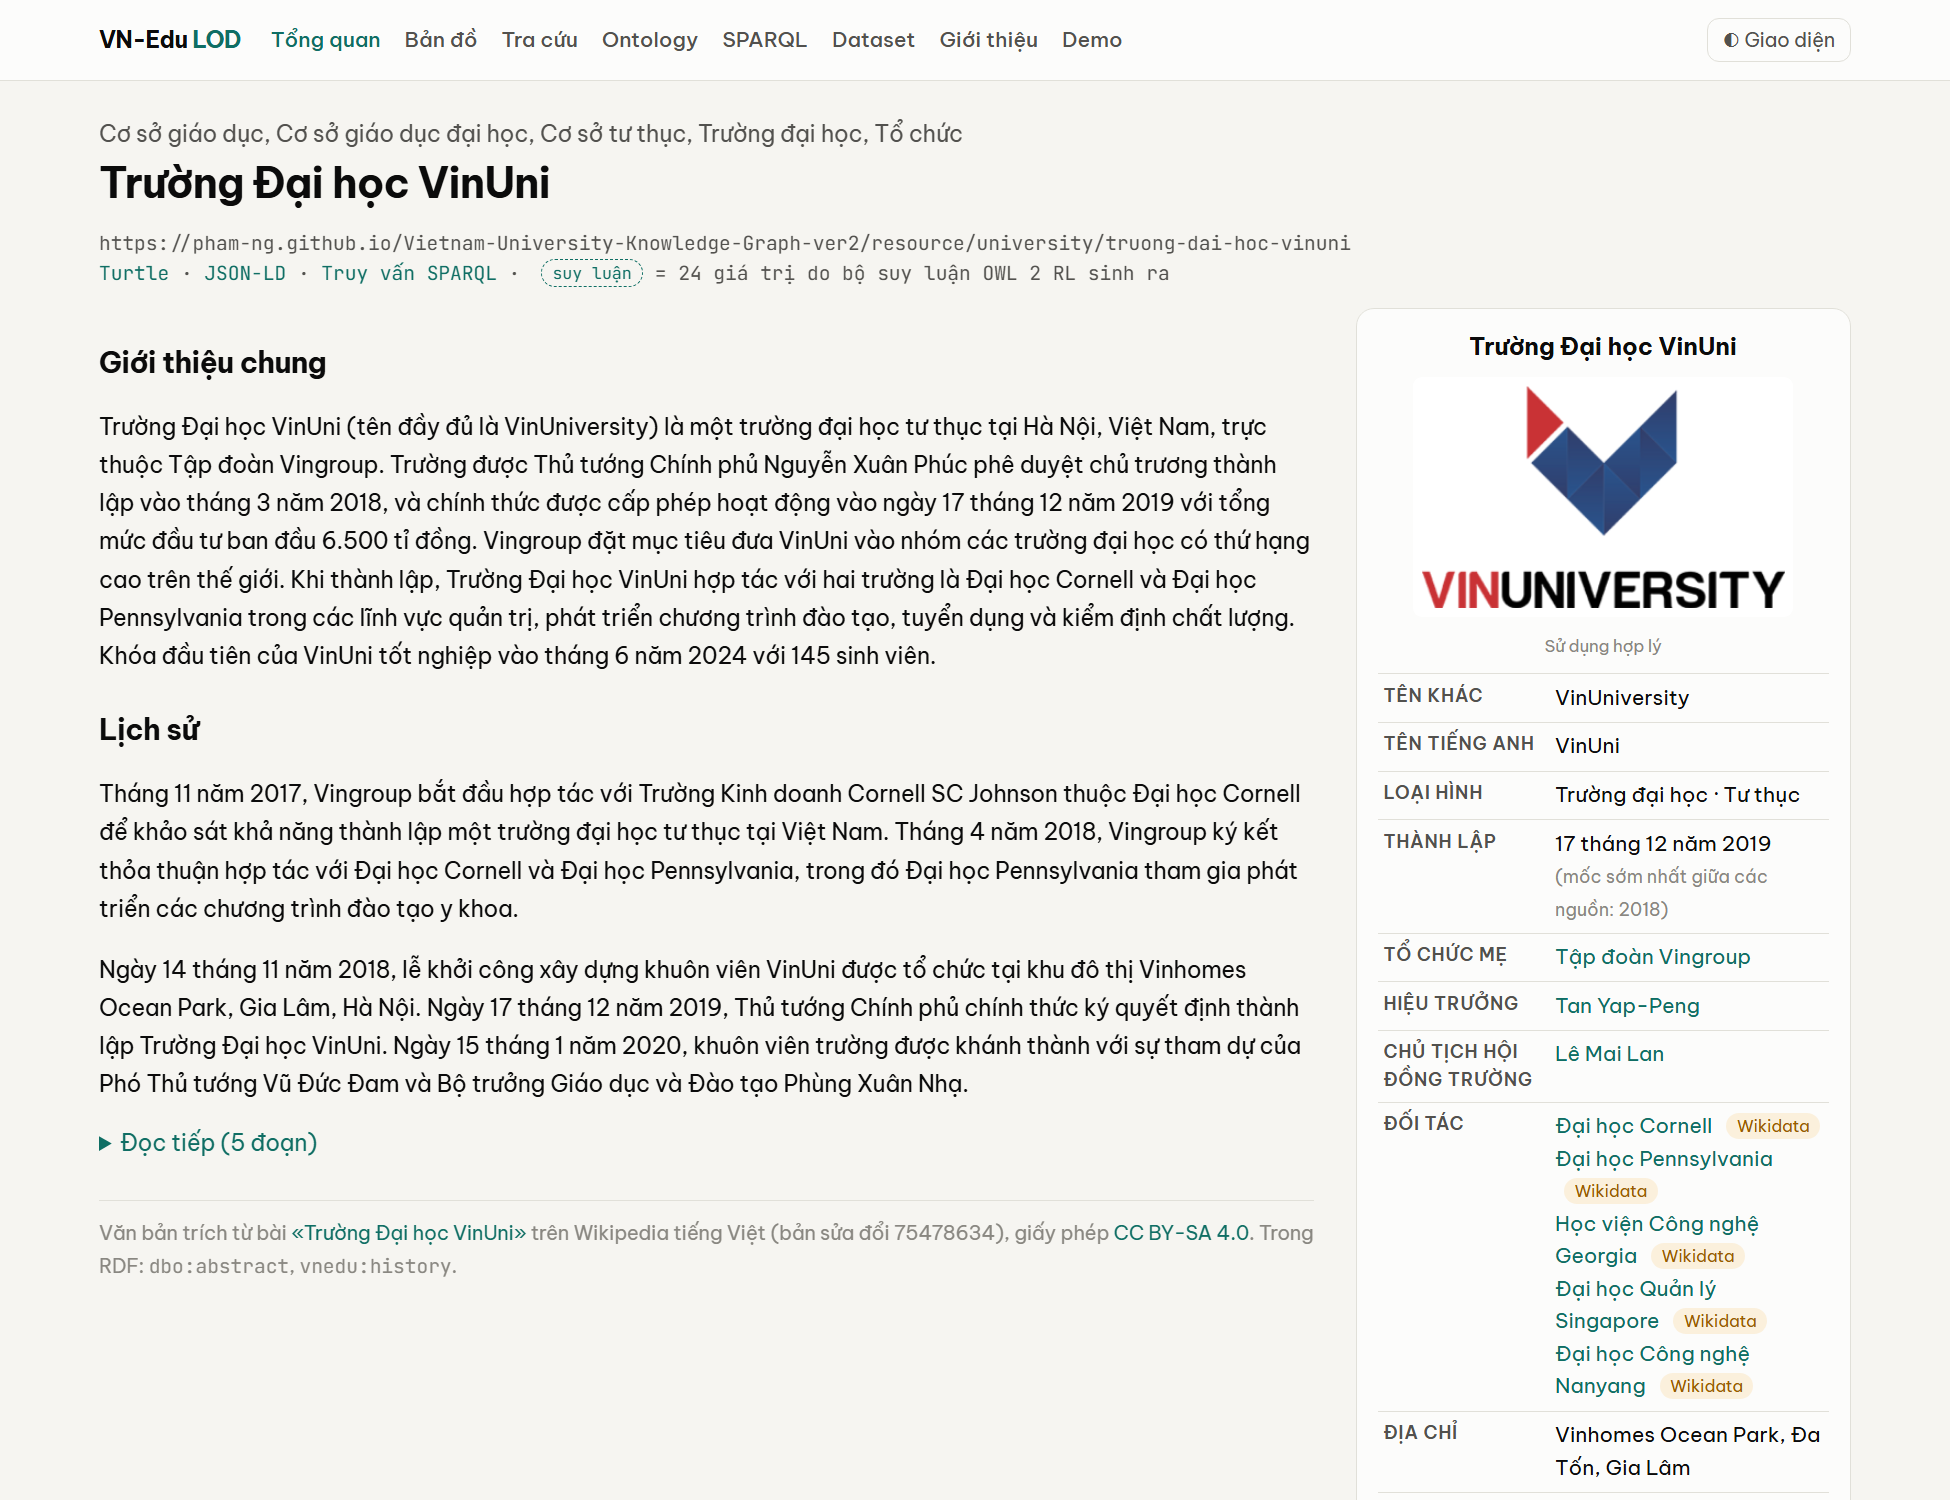
\includegraphics[width=0.94\textwidth]{figures/resource.png}
\caption{Generated Linked Data resource view for a university.}
\label{fig:resource-page}
\end{figure}

\begin{figure}[htbp]
\centering
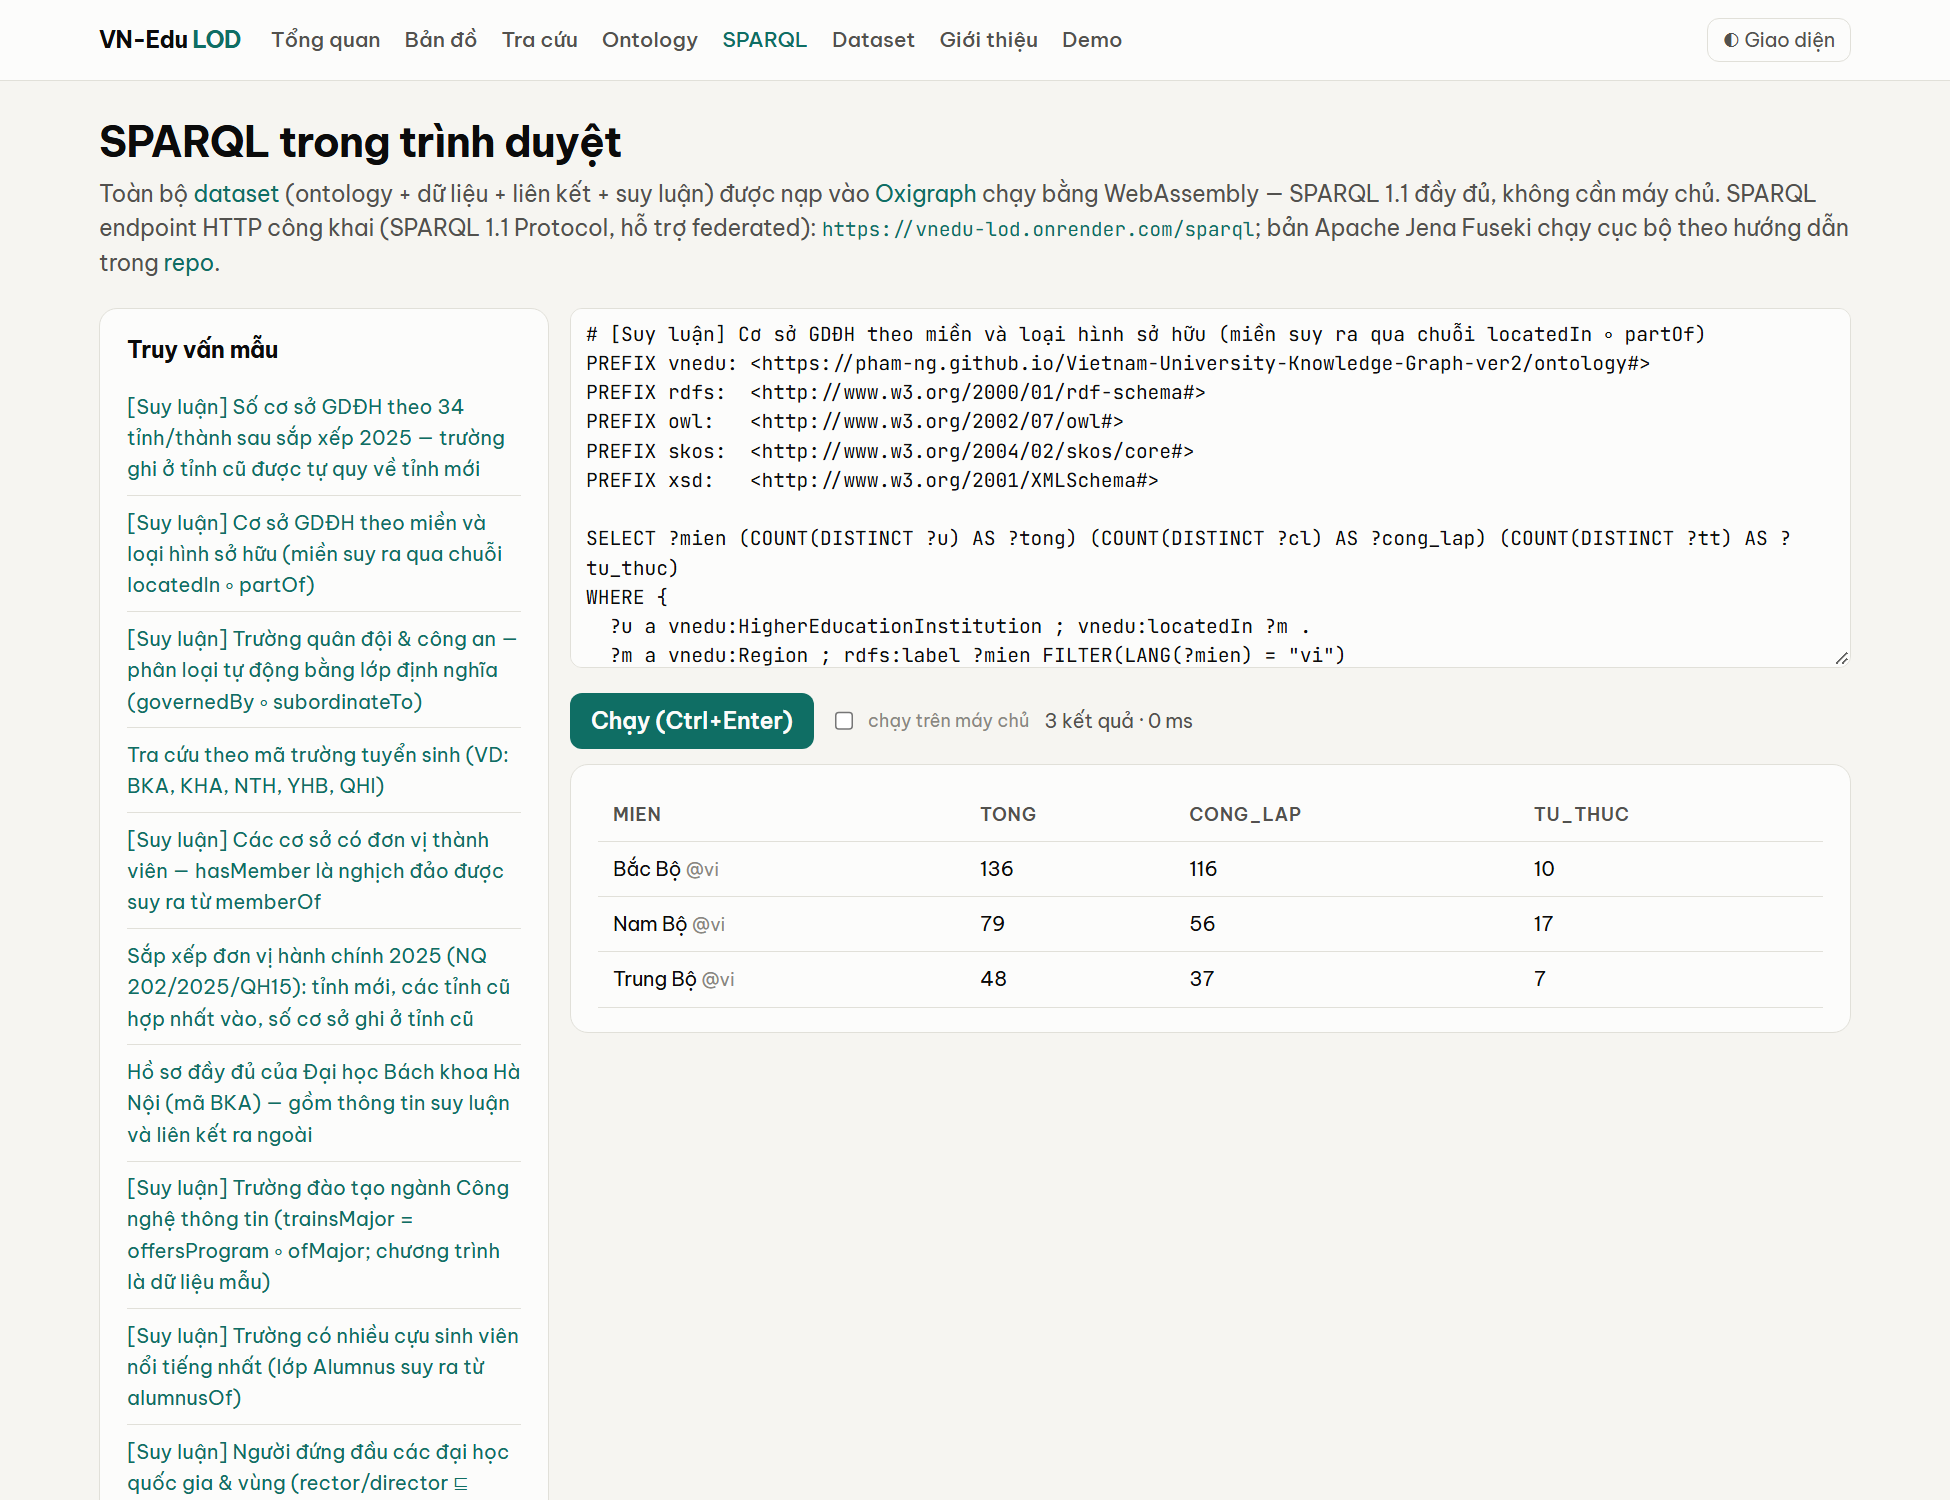
\includegraphics[width=0.94\textwidth]{figures/sparql.png}
\caption{Read-only SPARQL query view and returned result table.}
\label{fig:sparql-ui}
\end{figure}

\section{Deployment and Apache Jena Fuseki}
\label{sec:fuseki}
This section documents how the validated RDF release is published and queried. It is useful
to separate the URI design from the runtime: a URI identifies a resource, while Fuseki stores
and queries triples about that resource. The same graph can therefore be published as static
RDF and loaded into Fuseki without changing its identifiers.
Fuseki is a SPARQL server, not a URI minting service~\cite{fuseki}.
The transformer assigns canonical identifiers before data enters any store.
The same university IRI remains in RDF whether queried by RDFLib, Oxigraph or Fuseki.

\Needspace{15\baselineskip}
\subsection{Identity, representation and storage}
\begin{code}
# RDF subject identifying a university:
https://pham-ng.github.io/Vietnam-University-Knowledge-Graph-ver2/resource/university/dai-hoc-bach-khoa-ha-noi
# Local query endpoint:
http://localhost:3030/vnedu/sparql
# Graph Store Protocol target:
http://localhost:3030/vnedu/data?default
\end{code}
Uploading RDF does not make its canonical IRIs dereferenceable automatically.
The publisher independently creates HTML, Turtle and JSON-LD descriptions. Ontology terms
retain hash IRIs; entity and observation identifiers use slash paths.
Immutable 2.1 and 2.2 version artifacts are generated under \term{ontology/}.
Dynamic version routes support RDF content negotiation and return 404 for unknown versions.

GitHub Pages remains a separate HTTP origin from Flask. Its static representation links
and embedded JSON-LD do not implement Flask's negotiation, nor the entity-to-document
303 pattern discussed in \emph{Cool URIs}~\cite{uris}. Adding Fuseki cannot fix those origin-level
behaviors. Version artifacts are implemented and tested in the release; availability from
each public origin remains an HTTP-deployment concern rather than an ontology property.

\begin{figure}[htbp]\centering
\resizebox{\textwidth}{!}{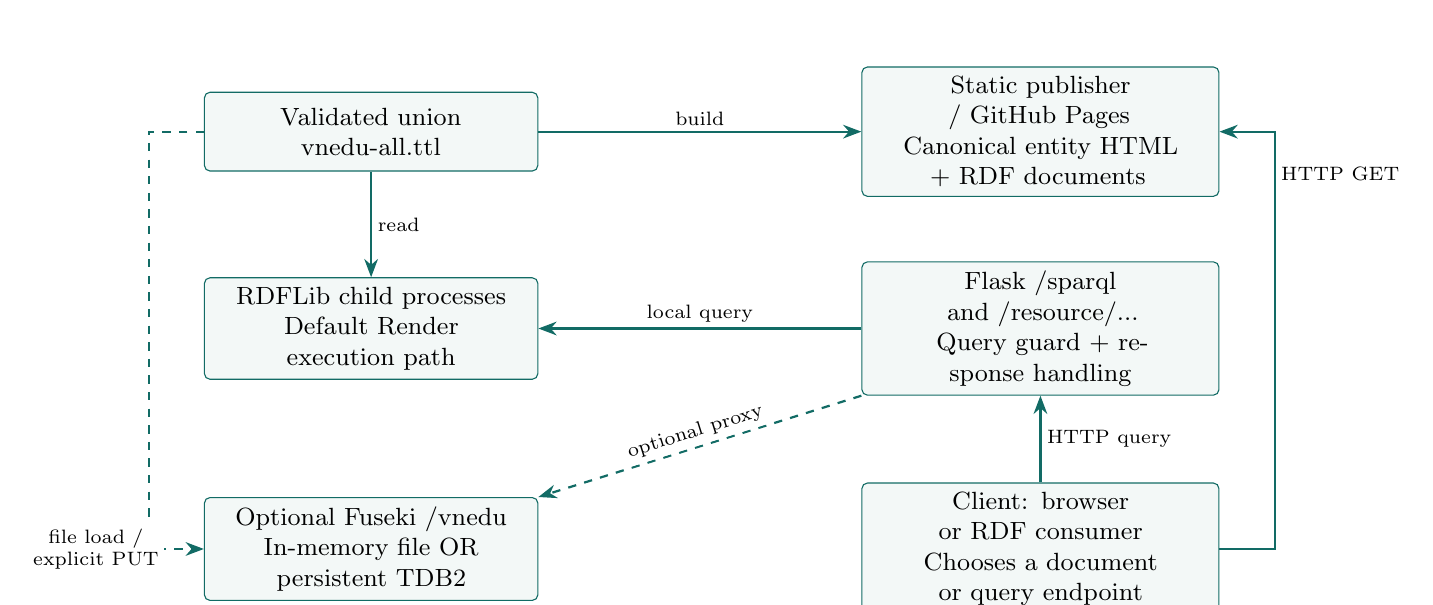
\begin{tikzpicture}
\node[auditbox,text width=4cm] (gold) at (0,0) {Validated union\\vnedu-all.ttl};
\node[auditbox,text width=4.3cm] (static) at (8.5,0) {Static publisher / GitHub Pages\\Canonical entity HTML + RDF documents};
\node[auditbox,text width=4cm] (rdf) at (0,-2.5) {RDFLib child processes\\Default Render execution path};
\node[auditbox,text width=4.3cm] (flask) at (8.5,-2.5) {Flask /sparql and /resource/...\\Query guard + response handling};
\node[auditbox,text width=4cm] (fuseki) at (0,-5.3) {Optional Fuseki /vnedu\\In-memory file OR persistent TDB2};
\node[auditbox,text width=4.3cm] (client) at (8.5,-5.3) {Client: browser or RDF consumer\\Chooses a document or query endpoint};
\draw[auditarr] (gold)--node[auditlabel,above]{build}(static);
\draw[auditarr] (gold)--node[auditlabel,right]{read}(rdf);
\draw[auditarr] (flask)--node[auditlabel,above]{local query}(rdf);
\draw[auditarr,dashed] (gold.west) -- ++(-0.7,0) |- node[auditlabel,pos=0.65,left]{file load /\\explicit PUT}(fuseki.west);
\draw[auditarr,dashed] (flask.south west)--node[auditlabel,sloped,above]{optional proxy}(fuseki.north east);
\draw[auditarr] (client)--node[auditlabel,right]{HTTP query}(flask);
\draw[auditarr] (client.east)--++(0.7,0)|-node[auditlabel,pos=0.45,right]{HTTP GET}(static.east);
\end{tikzpicture}
}
\caption[URI publication and optional Fuseki execution]{Publication and storage paths. The optional Fuseki
branch has verified Linux and Windows acceptance runs; Render still explicitly selects local RDFLib.
Storage does not replace the canonical identifiers.}\label{fig:deployment}
\end{figure}

\subsection{Safe loading and reproducible runtime}
The revised loader requires a successfully validated release before network writes.
It targets an existing explicitly named dataset rather than creating one implicitly.
An empty graph can be loaded directly. Replacement of a nonempty default graph requires
both \term{--replace} and a new \term{--backup} path; the backup is created exclusively,
so an older backup cannot be silently overwritten. HTTP redirects and error responses are
rejected. After PUT, the loader retrieves the entire default graph and checks RDF graph
isomorphism, including blank nodes, rather than relying on a triple count.

Graph Store PUT replaces the selected graph~\cite{gsp}; named graphs are untouched by
this loader. Credentials are read from environment variables, not command-line passwords.
A failed comparison preserves the backup for operator recovery; it is not a distributed
transaction or automatic rollback. Operators must stop concurrent writers during a release:
a backup followed by PUT does not provide compare-and-swap concurrency control.

The runtime setup pins Apache Jena Fuseki 6.2.0 and verifies its published SHA-512 digest.
The local launcher requires Java 21, validates the release, binds to loopback, and enables
only query access with a configured timeout. Its file mode reloads the graph at startup;
the separate acceptance harness explicitly tests persistent TDB2.
The optional legacy Docker recipe now requires an operator-selected image and password,
and binds port 3030 only on loopback. That Docker configuration was not the tested runtime.

\subsection{Production-like security and performance acceptance}
The additional \term{audit/production\_readiness.py} test starts the same Waitress WSGI
entry point used by \term{app/server.py --prod} with the read-only local backend. Under
normal bounded concurrency, all eight constant-time health requests returned HTTP 200; the
final 9 October 2026 rerun measured 12.45 ms at p50, 15.89 ms at p95 and 15.89 ms maximum
on the Windows review machine. An intentional simultaneous eight-request SPARQL overload
against two query workers returned two HTTP 200 responses and six HTTP 503 responses,
demonstrating bounded back-pressure rather than unbounded query growth. A parser lock also
prevents concurrent cold requests from racing RDFLib's lazy SPARQL grammar initialization.
Security probes rejected a path-injection
attempt (404), an unapproved SSRF \term{SERVICE} target (400), and an oversized query (413).
The response headers now include \term{nosniff}, \term{SAMEORIGIN}, strict referrer-policy,
\term{Permissions-Policy}, CSP on HTML, and an \term{X-Request-ID}; HSTS is enabled when
TLS is detected or explicitly forced behind a trusted TLS terminator.

These numbers are a reproducible loopback acceptance sample, not a capacity SLO, penetration
test, TLS/reverse-proxy audit, cloud IAM review, or production security certification. The
bounded persistent RDFLib worker deliberately trades throughput for isolation; a real
deployment still needs external rate limiting, resource quotas, TLS termination, monitoring,
authentication policy, and a load test against its selected Fuseki/WSGI topology. The full
machine-readable evidence is \term{data/reports/production-readiness.json}.

\subsection{Production hardening profile and release gates}
The review branch adds a deployable reference profile in \term{deploy/} and records its
scope in \term{docs/production-readiness.md}. The intended production path is:
\begin{code}
Internet -> Caddy/Nginx TLS -> Waitress application -> private Fuseki -> encrypted TDB2 volume
\end{code}
The application layer is read-only for SPARQL, limits request bodies and serialized result
size, applies an optional per-client rate limit, restricts CORS to an explicit allow-list,
and emits request identifiers for incident correlation. The reference Compose file also
uses a non-root application user, a read-only container filesystem, a private network,
dropped Linux capabilities and a no-new-privileges flag. Fuseki image digests and admin
credentials are deliberately operator-supplied; the public reverse proxy must never expose
Fuseki administration or update endpoints.

Some application-layer controls are active on the public Render service, but this is not
evidence that the complete reverse-proxy/Fuseki/TDB2 profile has been deployed. Before a
production claim for that topology, the deployed Fuseki path
must be tested for sustained and burst requests, p50/p95/p99 latency, CPU/memory/disk
growth, query cancellation, rolling restart and backup restoration. The current local
RDFLib p95 is therefore reported as an isolation/back-pressure observation, not as a
capacity target.

\begin{table}[htbp]\centering\small
\caption{Production release gates that remain separate from OWL and SHACL conformance.}
\label{tab:production-gates}
\begin{tabularx}{\textwidth}{p{4.2cm}X}\toprule
Gate & Required evidence before an authoritative production claim \\\midrule
Security deployment & Public TLS termination, trusted proxy configuration, firewall/IAM policy, secret rotation and external rate limits. \\
High-load performance & Deployed Fuseki benchmark with representative SELECT/CONSTRUCT queries, p50/p95/p99, saturation behavior and resource measurements. \\
Recovery & The immutable publication ZIP was restored and hash/parse checked locally; runtime database snapshots, off-host retention and rolling restore remain operator gates. \\
Factual accuracy & Independent adjudication of the five founding-year conflicts and seven unresolved values, plus a held-out identity-link evaluation. \\
Temporal validity & Claim-level provenance and validity intervals for leadership, enrolment and legal status; undated snapshots must not be presented as current. \\
Source authority & Official-register or institution-owner evidence for records currently supported only by encyclopedic or inferred sources. \\
\bottomrule\end{tabularx}
\end{table}

The release can pass the OWL 2 RL profile gate, SHACL validation and regression tests while
still failing these operational and factual gates. Keeping those gates separate is essential:
OWL entailment is not a truth certificate, and a five-star Linked Data publication is not a
five-star security or accuracy certification.

\subsection{Executed end-to-end acceptance evidence}
The primary reproducible test ran on Linux GitHub Actions with Fuseki 6.2.0 and Temurin Java 21.0.12.1,
on 7 October 2026 at 01:50 UTC. The latest Windows run began on 9 October 2026 at
03:50:45 UTC and used the same pinned Fuseki JAR, Java 21.0.8 and the selector/socket
workaround against the current 87,183-triple release. An accidental invocation through the
Java 8 executable failed before startup because Fuseki 6.2 requires class-file version 65;
rerunning with the explicitly selected JDK 21 completed successfully. This is useful runtime
selection evidence rather than a semantic or data failure.
The input hash, JAR hash, runtime details and assertions are archived in
\term{data/reports/fuseki-e2e-linux.json} and the Windows run in
\term{data/reports/fuseki-e2e-windows.json}; the corresponding Linux
\href{https://github.com/pham-ng/Vietnam-University-Knowledge-Graph-ver2/actions/runs/37559070543}{CI run}
completed successfully.

\begin{table}[htbp]\centering\small
\caption{Measured Fuseki/TDB2 acceptance results.}\label{tab:fuseki-status}
\begin{tabularx}{\textwidth}{P{6.5cm}X}\toprule
Check & Observed result \\\midrule
Load complete validated serving graph & 87,183 triples; graph-isomorphic to local RDF. \\
Attempt unapproved replacement & Refused before PUT. \\
Approved replacement with backup & Backup graph-isomorphic to previous contents. \\
Query parity with RDFLib & Count: 1 row; class totals: 68 rows; programs: 78 rows; explicitly dated leadership: 0 rows. \\
Stop and restart with the same TDB2 directory & Entire default graph remains isomorphic. \\
Restart without update permission & SPARQL Update and Graph Store PUT both return HTTP 405. \\
Read after rejected writes & Graph unchanged and isomorphic. \\
\bottomrule\end{tabularx}
\end{table}

The test uses a newly created disposable directory and ephemeral loopback port; no existing
user dataset is overwritten. Zero dated-leadership rows is an honest reflection of missing
date evidence, not a failed lookup to be filled with invented dates.

On Windows, the first attempt exposed a JDK 21 selector/socket initialization failure.
The repaired launcher now sets the selector provider and short Unix-domain socket directory
through inherited Java options (avoiding PowerShell 5.1 argument concatenation); the same
disposable TDB2 acceptance test then passed all checks, and a direct query-only launcher
smoke test returned HTTP 200. This proves local Windows operability, not production deployment.
Configured timeout is not proof of cancellation under load. Authentication, SERVICE egress,
concurrent writers, memory limits, disaster recovery and production TLS require separate
acceptance tests. The verified read-only mode is access restriction, not a full security certification.

\section{Five-star Linked Open Data assessment}
\label{sec:five-star}
The five-star scheme evaluates how data is published and connected, not the overall
quality of a program or the correctness of every ontology axiom~\cite{five}. There is no
Fuseki-specific requirement: RDFLib or static RDF publication can support the relevant
mechanisms. Table~\ref{tab:five-stars} assesses the project's data publication rather than
assigning an unsupported software-quality score.

\begin{table}[htbp]\centering\small
\caption{Evidence against the cumulative five-star publication scheme.}\label{tab:five-stars}
\begin{tabularx}{\textwidth}{p{1cm}p{3.8cm}X}\toprule
Level & Criterion, summarized & Project evidence and qualification \\\midrule
1 & Publicly accessible, with reuse terms & Public sample accessible; CC BY-SA 4.0 covers project-controlled compilation and material. Upstream rights remain source-specific; the Ministry source has no stated machine-readable open-data licence. \\
2 & Structured, machine-readable & JSON records and parsed RDF graphs, not only screen images or PDFs. \\
3 & Non-proprietary format & JSON, Turtle and JSON-LD artifacts. \\
4 & Web identifiers and open Semantic Web standards & Stable-registry HTTP IRIs, RDF descriptions and query interfaces; sampled entity documents parse. Canonical negotiation remains static; version artifacts are now implemented on the review branch. \\
5 & Connections to other datasets & Corrected local link graph contains 2,309 \term{owl:sameAs}, 61 \term{skos:closeMatch} and 1,188 document-topic links. Existence is measured; every identity assertion is not independently verified. \\
\bottomrule\end{tabularx}
\end{table}

\textbf{Verdict.} The implementation and sampled public RDF support the five-star
publication pattern, subject to the declared licensing scope. Commit \term{a977a239} was
observed live on Render on 9 October 2026 with the corrected 87,183-triple release. This is
not an independent certification, proof of every fact, or proof of a production-grade SLA.
Temporal-evidence and operations limits must therefore accompany the claim rather than be
hidden by a five-star badge.

\subsection{Dated HTTP evidence}
The public Render deployment was checked after manual promotion of commit
\term{a977a239} on 9 October 2026. The checks used bounded read-only HTTP requests against
\url{https://vnedu-lod.onrender.com}; this is an acceptance sample, not continuous
monitoring or a random workload.

\begin{table}[htbp]\centering\small
\caption{Observed HTTP behavior of the deployed corrected release.}\label{tab:http-check}
\begin{tabularx}{\textwidth}{p{4.5cm}X}\toprule
Request & Observation \\\midrule
Render \term{/healthz} & HTTP 200; status \term{ok}, backend \term{rdflib (persistent isolated worker)}, commit \term{a977a239}. \\
Three full triple-count queries & All returned 87,183; observed response times were 11,313, 8,742 and 8,421 ms. \\
Institutional-membership query & Four distinct HUS/HCMUS/USSH results had the intended Hanoi or Ho Chi Minh City parent and an inferred inverse \term{hasMember}; HTTP 200 in 3,477 ms. \\
HUST entity, Accept Turtle & HTTP 200, \term{text/turtle}, 13,347 bytes, 2,653 ms. \\
SPARQL Update attempt & HTTP 400; public query surface remained read-only. \\
Unapproved federated \term{SERVICE} target & HTTP 400; the SSRF allow-list rejected the target. \\
Latest local Fuseki/TDB2 E2E & 87,183 triples loaded, queried, restarted and graph-isomorphism checked; writes rejected with HTTP 405. \\
\bottomrule\end{tabularx}
\end{table}

The Render deployment took 5 minutes 27 seconds and generated the static site during startup;
this is operationally inefficient. The free service can cold-start, uses one bounded query
worker, and the measured 8--11 second full counts are not a high-load benchmark or SLO.
The public runtime uses RDFLib, not the separately accepted Fuseki/TDB2 topology. The probes
do not establish sustained capacity, admin security, backup recovery, or external penetration
test results. They do establish sampled public availability, deployed-revision identity,
read-only behavior and query correctness for the stated release.

The media distinction also matters. For example, the shipped HUST logo metadata records
``fair use'' while its campus photograph records CC0. Describing or linking such an image
does not relicense the image under the dataset license. The revised publisher shows a source link, not an embedded image, for unknown, fair-use or unrecognized licenses. A data publication claim must not
be expanded into a blanket claim that every remotely displayed asset is openly licensed.


\section{Application security and query execution}
The original SPARQL policy searched for textual patterns containing whitespace after
\term{SERVICE} and \term{FROM}. Valid forms without that whitespace bypassed the filter.
The audit reproduced this locally using loopback targets without issuing an outbound
request. The revised policy inspects parsed SPARQL operations and permits only two exact
HTTPS service endpoints. It rejects dataset-loading clauses, variable service targets,
alternate ports, credentials, and arbitrary paths. Security keywords inside string
literals are not treated as operations. The local outbound HTTP handler also rejects
redirects.

The previous timeout waited only for \term{Graph.query} to return. RDFLib can evaluate
SELECT bindings lazily, so result evaluation could continue beyond the limit.
Cancelling a future also cannot stop an already running Python thread. The revised local
backend evaluates and serializes each query in a disposable process, terminates it on
timeout, and limits concurrent workers. An expensive Cartesian-product regression test
checks that capacity is released and a subsequent small query succeeds.

The local backend limits serialized responses to 8 MiB. This does not impose a hard
memory limit during intermediate evaluation, and parsing the public request still occurs
in the web process. A hostile-workload production deployment therefore needs process or
container memory limits, request-rate controls, and appropriate upstream isolation. The
process-per-query approach also reloads the graph and has a throughput cost. Earlier
in-memory latency measurements do not describe this implementation.

The Fuseki proxy supplies an execution timeout parameter and does not follow proxy
redirects. Actual query cancellation and remote SERVICE egress remain responsibilities
of the configured Fuseki instance. The separate Linux acceptance run verifies load/query/persistence/read-only behavior;
it does not verify production federation controls. Raw POST requests with \term{application/sparql-query} are now accepted,
alongside form-encoded query requests.

The security tests support a bounded local read-only service: path traversal, unapproved
federation targets, oversized queries, and uncontrolled worker growth are rejected by the
implemented checks. These are application-level controls. They do not replace TLS termination,
authentication, external rate limiting, memory quotas, secret rotation, monitoring, or a
deployed Fuseki load test. The production topology and its remaining gates are documented in
Section~\ref{sec:fuseki}.

\section{Reproducible workflow and CI/CD}
\label{sec:cicd}
The repository uses continuous integration as a reproducibility mechanism, not as a substitute
for scientific interpretation. Figure~\ref{fig:cicd-workflow} shows the ordinary release path
and the two specialized evidence paths. The main workflow rebuilds the graph and static site,
while Fuseki and Silk run in separate workflows with their own runtime requirements.

\begin{figure}[htbp]\centering
\resizebox{\textwidth}{!}{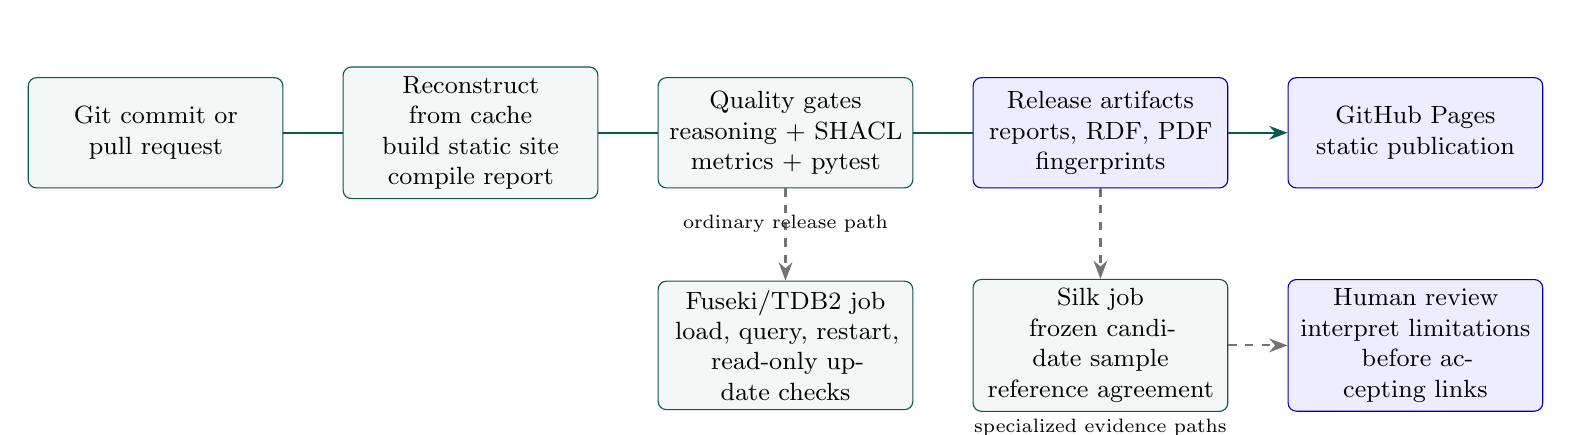
\begin{tikzpicture}[
  node distance=8mm and 7mm,
  job/.style={draw=accent!80!black, rounded corners=3pt, fill=accent!5, align=center, font=\small, text width=3.0cm, minimum height=14mm},
  evidence/.style={draw=blue!70!black, rounded corners=3pt, fill=blue!7, align=center, font=\small, text width=3.0cm, minimum height=14mm},
  arr/.style={-{Stealth}, thick, draw=accent!80!black},
  branch/.style={-{Stealth}, dashed, thick, draw=black!55}
]
\node[job] (commit) at (0,0) {Git commit or pull request};
\node[job] (build) at (4.0,0) {Reconstruct from cache\\build static site\\compile report};
\node[job] (gates) at (8.0,0) {Quality gates\\reasoning + SHACL\\metrics + pytest};
\node[evidence] (artifact) at (12.0,0) {Release artifacts\\reports, RDF, PDF\\fingerprints};
\node[evidence] (pages) at (16.0,0) {GitHub Pages\\static publication};

\node[job] (fuseki) at (8.0,-2.7) {Fuseki/TDB2 job\\load, query, restart,\\read-only update checks};
\node[job] (silk) at (12.0,-2.7) {Silk job\\frozen candidate sample\\reference agreement};
\node[evidence] (review) at (16.0,-2.7) {Human review\\interpret limitations\\before accepting links};

\draw[arr] (commit)--(build)--(gates)--(artifact)--(pages);
\draw[branch] (gates)--(fuseki);
\draw[branch] (artifact)--(silk);
\draw[branch] (silk)--(review);
\node[font=\scriptsize, align=center] at (8,-1.15) {ordinary release path};
\node[font=\scriptsize, align=center] at (12,-3.75) {specialized evidence paths};
\end{tikzpicture}
}
\caption[CI/CD and evidence workflow]{CI/CD workflow. A commit enters the ordinary reconstruction
and quality gates; successful artifacts can be published to GitHub Pages. Fuseki/TDB2 and Silk
are separate evidence paths with different acceptance claims.}
\label{fig:cicd-workflow}
\end{figure}

\subsection{Release sequence}
The release sequence is intentionally ordered. Inputs are reconstructed first, RDF is then
materialized and checked, and only a release with matching fingerprints can be published or
loaded into Fuseki. A failure in a later gate does not turn a candidate graph into a public
graph. This design addresses a common failure mode in data projects: reporting a successful
transformation before validating the exact artifact that is served.

\begin{enumerate}
\item Reconstruct cached inputs and validate Silver records.
\item Generate asserted RDF, link metadata, ontology data, and selected inferred triples.
\item Run OWL diagnostics, SHACL, metrics, stale-release checks, and graph-isomorphism checks.
\item Build the static publication and the report from the accepted artifact.
\item Run the Fuseki/TDB2 acceptance job and, when requested, the isolated Silk experiment.
\end{enumerate}

\subsection{What CI proves}
The current suite demonstrates reproducible execution of the declared local gates. It does
not prove that every institution is represented, every identity link is correct, or that the
public endpoint can sustain an arbitrary workload. Those claims require independent annotation,
authoritative source comparison, and a load test against the selected production topology.


\section{Evaluation and results}
\subsection{Release measurements}
All values in Table~\ref{tab:size} are generated by \term{audit/release\_metrics.py} from
the validated local release. That script also checks that the serving graph is isomorphic
to the union of its declared components. It does not request data from a remote endpoint.
\begin{table}[htbp]\centering
\caption{Measured size of the corrected local release.}\label{tab:size}
\begin{tabularx}{\textwidth}{Xr}\toprule
Quantity & Count \\\midrule
Educational-organization records & \metricInstitutions{} \\
Classified higher-education institutions & \metricHEIs{} \\
Person records & \metricPeople{} \\
Institution-leader records & \metricLeaders{} \\
People with recorded education relations & \metricEducationParticipants{} \\
Current / former province-level units & \metricCurrentProvinces{} / \metricFormerProvinces{} \\
Illustrative programs / majors & \metricPrograms{} / \metricMajors{} \\
Asserted data triples & \metricAssertedTriples{} \\
Retained inferred triples & \metricInferredTriples{} \\
Link-graph triples & \metricLinkTriples{} \\
Ontology / dataset-metadata triples & \metricOntologyTriples{} / \metricMetadataTriples{} \\
Distinct triples in serving union & \metricUnionTriples{} \\
Local resource IRIs appearing as subjects & \metricLocalResources{} \\
\bottomrule\end{tabularx}
\end{table}

In the corrected snapshot, selected SHACL checks report \metricViolations{} violations,
\metricWarnings{} warnings, and \metricInformationResults{} informational result.
Warnings include missing foundation years and institution locations. Warning-tolerant
conformance means the configured release policy permits these omissions; it does not
mean all records are complete. The consistency diagnostics report no detected local
violations after the fixes.

Field coverage uses all 300 institution records as its denominator: 278 have a selected
foundation year, 288 a province reference, 256 an ownership value, 237 a website, 175
coordinates, 60 an admission code, and 28 a student-count value. These are presence
measurements, not estimates of truth, timeliness, or national coverage. In particular,
271 higher-education classifications and 300 educational-organization records are
different denominators and should not be interchanged.

\subsection{Link experiment: agreement, not independent accuracy}
The available experiment uses 86 institutions with English labels and identifier-derived
DBpedia reference targets. A local token-Jaccard matcher selects the highest-scoring target
from that closed reference candidate set. Table~\ref{tab:agreement} reports agreement with
the reference frozen from revision \term{58c65f0}. This baseline is not Silk;
the separate actual Silk execution is reported below.
\begin{table}[htbp]\centering\small
\caption{Token-Jaccard agreement with the identifier-derived reference.}\label{tab:agreement}
\begin{tabular}{rrrrrr}\toprule
Threshold & Predictions & Disagreements & Ref. precision & Ref. recall & Ref. F1 \\\midrule
0.2 & 85 & 13 & 84.7\% & 83.7\% & 0.842 \\
0.4 & 80 & 8 & 90.0\% & 83.7\% & 0.867 \\
0.6 & 76 & 6 & 92.1\% & 81.4\% & 0.864 \\
0.8 & 68 & 4 & 94.1\% & 74.4\% & 0.831 \\
1.0 & 58 & 1 & 98.3\% & 66.3\% & 0.792 \\
\bottomrule\end{tabular}
\end{table}

Let $M$ be the set of predictions, $R$ the reference pairs, and $TP=|M\cap R|$.
The reported precision is $TP/|M|$, recall is $TP/|R|$, and F1 is their harmonic mean.
Calling $R$ independent ground truth would be incorrect because the identifier linker
generated it. Scoring that same linker against $R$ yields perfect agreement by construction.
The previous claim of 100\% linking accuracy is therefore withdrawn.

The selected sample excludes unlinked institutions and targets outside the reference set.
These restrictions affect task difficulty and coverage. The threshold with the highest F1
on this sample is a descriptive observation, not a validated threshold chosen on a separate
development set. A defensible accuracy study needs independently annotated links and
non-links, dated evidence, an adjudication procedure, and a held-out test set.

\subsection{Executed Silk Framework experiment}
A separate experiment now executes actual Silk Framework 3.6.0, rather than referring
to the Python Jaccard baseline as Silk. The official single-machine entry point was
compiled with Scala 2.12.10 against released workbench libraries and run on Java 8.
Pinned checksums are in \term{audit/setup\_runtimes.ps1}; the runner, XML rules, input
N-Triples, candidate outputs and result JSON are included in the repository.

The experiment freezes the 86-source/86-target sample from revision \term{58c65f0},
giving 7,396 possible pairs. Both methods use the same lowercased English labels.
Silk uses edit-distance thresholds of 0, 3 and 8 with a top-one filter, while the
Python baseline uses token-Jaccard similarity. Their threshold values are not
numerically comparable. The XML filter is inside \term{LinkageRule}, as required by
the 3.6.0 parser; assertions verify at most one prediction per source and the
experiment-only predicate. Older example configurations are not assumed equivalent.

\begin{table}[htbp]\centering\small
\caption{Actual Silk versus the fixed-sample Python baseline: reference agreement only.}
\label{tab:silk-real}
\begin{tabular}{lrrrrr}\toprule
Rule & Predicted & Matches & Ref. precision & Ref. recall & Ref. F1 \\\midrule
Silk: distance 0 & 57 & 57 & 100.0\% & 66.3\% & 0.797 \\
Silk: distance 3 & 64 & 63 & 98.4\% & 73.3\% & 0.840 \\
Silk: distance 8 & 75 & 70 & 93.3\% & 81.4\% & 0.870 \\
Jaccard: similarity 0.4 & 80 & 72 & 90.0\% & 83.7\% & 0.867 \\
Jaccard: similarity 0.6 & 76 & 70 & 92.1\% & 81.4\% & 0.864 \\
Jaccard: similarity 0.8 & 68 & 64 & 94.1\% & 74.4\% & 0.831 \\
\bottomrule\end{tabular}
\end{table}

These results do not estimate independent identity accuracy. Some historical
reference identities are rejected by the current stricter linker; they remain
in the frozen experimental reference, not in accepted release identities.
The sample excludes open-world negatives, lacks independent adjudication and
has no held-out tuning set. Silk's tie handling is engine-defined; Python uses
descending target URI for ties. Small differences do not establish general superiority.

No prediction is promoted to \term{owl:sameAs}. Silk emits a candidate-only URN
predicate and its files are outside the serving pipeline. It is a research extension,
not a normal publication dependency. Neo4j is not added: a second graph model and
synchronization path would supply neither missing time evidence nor another
five-star requirement. The implementation follows the official Silk source and
link-specification documentation~\cite{silk}.


\subsection{Regression evidence}
The audit adds counterexamples for compact SPARQL syntax, exact service endpoint policy,
keywords inside literals, raw query POSTs, cancellation and worker recovery, datatype
diagnostics, literal ranges, publication gates, stale release records, persistent URIs,
same-name identity collisions, offline cache misses, impossible dates, and dangerous
publisher paths. Eight initial counterexamples failed before correction and passed after
the relevant fixes. The final test-run result and command are recorded in the companion
audit notes rather than a manually maintained badge.

The full pipeline is reconstructed from the shipped cache, and both static-site variants
are built before the server integration suite. A successful run establishes that the
tested release follows the intended local contracts. It does not constitute a penetration
test, an independent factual annotation study, or a load test of the public deployment.

On the review branch, the final local regression command completed with 139 passed tests
and one dependency deprecation warning. The reasoning gate, release metrics, publication
build, and the dedicated Fuseki and Silk workflows are reported separately because they
exercise different systems. This is a deliberate evidence matrix rather than one composite
``green means correct'' score.

\subsection{Treatment of earlier comparisons}
The earlier report's 21-fact comparison with a predecessor repository is a small,
hand-selected demonstration. Its benchmark script relies on a machine-specific path and
permissive answer matching, and the underlying cases do not have a complete independent
annotation protocol. Its scores are not used here as an accuracy estimate. Claims about
349 predecessor contradictions, graph-density superiority, live link availability, and
public-endpoint latency are likewise not repeated as newly verified findings.

Graph density is especially sensitive to which nodes and predicates are counted.
Adding external nodes or inferred inverse edges changes the measurement without necessarily
adding useful or correct information. A future comparison should define a common node
universe, edge projection, deduplication policy, and frozen input revisions before reporting
degree statistics.

\section{Discussion, limitations and future work}
The evidence supports the project as a reproducible Semantic Web implementation and a useful
educational knowledge graph. It does not support a single overall ``five-star software''
rating. The five-star Linked Open Data scheme concerns how data is published and connected;
OWL 2 RL concerns ontology profile membership; SHACL concerns declared constraints; and
production readiness concerns security, operations, recovery, and load. A sound evaluation
must report these dimensions separately.

\textbf{Construct validity.} Logical consistency, SHACL conformance, field presence, and
link agreement measure different things. None alone measures real-world correctness.
Program examples and name-based legal-type classification further restrict what answers
can be interpreted as authoritative.

\textbf{Internal validity.} Source precedence can select a plausible but incorrect value.
Earliest-year selection conflates events unless the event meaning is modeled explicitly.
Some unqualified dates and organizational relationships need source-level adjudication.
The revised person split prevents unsupported merges, but may also separate records
belonging to the same real person; this is an explicit uncertainty trade-off.

\textbf{External validity.} Coverage favors institutions and people documented in the
selected community sources. The 86-link experiment omits open-world candidates and cannot
be generalized to all Vietnamese institutions. National completeness requires comparison
with a dated authoritative institutional register.

\textbf{Operational validity.} Local tests do not prove public availability, deployed
revision identity, traffic capacity, or Fuseki egress behavior. Memory limits and endpoint
rate controls remain deployment concerns. Snapshot timestamps record reconstruction or
collection events as implemented; they must not automatically be interpreted as the dates
on which the underlying facts became true.

The next substantive data work is acquiring real temporal qualifiers for the new observations,
event-specific foundation histories, and independently verified assertion-level provenance. A subsequent research evaluation should use a preregistered sampling method,
an independently reviewed reference set, and a clear distinction between discovery
coverage, linking coverage, and correctness. Those additions require evidence not present
in the current repository and are not supplied by inventing dates, labels, or outcomes.

\section{Conclusion}
VN-Edu LOD demonstrates an end-to-end Linked Data workflow for Vietnamese higher education.
The project connects a modular OWL ontology to a layered transformation pipeline, persistent
HTTP identifiers, external links, reasoning, SHACL validation, publication, and SPARQL access.
The corrected release contains \metricUnionTriples{} distinct serving triples, and the
automated gates provide reproducible evidence for its local structure, release integrity,
and runtime integration.

The most important result is methodological: the report makes the boundaries between claims
explicit. OWL 2 RL profile membership is not factual accuracy; SHACL conformance is not
completeness; Silk candidate agreement is not an independently measured identity accuracy;
and Fuseki acceptance is not a production security or high-load certificate. With those
boundaries preserved, the repository is a credible educational Semantic Web artifact and a
sound basis for future work using authoritative registers, claim-level temporal provenance,
held-out link annotations, and a deployed Fuseki benchmark.

\appendix
\section{Reproducing the release and report}
Use Python 3.12 and the pinned dependencies. After installation, the default pipeline
uses the shipped cache and fails on missing cached responses. Run from the repository root:
\begin{code}
python -m pip install -r requirements.txt
python run_all.py --no-install
python audit/release_metrics.py
\end{code}
Build the dynamic-server UI before running the complete integration suite. In PowerShell:
\begin{code}
$env:VNEDU_SITE_DIR = 'site_server'
$env:VNEDU_SITE_ROOT = '/'
python scripts/step7_publish.py
python -m pytest tests -q
\end{code}
Unset the two UI environment variables before building the GitHub Pages variant. The
default pipeline already builds that variant. Existing output directories must have the
publisher's generated-site markers.

From \term{docs/report}, compile the English edition with an installed TeX distribution:
\begin{code}
latexmk -lualatex -interaction=nonstopmode -halt-on-error main-en.tex
\end{code}
The PDF uses Libertinus and Noto Sans Mono. The numeric macros come from
\term{tables/audit-metrics.tex}; regenerate them after data or ontology changes.
\term{data/reports/audit-metrics.json} contains the corresponding machine-readable values.
The original Vietnamese source and PDF remain available as historical project artifacts.

\clearpage
\section{A competency-query example}
This query counts classified institutions by current province using the retained
geographic inference. It excludes institutions explicitly marked as defunct; the absence
of that marker still does not prove current operation.
\begin{code}
PREFIX vnedu: <https://pham-ng.github.io/Vietnam-University-Knowledge-Graph-ver2/ontology#>
PREFIX rdfs: <http://www.w3.org/2000/01/rdf-schema#>
SELECT ?province (COUNT(DISTINCT ?institution) AS ?count)
WHERE {
  ?institution a vnedu:HigherEducationInstitution ;
               vnedu:locatedIn ?p .
  ?p a vnedu:Province ; rdfs:label ?province .
  FILTER(LANG(?province) = "vi")
  FILTER NOT EXISTS { ?institution a vnedu:DefunctInstitution }
}
GROUP BY ?province
ORDER BY DESC(?count)
\end{code}
The example illustrates an essential reporting distinction: a query can execute correctly
against the model while its answer remains dependent on the completeness and meaning of
the underlying evidence.

\clearpage
\begin{thebibliography}{99}
\bibitem{rdf} R. Cyganiak, D. Wood, and M. Lanthaler, eds. \emph{RDF 1.1 Concepts and Abstract Syntax}. W3C Recommendation, 2014. \url{https://www.w3.org/TR/rdf11-concepts/}.
\bibitem{owl} B. Motik et al., eds. \emph{OWL 2 Web Ontology Language Profiles}, second edition. W3C Recommendation, 2012. \url{https://www.w3.org/TR/owl2-profiles/}.
\bibitem{shacl} H. Knublauch and D. Kontokostas, eds. \emph{Shapes Constraint Language (SHACL)}. W3C Recommendation, 2017. \url{https://www.w3.org/TR/shacl/}.
\bibitem{sparql} S. Harris and A. Seaborne, eds. \emph{SPARQL 1.1 Query Language}. W3C Recommendation, 2013. \url{https://www.w3.org/TR/sparql11-query/}.
\bibitem{prov} T. Lebo, S. Sahoo, and D. McGuinness, eds. \emph{PROV-O: The PROV Ontology}. W3C Recommendation, 2013. \url{https://www.w3.org/TR/prov-o/}.
\bibitem{uris} L. Sauermann and R. Cyganiak, eds. \emph{Cool URIs for the Semantic Web}. W3C Interest Group Note, 2008. \url{https://www.w3.org/TR/cooluris/}.
\bibitem{five} T. Berners-Lee. \emph{Linked Data}, including the five-star scheme. Design Issues, 2006, scheme added 2010. \url{https://www.w3.org/DesignIssues/LinkedData.html}.
\bibitem{silk} Silk Framework contributors. \emph{Silk Framework 3.6.0: Link Specification Language and implementation}. \url{https://github.com/silk-framework/silk/tree/v3.6.0}. Accessed 7 October 2026.
\bibitem{fuseki} Apache Jena. \emph{Apache Jena Fuseki}. Project documentation, accessed 7 October 2026. \url{https://jena.apache.org/documentation/fuseki2/}.
\bibitem{fadmin} Apache Jena. \emph{Fuseki HTTP Administration Protocol}. \url{https://jena.apache.org/documentation/fuseki2/fuseki-server-protocol.html}.
\bibitem{gsp} C. Ogbuji, ed. \emph{SPARQL 1.1 Graph Store HTTP Protocol}. W3C Recommendation, 2013. \url{https://www.w3.org/TR/sparql11-http-rdf-update/}.
\bibitem{fsecurity} Apache Jena. \emph{Security in Fuseki2}. \url{https://jena.apache.org/documentation/fuseki2/fuseki-security.html}.
\bibitem{parentorg} Schema.org. \emph{parentOrganization; employee}. Vocabulary definitions, accessed 7 October 2026. \url{https://schema.org/parentOrganization}; \url{https://schema.org/employee}.
\end{thebibliography}
\end{document}
